\documentclass[11pt,a4paper,titlepage]{article}
\usepackage[margin=1in, headheight=14pt]{geometry} 
\usepackage{txfonts}
\usepackage[utf8]{inputenc}
\usepackage[english]{babel}
\usepackage{lipsum}
\usepackage{graphicx}
\usepackage{multirow}
\usepackage{blindtext}
\usepackage{listings}
\usepackage{hyperref}
\usepackage{fontawesome}
\usepackage{cleveref}
\usepackage{xcolor}
\usepackage{enumitem}
\usepackage{minted}
\usepackage{mdframed}
\usepackage{booktabs}
\usepackage{tikz}
\usetikzlibrary{mindmap}
\usetikzlibrary{positioning}
\usepackage{pdfpages}
\usepackage{longtable}
\usepackage{mdframed}

%%%%%%%%%%%%%%%%%%%%%%%%%%%%%%%%%%%%%%%%%%%%%%%%%%%%
 % Header
\usepackage{fancyhdr}

% Header and Footer
\pagestyle{fancy}
\fancyhf{}
\fancyhead[C]{\textcolor{gray}{\leftmark}}
\fancyfoot[C]{\thepage} % Page number in the center
\renewcommand{\sectionmark}[1]{\markboth{#1}{}}


%%%%%%%%%%%%%%%%%%%%%%%%%%%%%%%%%%%%%%%%%%%%%%%%%%%
% Redefine \section command to start on a new page
\let\oldsection\section
\renewcommand{\section}{\clearpage\oldsection}

% Redefine the subsection command


%%%%%%%%%%%%%%%%%%%%%%%%%%%%%%%%%%%%%%%%%%%%%%%%%%
%% GENERAL
%%%%%%%%%%%%%%%%%%%%%%%%%%%%%%%%%%%%%%%%%%%%%%%%%%
\graphicspath{ {./images/} }
\renewcommand{\familydefault}{\sfdefault}

\makeatletter
\let\reftagform@=\tagform@
\def\tagform@#1{\maketag@@@{(\ignorespaces\textcolor{red}{#1}\unskip\@@italiccorr)}}
\makeatother
\usepackage{hyperref}
\usepackage{comment}
\hypersetup{colorlinks=true}

% Redefine itemize options
\setlist[itemize]{itemsep=0pt,topsep=3pt,after=\vspace{0.5\baselineskip}}

% TOC
\hypersetup{%
  colorlinks = true,
  linkcolor  = black,
  citecolor=black
}

%%%%%%%%%%%%%%%%%%%%%%%%%%%%%%%%%%%%%%%%%%%%%%%%%%
%% COMMANDS
%%%%%%%%%%%%%%%%%%%%%%%%%%%%%%%%%%%%%%%%%%%%%%%%%%

% Custom command for line break with no indentation
\newcommand{\nolineindent}{\\ \noindent}

% Define a custom command to add space before textbf
\newcommand{\spacedtextbf}[1]{\vspace{0.5em}\textbf{#1}}

% Redefine \textbf{} to include \noindent
\let\oldtextbf\textbf
\renewcommand{\textbf}[1]{\noindent\oldtextbf{#1}}
\newcommand{\defx}[2]{\vspace{1em}\textbf{#1} \\ #2}

% Codebox
\newmdenv[
  skipabove=\topsep,
  skipbelow=\topsep,
  innerleftmargin=10pt,
  innerrightmargin=10pt,
  innertopmargin=5pt,
  innerbottommargin=5pt,
  backgroundcolor=gray!10,
  linewidth=0pt,
  linecolor=gray,
  roundcorner=5pt,
]{codebox}

%%%%%%%%%%%%%%%%%%%%%%%%%%%%%%%%%%%%%%%%%%%%%%%%%%
%% CODE
%%%%%%%%%%%%%%%%%%%%%%%%%%%%%%%%%%%%%%%%%%%%%%%%%%
%\definecolor{commentColor}{rgb}{0.36, 0.54, 0.66}
\definecolor{commentColor}{HTML}{008000}
\definecolor{keywordColor}{HTML}{0000FF}
\definecolor{stringColor}{HTML}{808080}
\renewcommand{\lstlistingname}{Code}
\lstdefinestyle{VSstyle}{%
backgroundcolor=\color{gray!12},
basicstyle=\ttfamily\small,
commentstyle=\color{commentColor},
keywordstyle=\color{keywordColor},
stringstyle=\color{stringColor},
showstringspaces=false,
captionpos=b,
numbers=left,
numberstyle=\footnotesize\color{gray},
numbersep= 10pt,
%stepnumber=2,
tabsize=2,
%frame=TB,
%framerule=1pt,
breaklines=true,
inputpath=code
}

%%%%%%%%%%%%%%%%%%%%%%%%%%%%%%%%%%%%%%%%%%%%%%%%%%
%% TITLE
%%%%%%%%%%%%%%%%%%%%%%%%%%%%%%%%%%%%%%%%%%%%%%%%%%
\begin{document}

\begin{titlepage}
    \centering
    \vspace*{2cm}
    
\includegraphics[width=0.2\linewidth]{images/python.png}\par
    \vspace{0.6cm}
    {\Huge\bfseries Python\par}
    \vspace{0.3cm}
    {\Large\itshape PCPP1\par}
    \vspace{1cm}
    \vfill
    
\includegraphics[width=0.35\linewidth]{images/logo.png}\par
    \vspace{0.5cm}
    {\large\itshape \today\par}
    {\large\itshape Antonia Frey\par}
    \vspace*{2cm}
\end{titlepage}

%%%%%%%%%%%%%%%%%%%%%%%%%%%%%%%%%%%%%%%%%%%%%%%%%%
%% TOC
%%%%%%%%%%%%%%%%%%%%%%%%%%%%%%%%%%%%%%%%%%%%%%%%%%
\setcounter{tocdepth}{2} % Rm subsubsections from TOC
\tableofcontents
\newpage
\section{Fundamentals}

\subsection{Python}
Python is a high-level, interpreted programming language known for its simplicity and readability. It was created by Guido van Rossum and first released in 1991. Python's design philosophy emphasizes code readability and productivity, making it an ideal language for both beginners and experienced programmers alike.

\subsubsection{Hello World}
This Python code will print "Hello, World!" to the console when executed. It's a simple yet classic introductory example often used to demonstrate the basic syntax of a programming language.

\begin{codebox}
\begin{minted}{python}
# Hello World Program
print("Hello, World!")
\end{minted}
\end{codebox}

\begin{itemize}
    \item \textbf{\# Hello World Program}: This line is a comment. It's meant to provide a brief description or title for the program. It does not affect the execution of the code but helps other developers understand the purpose of the program.
    \item \textbf{print("Hello, World!"):} This line is the actual Python code. It prints the string "Hello, World!" to the console. The \texttt{print()} function is used to display output.
\end{itemize}

\subsubsection{\href{https://docs.python.org/3/}{Official Python Documentation}}
The official Python documentation is hosted online at \href{https://docs.python.org/3/}{docs.python.org}. It serves as the primary source of documentation for the Python programming language and its standard library.

\subsubsection{Applications}
Python is a versatile programming language widely used across various domains due to its simplicity, readability, and extensive libraries.
\begin{itemize}
    \item \textbf{Web Development}: Widely used for web development, with frameworks like Django and Flask for building web applications, APIs, and dynamic websites.
    \item \textbf{Data Science and Machine Learning}: Popular choice for data analysis, machine learning, and artificial intelligence projects, thanks to libraries like NumPy, pandas, scikit-learn, TensorFlow, and PyTorch.
    \item \textbf{Automation and Scripting}: Commonly used for automation tasks, scripting, and system administration, thanks to its ease of use and cross-platform compatibility.
    \item \textbf{Scientific Computing}: Used in scientific computing and computational modeling, with libraries like SciPy and Matplotlib for numerical calculations, data visualization, and plotting.
\end{itemize}

\newpage
\subsection{Data Types}

There are several built-in data types that are fundamental to the language's core functionality. Here's a brief overview of the main Python data types:

\subsubsection{Numeric Types}
\begin{codebox}
\begin{minted}{python}
my_int: int = 10
my_float: float = 3.14
my_complex: complex = 2 + 3j
\end{minted}
\end{codebox}
\begin{itemize}
\item \textbf{Integer}: Integer numbers, representing whole numbers
\item \textbf{Float}: Floating-point numbers
\item \textbf{Complex}: Complex numbers with a real and imaginary part
\end{itemize}

\subsubsection{Strings}
\begin{codebox}
\begin{minted}{python}
first_string: str = "Hello, World!"
second_string: str = 'Hello, World!'
\end{minted}
\end{codebox}
\begin{itemize}
\item \textbf{String}: Sequences of Unicode characters, immutable, enclosed in single or double quotes
\end{itemize}

\subsubsection{Collections}
A collection is a single variable used to store multiple values.
\begin{codebox}
\begin{minted}{python}
my_list: list[int] = [1, 2, 3, 4, 5]
my_tuple: tuple[int] = (1, 2, 3)
my_set: set[int] = {1, 2, 3}
my_frozenset: frozenset[int] = frozenset({1, 2, 3})
\end{minted}
\end{codebox}
\begin{itemize}
\item \textbf{List = []}: Ordered collection of items, mutable, duplicates are ok
\item \textbf{Tuple = ()}: Ordered collection of items, immutable, duplicates are ok
\item \textbf{Set = \{\}}: Unordered collection of unique items, mutable (add/remove items), no duplicates
\item \textbf{Frozenset = frozenset(\{\})}: Immutable version of a set
\end{itemize}

%\subsubsection{Dictionary}
\begin{codebox}
\begin{minted}{python}
my_dict: dict[str, int or str] = {
    "name": "John",
    "age": 30,
    "city": "New York"
}
\end{minted}
\end{codebox}
\begin{itemize}
\item \textbf{Dictionary}: Collection of key-value pairs, mutable and unordered collection
\end{itemize}

\subsubsection{Boolean Type}
\begin{codebox}
\begin{minted}{python}
my_boolean: bool = True  # Boolean value
\end{minted}
\end{codebox}
\begin{itemize}
\item \textbf{Boolean}: Represents truth values \texttt{True} or \texttt{False}.
\end{itemize}

\subsubsection{None Type}
\begin{codebox}
\begin{minted}{python}
my_none = None
\end{minted}
\end{codebox}
\begin{itemize}
\item \textbf{NoneType}: Represents the absence of a value or null value.
\end{itemize}

These are the primary built-in data types. Understanding these data types and their properties is essential for effective programming. Additionally, Python's dynamic typing system allows variables to change types dynamically, enhancing flexibility and ease of use.

\subsubsection{Comparison of List, Tuple, and Set}

\begin{table}[htbp]
\centering
\label{tab:comparison}
\begin{tabular}{|l|c|c|c|}
\hline
\textbf{Property} & \textbf{List} & \textbf{Tuple} & \textbf{Set} \\
\hline
\textbf{Creation} & \texttt{my\_list = [1,2,3]} & \texttt{my\_tuple = (1,2,3)} & \texttt{my\_set = \{1,2,3\}} \\
\hline
\multirow{2}{*}{\textbf{Ordering}} & Ordered & Ordered & Unordered \\
 & (Maintains insertion order) & (Maintains insertion order) & (No guaranteed order) \\
\hline
\multirow{2}{*}{\textbf{Duplicates}} & Allows & Allows & No duplicates \\
 &  &  & (Collection of unique elements) \\
\hline
\textbf{Mutability} & Mutable & Immutable & Mutable \\
\hline
\multirow{2}{*}{\textbf{Access Time}} & O(1) & O(1) & O(1) \\
 & (Constant time) & (Faster than list) & (Faster than list or tuple) \\
\hline
\end{tabular}
\end{table} 

\subsubsection{Dictionaries}
A dictionary is a built-in data type that allows you to store a collection of key-value pairs. It's a highly flexible data structure that provides efficient lookups, insertions, and deletions.

\begin{itemize}
    \item \textbf{Key}: Each key in a dictionary must be unique and immutable (such as strings, numbers, or tuples). Keys are used to access the corresponding values.
    \item \textbf{Value}: The associated value for each key in the dictionary. Values can be of any data type, including lists, tuples, dictionaries, or even other dictionaries.
\end{itemize}

A value in a dictionary can be checked using the \texttt{in} operator. However, by default, the \texttt{in} operator checks for keys in the dictionary, not values. To check if a value exists in a dictionary, the \texttt{values()} method can be utilized to obtain a view of the dictionary's values.

\begin{codebox}
\begin{minted}{python}
phonebook = {"Alice": "123456", "Bob": "789012", "Charlie": "345678"}

if "Bob" in phonebook:
    print("Bob's number is:", phonebook["Bob"])
else:
    print("Bob is not in the phonebook.")


if "345678" in phonebook.values():
    print("The number 345678 exists in the phonebook.")
\end{minted}
\end{codebox}

\newpage
\subsubsection{Type Conversion Methods}

Type conversion methods are functions or operations used to convert data from one type to another. These methods allow you to change the data type of a variable or value.

\begin{itemize}
    \item \texttt{int()}: Converts a value to an integer.
    \item \texttt{float()}: Converts a value to a floating-point number.
    \item \texttt{str()}: Converts a value to a string.
    \item \texttt{list()}: Converts an iterable to a list.
    \item \texttt{tuple()}: Converts an iterable to a tuple.
    \item \texttt{set()}: Converts an iterable to a set.
    \item \texttt{bool()}: Converts a value to a boolean.
\end{itemize}

These type conversion methods are essential for manipulating and transforming data between different types as needed in various programming scenarios. 

\subsubsection{List Comprehension}
List comprehension is a concise way to create lists. It allows to generate lists based on existing iterables such as lists, strings, or range objects, with a compact and readable syntax.

\begin{codebox}
\begin{minted}{python}
squares = [x**2 for x in range(10)]
print(squares)
# Output: [0, 1, 4, 9, 16, 25, 36, 49, 64, 81]
\end{minted}
\end{codebox}

\begin{codebox}
\begin{minted}{python}
numbers = [1, 2, 3, 4, 5, 6, 7, 8, 9, 10]
even_numbers = [x for x in numbers if x % 2 == 0]
print(even_numbers)
# Output: [2, 4, 6, 8, 10]
\end{minted}
\end{codebox}

\begin{codebox}
\begin{minted}{python}
# Define the dimensions of the matrix
rows = 3
columns = 3

# Create a 2D array (matrix) using list comprehension
matrix = [[0 for _ in range(columns)] for _ in range(rows)]
\end{minted}
\end{codebox}

\newpage

\subsection{Modules, Packages, and Namespaces}
\begin{itemize}
\item \textbf{Modules}\\
Individual files containing Python code, such as functions, classes, and variables. They allow you to organize your code into separate files for better maintainability and reusability. You can import modules in other scripts to use the code they contain.

\item \textbf{Packages}\\
Directories containing one or more modules and an \texttt{\_\_init\_\_.py} file. They provide a way to organize modules into a hierarchical structure. Packages allow you to manage larger projects more effectively by grouping related functionality together. You can import packages in your scripts to access the modules and their contents.

\item \textbf{Namespace}\\
Namespaces are closely related to modules and packages. Each module and package has its own namespace, which serves as a container for the names defined within it. This ensures that names defined in one module or package do not clash with names in another module or package. When you import the \texttt{math} module as \texttt{m}, you're creating a namespace \texttt{m} which contains all the names defined in the \texttt{math} module.
\end{itemize}

\begin{codebox}
\begin{minted}{python}
# Importing my_module from my_package
from my_package import my_module

# Importing math module
import math

# Using constants and functions from math module
print("The value of pi is:", math.pi)
print("The square root of 16 is:", math.sqrt(16))

# Using a function from my_module
my_module.say_hello()
\end{minted}
\end{codebox}

\subsubsection{Order of imports}
PEP 8 suggests a specific order to import different types of modules:
\begin{enumerate}
    \item Standard library imports
    \item Related third-party imports
    \item Local application or library-specific imports
\end{enumerate}

\subsubsection{The \texttt{\_\_name\_\_} Variable}
When Python runs a script, it sets the special variable \texttt{\_\_name\_\_} to "\_\_main\_\_" for the script that is being executed directly. If the script is imported as a module into another script, then \texttt{\_\_name\_\_} is set to the name of the module.

\begin{codebox}
\begin{minted}{python}
if __name__ == "__main__":
    # This code block will only run if the script is executed directly
    # It won't run if the script is imported as a module into another script
\end{minted}
\end{codebox}

%By utilizing the condition if \texttt{\_\_name\_\_ == "\_\_main\_\_":}, the code that is intended to execute solely when the script is directly executed can be distinguished from the code designed to run when the script is imported as a module. This separation ensures that specific sections of the script are executed appropriately based on how the script is invoked.

\newpage
\subsection{Built-in Functions}
The Python interpreter has a number of functions and types built into it that are always available. They are listed and described \href{https://docs.python.org/3/library/functions.html}{here} in alphabetical order.\\

Built-in functions are functions that are available in the Python interpreter without the need to import any external modules. They are part of the core Python language and provide basic functionality that is commonly used in programming tasks. Built-in functions span a wide range of operations, from basic arithmetic and type conversion to more specialized tasks like input/output operations and data manipulation.

\begin{figure}[h!]
    \centering
    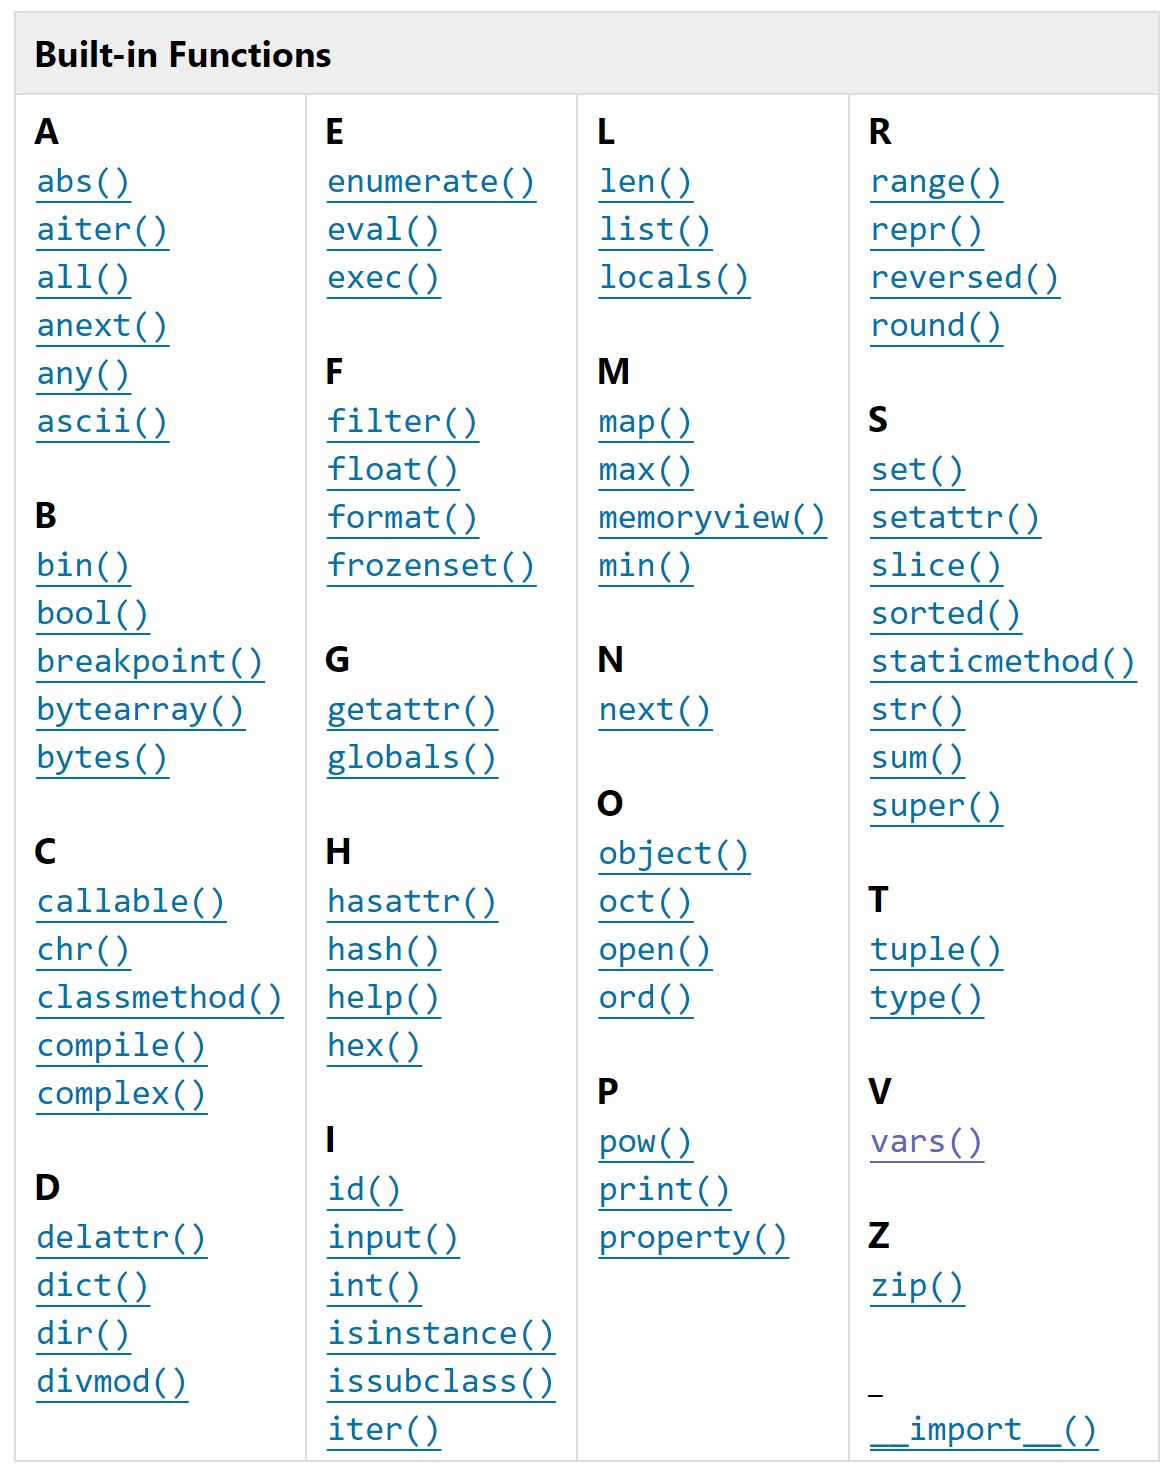
\includegraphics[width=0.6\textwidth]{images/built_in.JPG}
    \caption{Built-in Functions}
    \label{fig:misc-1}
\end{figure}

The \texttt{len()} function in Python is a built-in function that returns the length of an object. It's a versatile and commonly used tool that provides a convenient way to determine the number of elements in various data structures, such as strings, lists, tuples, dictionaries, and more.

\begin{codebox}
\begin{minted}{python}
# Example use of len() with a list
my_list = [1, 2, 3, 4, 5]
list_length = len(my_list)
print("Length of the list:", list_length)

# Example use of len() with a string
my_string = "Hello, World!"
print("Number of charactersin the string:", len(my_string))
\end{minted}
\end{codebox}

\newpage
\subsubsection{Map, Filter and Reduce}
The \texttt{map()}, \texttt{filter()}, and \texttt{reduce()} functions are powerful tools in functional programming, allowing for concise and efficient data transformations and computations over iterables. They help streamline code and make it more expressive by abstracting away common patterns of iteration and computation.
\begin{itemize}
    \item \textbf{\texttt{map()}}
    \begin{itemize}
        \item The \texttt{map()} function applies a specified function to each item in an iterable (such as a list) and returns a new iterator containing the results.
        \item Syntax: \texttt{map(function, iterable)}
        \item Example:
\begin{codebox}
\begin{minted}{python}
numbers = [1, 2, 3, 4, 5]
doubled = map(lambda x: x * 2, numbers)
print(list(doubled))  # Output: [2, 4, 6, 8, 10]
\end{minted}
\end{codebox}
        \item In this example, the \texttt{lambda x: x * 2} function is applied to each item in the \texttt{numbers} list, doubling each value.
    \end{itemize}
    
    \item \textbf{\texttt{filter()}}
    \begin{itemize}
        \item The \texttt{filter()} function constructs an iterator from elements of an iterable (such as a list) for which a specified function returns \texttt{True}.
        \item Syntax: \texttt{filter(function, iterable)}
        \item Example:
\begin{codebox}
\begin{minted}{python}
numbers = [1, 2, 3, 4, 5]
evens = filter(lambda x: x % 2 == 0, numbers)
print(list(evens))  # Output: [2, 4]
\end{minted}
\end{codebox}
        \item In this example, the \texttt{lambda x: x \% 2 == 0} function filters out only the even numbers from the \texttt{numbers} list.
    \end{itemize}
    
    \item \textbf{\texttt{reduce()}}
    \begin{itemize}
        \item The \texttt{reduce()} function is used to apply a rolling computation to sequential pairs of values in an iterable, producing a single accumulated result.
        \item Syntax: \texttt{reduce(function, iterable[, initializer])}
        \item Example:
\begin{codebox}
\begin{minted}{python}
from functools import reduce

numbers = [1, 2, 3, 4, 5]
total = reduce(lambda x, y: x + y, numbers)
print(total)  # Output: 15
\end{minted}
\end{codebox}
        \item In this example, the \texttt{lambda x, y: x + y} function is applied cumulatively to the items of the \texttt{numbers} list, resulting in the sum of all elements.
        \item In Python 3, the \texttt{reduce()} function is available in the \texttt{functools} module, so you do need to import it if you want to use \texttt{reduce()}. However, in Python 2, \texttt{reduce()} was a built-in function and didn't require an import.

    \end{itemize}
\end{itemize}

\newpage
\subsubsection{Iterator Functions}
Iterators are objects that implement the iterator protocol, which consists of two methods: \texttt{\_\_iter\_\_()} and \texttt{\_\_next\_\_()}. Iterators are used to iterate over a sequence of elements, such as lists, tuples, dictionaries, and custom objects.

\begin{itemize}
    \item \texttt{\_\_iter\_\_()}: This method returns the iterator object itself. It's called when you create an iterator using the \texttt{iter()} function or when an iterator is requested implicitly, such as in a \texttt{for} loop.
    
    \item \texttt{\_\_next\_\_()}: This method returns the next item from the iterator. It's called repeatedly to retrieve successive items from the iterator. When there are no more items to return, it raises a \texttt{StopIteration} exception.
\end{itemize}

\begin{codebox}
\begin{minted}{python}
class MyIterator:
    def __init__(self, limit):
        self.limit = limit
        self.current = 0

    def __iter__(self):
        return self

    def __next__(self):
        if self.current < self.limit:
            value = self.current
            self.current += 1
            return value
        else:
            raise StopIteration()
            

# Using the custom iterator
iterator = MyIterator(5)
for item in iterator:
    print(item)
\end{minted}
\end{codebox}

This example demonstrates how to create a simple custom iterator in Python that follows the iterator protocol. It generates values lazily, allowing for efficient memory usage, especially when dealing with large datasets or infinite sequences. The \texttt{\_\_iter\_\_()} method is called when an object is used in an iterable context, such as in a for loop, to obtain an iterator for the object. Iterators support the \texttt{next()} function, which is used to retrieve the next item from the iterator.\\

\newpage
Several Python built-in functions return iterators or objects that can be iterated over. Some of the most commonly used ones include:

\begin{itemize}
    \item \textbf{\texttt{iter()}}: This built-in function returns an iterator object for the given iterable. If the object is already an iterator, it returns itself. Otherwise, it calls the \texttt{\_\_iter\_\_()} method of the object to obtain an iterator.
    
    \item \textbf{\texttt{enumerate()}}: Returns an iterator that yields tuples containing a count (starting from zero by default) and the values obtained from iterating over the iterable.
    
    \item \textbf{\texttt{map()}}: Applies a given function to each item of an iterable (like a list or tuple) and returns an iterator that yields the results.
    
    \item \textbf{\texttt{filter()}}: Constructs an iterator from those elements of the iterable for which the function returns \texttt{True}.
    
    \item \textbf{File objects}: When reading from a file in Python, file objects return iterators over lines of the file. For example, when using a \texttt{for} loop to iterate over lines in a file, each iteration returns the next line from the file.
    
    \item \textbf{\texttt{range()}}: In Python 3, \texttt{range()} returns a range object that behaves like an iterator. It generates numbers within a specified range on demand rather than storing them all in memory.
\end{itemize}

The \texttt{iter()} function is used to obtain iterators from different types of iterables: a list, a custom callable, and a file object. Once you have an iterator, you can iterate over it using a \texttt{for} loop, use it with other functions that accept iterators, or manually call \texttt{next()} on it to retrieve the next element.

\begin{codebox}
\begin{minted}{python}
my_list = [1, 2, 3, 4, 5]
my_iterator = iter(my_list)
# Print the first element of the list
print(next(my_iterator))

# Iterate over the remaining elements using a for loop
for i in my_iterator:
    print(i)
\end{minted}
\end{codebox}

The \texttt{enumerate()} function is used to iterate over a sequence (such as a list, tuple, or string) while also tracking the index of each item. It returns an iterator that yields tuples containing both the index and the value of each item in the sequence.
\begin{codebox}
\begin{minted}{python}
my_list = ['apple', 'banana', 'cherry']

for index, value in enumerate(my_list):
    print(f"Index: {index}, Value: {value}")
\end{minted}
\end{codebox}

A range object is not technically an iterator, but it behaves similarly to one. The \texttt{range} object itself does \textbf{not} have a \texttt{next()} method.
\begin{codebox}
\begin{minted}{python}
# Create a range object with range(start, stop, step)
my_range = range(10, 0, -2)

# Print each number generated by the range object using next()
for i in my_range:
    print(i) # 10, 8, 6, 4, 2
\end{minted}
\end{codebox}

\newpage
\subsubsection{Generator Functions}
Generators are a \textit{special type of iterator} created using generator functions or generator expressions. Iterators are a general concept in Python for objects that can be iterated over, while generators are a specific implementation of iterators that provide a concise and efficient way to generate values lazily using generator functions or expressions. Generators are a powerful tool for working with iterators, especially when dealing with large datasets or when generating sequences dynamically.\\

Generator functions use the \texttt{yield} keyword to produce a series of values lazily, allowing for efficient memory usage and enabling the processing of large datasets or infinite sequences. Generators functions pause and resume their execution, allowing them to produce a sequence of values over time, rather than computing them all at once and storing them in memory.\\

When you use \texttt{yield} in a function, it turns that function into a generator. When the function is called, it doesn't execute immediately; instead, it returns a generator object. When you iterate over this generator object using a loop or other iteration constructs, the function starts executing, and when it encounters a \texttt{yield} statement, it temporarily suspends its execution and returns the value specified by yield. The next time you iterate over the generator, it resumes execution from where it left off.

\begin{codebox}
\begin{minted}{python}
def my_generator():
    yield 1
    yield 2
    yield 3

# Using the generator
gen = my_generator()
print(next(gen))  # Output: 1
print(next(gen))  # Output: 2
print(next(gen))  # Output: 3
# print(next(gen))  # Would raise StopIteration error
\end{minted}
\end{codebox}

\begin{codebox}
\begin{minted}{python}
def fibonacci():
    a, b = 0, 1
    while True:
        yield a
        a, b = b, a + b

# Create a Fibonacci generator
fib_gen = fibonacci()

# Print the first 10 Fibonacci numbers
print("First 10 Fibonacci numbers:")
for _ in range(10):
    print(next(fib_gen))
\end{minted}
\end{codebox}
The key here is that the tuple texttt{(b, a + b)} is created before any assignment occurs, so \texttt{a} is assigned the value of \texttt{b} and \texttt{b} is assigned the sum of the old values of \texttt{a} and \texttt{b}. This allows for a simultaneous update of both variables without needing a temporary variable.


\newpage
\subsubsection{Lambda Functions}
Lambda functions, also known as \textbf{anonymous functions}, are small, inline functions that are defined using the \texttt{lambda} keyword. Unlike regular functions defined using the \texttt{def} keyword, lambda functions are single-expression functions that can be created quickly without needing a formal \texttt{def} statement.

\begin{codebox}
\begin{minted}{python}
Adding two numbers
add = lambda x, y: x + y
print(add(3, 5))  # Output: 8

# Squaring a number
square = lambda x: x ** 2
print(square(4))  # Output: 16

# Checking if a number is even
is_even = lambda x: x % 2 == 0
print(is_even(5))  # Output: False
print(is_even(6))  # Output: True
\end{minted}
\end{codebox}

To create an iterator that yields only the even numbers from a given list, the \texttt{filter()} function is utilized along with a lambda function. The \texttt{filter()} function takes two arguments: the first argument is the lambda function that defines the condition for filtering, and the second argument is the iterable from which elements are filtered. In this case, the lambda function checks if a number \texttt{x} is even by performing the modulo operation \texttt{\% 2} and comparing the result to 0. The \texttt{filter()} function then returns an iterator that yields only those elements from the input iterable for which the lambda function returns \texttt{True}. Finally, the filtered iterator is iterated over to print the even numbers.

\begin{codebox}
\begin{minted}{python}
# Define a list of numbers
numbers = [1, 2, 3, 4, 5, 6, 7, 8, 9, 10]

# Use filter() with a lambda function
even_numbers_iterator = filter(lambda x: x % 2 == 0, numbers)

# Iterate over the filtered iterator and print the even numbers
print("Even numbers:")
for num in even_numbers_iterator:
    print(num)
\end{minted}
\end{codebox}

%\begin{codebox}
%\begin{minted}{python}
%
%\end{minted}
%\end{codebox}





\section{Object-Oriented Programming (OOP)}

\subsection{Terms and Programming Concepts}

\begin{itemize}
    \item \textbf{Class:} A class is a blueprint for creating objects. It defines the attributes (variables) and methods (functions) that all instances of the class will have.
    
    \item \textbf{Instance:} An instance is a specific realization of a class. It is an individual object created from a class, with its own set of attributes and methods.
    
    \item \textbf{Attribute:} An attribute is a piece of data associated with a particular object. It can be thought of as a variable that belongs to an object.
    
    \item \textbf{Method:} A method is a function defined within a class. It operates on the data within the class and can modify the state of the object or perform some action.
    
    \item \textbf{Object:} In Python, everything is an object. An object is a collection of data (variables) and methods (functions) that act on the data.
    
    \item \textbf{Type:} The type of an object determines what class it belongs to. It defines the attributes and methods that the object will have.
\end{itemize}

\begin{codebox}
\begin{minted}{python}
# Define a Dog class
class Dog:
    # Constructor method to initialize object attributes
    def __init__(self, name, breed, age):
        self.name = name  
        self.breed = breed
        self.age = age

    # Method to get description of the dog
    def get_description(self):
        return f"{self.name} is a {self.age}-year-old {self.breed}."


# Create an instance of the Dog class
my_dog = Dog('Buddy', 'Golden Retriever', 3)

# Accessing age attribute directly
print(my_dog.age)  # Output: 3

# Call the get_description method to print dog's description
print(my_dog.get_description())

# Print the type of the object and the name of the class
print(type(my_dog))           # Output: <class '__main__.Dog'>
print(type(my_dog).__name__)  # Output: Dog
\end{minted}
\end{codebox}

\subsubsection{The \texttt{\_\_init\_\_()} method}

The \texttt{\_\_init\_\_} method is a special method used for initializing objects of a class. It is also known as a constructor method. The \texttt{\_\_init\_\_} method is called automatically whenever a new instance of the class is created.

\newpage
\subsubsection{Instance and Class Variables}

\begin{itemize}
\item \textbf{Instance Variables}\\
Variables that are unique to each instance of a class. They are defined within the constructor method (\texttt{\_\_init\_\_}) using the self keyword. Each instance of the class has its own copy of instance variables. Instance variables hold data that is specific to each object or instance of the class.

\item  \textbf{Class Variables}\\
Variables that are shared among all instances of a class. They are defined outside of any method, typically at the beginning of the class definition. Class variables are accessed using the class name itself, rather than through instances of the class. They are used to store data that is common to all instances of the class.
\end{itemize}

\begin{codebox}
\begin{minted}{python}
class Car:
    # Class variables
    wheels = 4
    total_cars = 0  # Counter for total number of cars

    def __init__(self, make, model):
        # Instance variables
        self.make = make
        self.model = model
        # Increment the total number of cars when a new instance is created
        Car.total_cars += 1


# Creating instances
car1 = Car('Toyota', 'Camry')
car2 = Car('Honda', 'Accord')
car3 = Car('Ford', 'Focus')

# Accessing class variable total_cars
print("Total number of cars:", Car.total_cars)  # Output: 3

# Accessing class variable using instance name (not recommended)
print(car1.total_cars) # Output: 3
\end{minted}
\end{codebox}

Although accessing class variables using an instance name works in Python, it's clearer and more conventional to access them using the class name directly. This helps to distinguish between instance variables and class variables clearly.

\newpage
\subsubsection{The \texttt{\_\_dict\_\_} Attribute}
The \texttt{\_\_dict\_\_} is a special attribute that is present in every object and holds the object's attributes. It is a dictionary that maps attribute names (as keys) to their corresponding values. You can use \texttt{\_\_dict\_\_} to access, manipulate, or inspect the attributes of an object dynamically.

\begin{codebox}
\begin{minted}{python}
class MyClass:
    class_variable = 0

    def __init__(self, x, y):
        self.x = x  
        self.y = y  


obj1 = MyClass(10, 20)

# Printing instance variables of obj1
print(obj1.__dict__)  # Output: {'x': 10, 'y': 20}

# Printing class variables and methods of MyClass
print(MyClass.__dict__)  # {'__module__': '__main__', 'class_variable': 0, ...
\end{minted}
\end{codebox}

\subsubsection{The \texttt{vars()} Function}

The \texttt{vars()} function is closely related to the \texttt{\_\_dict\_\_} attribute. It returns the \texttt{\_\_dict\_\_} attribute of an object if it exists, allowing you to access the object's attributes in the form of a dictionary. This function provides a convenient way to inspect the attributes of an object dynamically, similar to directly accessing the \texttt{\_\_dict\_\_} attribute.

\begin{codebox}
\begin{minted}{python}
class MyClass:
    class_variable = 0

    def __init__(self, x, y):
        self.x = x  
        self.y = y  


obj1 = MyClass(10, 20)

# Printing instance variables of obj1
print(vars(obj1))

# Printing class variables and methods of MyClass
print(vars(MyClass))
\end{minted}
\end{codebox}

\begin{minted}[
    bgcolor=white,
    frame=leftline,
    framesep=2mm,
    rulecolor=black,
    linenos=false, 
]{text}
{'x': 10, 'y': 20}
{
    '__module__': '__main__', 
    'class_variable': 0, 
    '__init__': <function MyClass.__init__ at 0x00000239ACED7600>, 
    '__dict__': <attribute '__dict__' of 'MyClass' objects>, ...
}
\end{minted}

%%%%%%%%%%%%%%%%%%%%%%%%%%%%%%%%%%%%%%%%%%%%%%%%%%%%%%%%%%%%%%%%%%%%%%%%%%
\newpage
\subsection{Core Syntax Operations}

\subsubsection{Magic Methods}
Magic methods, also known as dunder methods (short for "double underscore"), are special methods that have double underscore prefixes and suffixes, like \texttt{\_\_add\_\_}. These methods enable customization of how objects behave in certain contexts, such as arithmetic operations, comparison operations, and object creation.\\

\textbf{Comparison methods}\\[0.1cm]
\begin{tabular}{|p{3cm}|p{4cm}|p{8cm}|}
\hline
\textbf{Operator} & \textbf{Magic method} & \textbf{Implementation meaning or purpose} \\
\hline
\texttt{==} & \texttt{\_\_eq\_\_(self, other)} & Equality operator \\
\texttt{!=} & \texttt{\_\_ne\_\_(self, other)} & Inequality operator \\
\texttt{<} & \texttt{\_\_lt\_\_(self, other)} & Less-than operator \\
\texttt{>} & \texttt{\_\_gt\_\_(self, other)} & Greater-than operator \\
\texttt{<=} & \texttt{\_\_le\_\_(self, other)} & Less-than-or-equal-to operator \\
\texttt{>=} & \texttt{\_\_ge\_\_(self, other} & Greater-than-or-equal-to operator \\
\hline
\end{tabular}

\vspace{0.5cm}

\textbf{Unary operators and functions}\\[0.1cm]
\begin{tabular}{|p{3cm}|p{4cm}|p{8cm}|}
\hline
\textbf{Operator} & \textbf{Magic method} & \textbf{Implementation meaning or purpose} \\
\hline
\texttt{+} & \texttt{\_\_pos\_\_(self)} & Unary positive, like \texttt{a = +b} \\
\texttt{-} & \texttt{\_\_neg\_\_(self)} & Unary negative, like $a = -b$ \\
\texttt{abs()} & \texttt{\_\_abs\_\_(self)} & Behavior for \texttt{abs()} function \\
\texttt{round(a, b)} & \texttt{\_\_round\_\_(self, b)} & Behavior for \texttt{round()} function \\
\hline
\end{tabular}

\vspace{0.5cm}

\textbf{Common, binary operators and functions}\\[0.1cm]
\begin{tabular}{|p{2cm}|p{5cm}|p{8cm}|}
\hline
\textbf{Operator} & \textbf{Magic method} & \textbf{Implementation meaning or purpose} \\
\hline
\texttt{+} & \texttt{\_\_add\_\_(self, other)} & Addition operator \\
\texttt{-} & \texttt{\_\_sub\_\_(self, other)} & Subtraction operator \\
\texttt{*} & \texttt{\_\_mul\_\_(self, other)} & Multiplication operator \\
\texttt{//} & \texttt{\_\_floordiv\_\_(self, other)} & Integer division operator \\
\texttt{/} & \texttt{\_\_truediv\_\_(self, other)} & Division operator \\
\texttt{\%} & \texttt{\_\_mod\_\_(self, other)} & Modulo operator \\
\texttt{**} & \texttt{\_\_pow\_\_(self, other)} & Exponential (power) operator \\
\hline
\end{tabular}

\vspace{0.5cm}

\textbf{Augmented operators and functions}\\[0.1cm]
\begin{tabular}{|p{2cm}|p{5cm}|p{8cm}|}
\hline
\textbf{Operator} & \textbf{Magic method} & \textbf{Implementation meaning or purpose} \\
\hline
\texttt{+=} & \texttt{\_\_iadd\_\_(self, other)} & Addition and assignment operator \\
\texttt{-=} & \texttt{\_\_isub\_\_(self, other)} & Subtraction and assignment operator \\
\texttt{*=} & \texttt{\_\_imul\_\_(self, other)} & Multiplication and assignment operator \\
\texttt{//=} & \texttt{\_\_ifloordiv\_\_(self, other)} & Integer division and assignment operator \\
\texttt{/=} & \texttt{\_\_idiv\_\_(self, other)} & Division and assignment operator \\
\texttt{\%=} & \texttt{\_\_imod\_\_(self, other)} & Modulo and assignment operator \\
\texttt{**=} & \texttt{\_\_ipow\_\_(self, other)} & Exponential (power) and assignment operator \\
\hline
\end{tabular}
\vspace{0.5cm}

\newpage
\textbf{Type conversion methods}\\[0.1cm]
\begin{tabular}{|p{2cm}|p{4cm}|p{9cm}|}
\hline
\textbf{Function} & \textbf{Magic method} & \textbf{Implementation meaning or purpose} \\
\hline
\texttt{int()} & \texttt{\_\_int\_\_(self)} & Conversion to integer type \\
\texttt{float()} & \texttt{\_\_float\_\_(self)} & Conversion to float type \\
\texttt{oct()} & \texttt{\_\_oct\_\_(self)} & Conversion to string, containing an octal representation \\
\texttt{hex()} & \texttt{\_\_hex\_\_(self)} & Conversion to string, containing a hex representation \\
\hline
\end{tabular}

\vspace{0.5cm}

\textbf{Object introspection}\\[0.1cm]
\begin{tabular}{|p{2cm}|p{5.5cm}|p{7.5cm}|}
\hline
\textbf{Function} & \textbf{Magic method} & \textbf{Implementation meaning or purpose} \\
\hline
\texttt{str()} & \texttt{\_\_str\_\_(self)} & Handling str() function calls \\
repr() & \texttt{\_\_repr\_\_(self)} & Handling repr() function calls \\
\texttt{format()} & \texttt{\_\_format\_\_(self, formatstr)} & When string formatting is applied to an object \\
\texttt{hash()} & \texttt{\_\_hash\_\_(self)} & Handling hash() function calls \\
\texttt{dir()} & \texttt{\_\_dir\_\_(self)} & Handling dir() function calls \\
\texttt{bool()} & \texttt{\_\_nonzero\_\_(self)} & Handling bool() calls (\texttt{\_\_bool\_\_()} in Python 3)
 \\
\hline
\end{tabular}

\vspace{0.5cm}

\textbf{Object retrospection}\\[0.1cm]
\begin{tabular}{|p{4.5cm}|p{6cm}|p{4.5cm}|}
\hline
\textbf{Function} & \textbf{Magic method} & \textbf{Implementation} \\
\hline
\texttt{isinstance(obj, class)} & \texttt{\_\_instancecheck\_\_(self, obj)} & Handling isinstance() calls \\
\texttt{issubclass(subclass, class)} & \texttt{\_\_subclasscheck\_\_(self, subclass)} & Handling issubclass() calls \\
\hline
\end{tabular}

\vspace{0.5cm}

\textbf{Object attribute access}\\[0.1cm]
\begin{tabular}{|p{3.5cm}|p{6cm}|p{5.5cm}|}
\hline
\textbf{Expression} & \textbf{Magic method} & \textbf{Implementation} \\
\hline
\texttt{obj.attr} & \texttt{\_\_getattr\_\_(self, attr)} & Access to a non-existing attribute \\
\texttt{obj.attr} & \texttt{\_\_getattribute\_\_(self, attr)} & Access to an existing attribute \\
\texttt{obj.attr = val} & \texttt{\_\_setattr\_\_(self, attr, val)} & Setting an attribute value \\
\texttt{del object.attr} & \texttt{\_\_delattr\_\_(self, attr)} & Deleting an attribute \\
\hline
\end{tabular}

\vspace{0.5cm}

\textbf{Methods allowing access to containers}\\[0.1cm]
\begin{tabular}{|p{4.5cm}|p{6cm}|p{4.5cm}|}
\hline
\textbf{Expression} & \textbf{Magic method} & \textbf{Implementation} \\
\hline
\texttt{len(container)} & \texttt{\_\_len\_\_(self)} & Returns number of elements of the container \\
container[key] & \texttt{\_\_getitem\_\_(self, key)} & Fetching an element identified by the key\\
\texttt{container[key] = value} & \texttt{\_\_setitem\_\_(self, key, value)} & Setting a value to an element identified by the key\\
\texttt{del container[key]} & \texttt{\_\_delitem\_\_(self, key)} & Deleting an element identified by the key\\
\texttt{for el in container} & \texttt{\_\_iter\_\_(self)} & Returns an iterator for the container \\
\texttt{item in container} & \texttt{\_\_contains\_\_(self, item)} & Returns true if container has the item \\
\hline
\end{tabular}

\vspace{0.5cm}





By implementing these methods in a class, you can customize how instances of the class behave in various contexts, making your code more expressive and idiomatic.

\newpage
\subsubsection{Comparison Methods}

This code demonstrates the use of the \texttt{\_\_eq\_\_} method in classes, along with the behavior of the equality operator (\texttt{==}).

\begin{codebox}
\begin{minted}{python}
class Point():
    def __init__(self, x, y):
        self.x = x
        self.y = y
        
    def __eq__(self, other):
        return (self.x, self.y) == (other.x, other.y)

point1=Point(1,2)
point2=Point(1,2)

print(point1.__eq__(point2))  # Output: True
print(point1 == point2)  # Output: True
\end{minted}
\end{codebox}

\subsubsection{Accessing Containers}

The \texttt{\_\_getitem\_\_} method is a special method that allows objects to support indexing and slicing operations. It is called when you use square brackets (\texttt{[]}) to access elements from a container object, such as lists, dictionaries, or custom classes.

\begin{codebox}
\begin{minted}{python}
class MyContainer:
    def __init__(self, data):
        self.data = data

    def __getitem__(self, index):
        return self.data[index]

container = MyContainer([1, 2, 3, 4, 5])
print(container[2])  # Output: 3
\end{minted}
\end{codebox}

\subsubsection{Numeric Methods}
The \texttt{\_\_abs\_\_()} method is a special method that allows objects to define custom behavior for the built-in \texttt{abs()} function when applied to instances of the class.

\begin{codebox}
\begin{minted}{python}
class MyNumber:
    def __init__(self, value):
        self.value = value
    
    def __abs__(self):
        return abs(self.value)

x = MyNumber(-5)
print(abs(x))  # Output: 5
\end{minted}
\end{codebox}

\newpage
\subsubsection{Customizing Object Behavior}

The methods \texttt{\_\_call\_\_}, \texttt{\_\_repr\_\_}, and \texttt{\_\_str\_\_} are special methods that allow to customize the behavior of objects.

\begin{itemize}
    \item \textbf{The \_\_call\_\_ method:} allows the instance of \texttt{MyClass} to behave like a function. It is called when an instance of the class is used as if it were a function, for example, \texttt{obj()}.
    \item \textbf{The \_\_repr\_\_ method:} provides an unambiguous representation of the object, primarily meant for developers. It should ideally be valid Python code to recreate the object. It is used for debugging, logging, or creating new instances of the object.
    \item \textbf{The \_\_str\_\_ method:} provides a more user-friendly string representation of the object. It is called when the built-in function \texttt{str()} is used on the object, or when the object is passed to the \texttt{print()} function.
\end{itemize}

\begin{codebox}
\begin{minted}{python}
class MyClass:
    def __init__(self, x):
        self.x = x

    def __call__(self, y):
        # Allows instances of a class to be invoked like functions
        return self.x + y

    def __repr__(self):
        # Returns a string representation for developers
        return f'MyClass({self.x})'

    def __str__(self):
        # Returns a user-friendly string representation of the object
        return f'MyClass object with x = {self.x}'

# Creating an instance of MyClass
obj = MyClass(5)

# Using __call__ method
print(obj(3))

# Using __repr__ method
print(repr(obj))
print([obj]) # Calls __repr__ for each object in the list
logging.error(repr(obj)) # Using repr() for debugging/logging
#print(`obj`)  # Equivalent to repr(obj), in Python 2.x

# Using __str__ method, calls obj.__repr__() if __str__ is not defined
print(obj) 
print(str(obj))
print(f'{obj}')
print("%s" % obj)
print("{}".format(obj))
print(MyClass(2))
\end{minted}
\end{codebox}

\newpage
\subsubsection{Object Attribute Access}
The \_\_getattr\_\_, \_\_setattr\_\_, and \_\_delattr\_\_ methods are special methods that allow you to customize attribute access, assignment, and deletion behavior in objects.

\begin{itemize}
    \item \textbf{\texttt{\_\_getattr\_\_}}: This method is called when an attribute lookup fails. It allows you to define custom behavior for accessing attributes that don't exist in an object's namespace.
    
    \item \textbf{\texttt{\_\_setattr\_\_}}: This method is called when an attribute assignment is made. It allows you to customize behavior when setting attributes.
    
    \item \textbf{\texttt{\_\_delattr\_\_}}: This method is called when an attribute deletion is requested. It allows you to customize behavior when deleting attributes.
\end{itemize}

\begin{codebox}
\begin{minted}{python}
class DynamicAttributes:
    def __init__(self):
        self.data = {}

    def __getattr__(self, name):
        if name in self.data:
            return self.data[name]
        else:
            raise AttributeError(f"Object has no attribute '{name}'")

    def __setattr__(self, name, value):
        print(f"Setting attribute '{name}' to '{value}'")
        self.data[name] = value

    def __delattr__(self, name):
        if name in self.data:
            del self.data[name]
            print(f"Deleted attribute '{name}'")
        else:
            raise AttributeError(f"Object has no attribute '{name}'")


# Creating an instance of DynamicAttributes
obj = DynamicAttributes()

# Setting attribute
obj.x = 10  # Output: Setting attribute 'x' to '10'

# Accessing attribute
print(obj.x)  # Output: 10

# Deleting attribute
del obj.x  # Output: Deleted attribute 'x'

# Trying to access deleted attribute
print(obj.x)  # Raises AttributeError
\end{minted}
\end{codebox}

% TODO
%\subsubsection{Object intro- and retrospection}

%\subsubsection{Extending class implementations to support additional core syntax operations}

%%%%%%%%%%%%%%%%%%%%%%%%%%%%%%%%%%%%%%%%%%%%%%%%%%%%%%%%%%%%%%%%%%%%%%%%%%
\newpage
\subsection{Inheritance, Polymorphism, and Composition}

\subsubsection{Superclasses and Subclasses}
\begin{itemize}
    \item \textbf{Superclasses:}
    Provide a blueprint or template for the subclasses to follow.
    \item \textbf{Subclasses:}
    Inherit properties (attributes) and behaviors (methods) from their superclasses.
\end{itemize}

\begin{codebox}
\begin{minted}{python}
class Animal:
    def speak(self):
        print("This animal makes a sound.")

class Dog(Animal):
    def speak(self):
        print("Woof!")

class Cat(Animal):
    def speak(self):
        print("Meow!")


# Create instances of Dog and Cat
dog = Dog()
cat = Cat()
\end{minted}
\end{codebox}
The code defines three classes: \texttt{Animal}, \texttt{Dog}, and \texttt{Cat}. The \texttt{Animal} class has a method named \texttt{speak} that prints "This animal makes a sound." Both the \texttt{Dog} and \texttt{Cat} classes are subclasses of \texttt{Animal}, inheriting the \texttt{speak} method. The \texttt{Dog} class overrides the \texttt{speak} method with its own implementation to print "Woof!", and similarly, the \texttt{Cat} class overrides the \texttt{speak} method with its own implementation to print "Meow!".

\subsubsection{Reflection: \texttt{isinstance()} and \texttt{issubclass()}}

Reflection refers to the ability of a program to examine and modify its own structure, behavior, and metadata at runtime. This includes the capability to inspect classes, functions, modules, and objects to retrieve information about their attributes, methods, and other properties

\begin{itemize}
    \item \textbf{Introspection}: Examining the type and structure of objects at runtime.
    \item \textbf{Dynamic instantiation}: Creating instances of classes dynamically, based on runtime information.
    \item \textbf{Attribute and method manipulation}: Accessing and modifying attributes and methods of objects dynamically.
    \item \textbf{Dynamic module loading}: Loading modules dynamically during program execution.
    \item \textbf{Metaprogramming}: Writing code that generates or modifies other code.
\end{itemize}

\newpage
The \texttt{isinstance()} and \texttt{issubclass()} function are two built-in functions in Python used for type checking and inheritance checking respectively.

\begin{itemize}
\item \textbf{\texttt{isinstance()}:} This function is used to check if an object belongs to a particular class or any subclass of that class. It takes two arguments: the object and the class (or a tuple of classes). It returns True if the object is an instance of the specified class or any of its subclasses, otherwise, it returns False.
\begin{codebox}
\begin{minted}{python}
print(isinstance(dog, Animal))  # Output: True
print(isinstance(dog, Dog))     # Output: True
print(isinstance(cat, Dog))     # Output: False
\end{minted}
\end{codebox}

\item \textbf{\texttt{issubclass()}:} This function is used to check if a class is a subclass of another class. It takes two arguments: the subclass and the superclass. It returns True if the first class is indeed a subclass of the second class, otherwise, it returns False. Reflection enables dynamic manipulation of code and data structures, allowing for tasks such as:

\begin{codebox}
\begin{minted}{python}
print(issubclass(Dog, Animal))  # Output: True
print(issubclass(Cat, Animal))  # Output: True
print(issubclass(Cat, Cat))     # Output: True
\end{minted}
\end{codebox}

Cat is a subclass of Animal, and \texttt{issubclass(Cat, Cat)} correctly outputs \texttt{True} because a class is considered a subclass of itself. This behavior is expected in Python.
\end{itemize}

\subsubsection{Introspection}
Introspection refers to the ability of a program to examine the type, properties, and methods of objects at runtime. It allows you to dynamically inspect and manipulate objects, classes, functions, and modules within your code. Python's introspection capabilities are facilitated by various built-in functions and modules that provide information about objects. Some of the commonly used functions and modules for introspection include:

\begin{itemize}
    \item \textbf{type():} Returns the type of an object.
    \item \textbf{dir():} Returns a list of attributes and methods of an object.
    \item \textbf{getattr():} Retrieves the value of an attribute of an object dynamically, based on its name.
    \item \textbf{hasattr():} Checks whether an object has a specific attribute.
    \item \textbf{callable():} Checks whether an object is callable (i.e., whether it can be called as a function).
    \item \textbf{help():} Provides interactive help on objects, modules, functions, classes, and methods.
\end{itemize}

\begin{codebox}
\begin{minted}{python}
class Cat:
    def __init__(self, name, color):
        self.name = name
        self.color = color

my_cat = Cat("Whiskers", "gray")

# Example using getattr and hasattr
print(getattr(my_cat, "name"))  # Output: Whiskers
print(hasattr(my_cat, "name"))   # Output: True
print(hasattr(my_cat, "age"))    # Output: False
\end{minted}
\end{codebox}


\newpage
\subsubsection{Inheritance vs. Composition}
In object-oriented programming, inheritance and composition are two fundamental concepts used for structuring and organizing code.\\

\begin{itemize}
\item \textbf{Inheritance}: A new class (subclass or derived class) is created by inheriting properties and behaviors from an existing class (superclass or base class). It promotes code reusability by allowing subclasses to inherit attributes and methods from a superclass. Subclasses can then add their own attributes and methods or override the ones inherited from the superclass.

\begin{codebox}
\begin{minted}{python}
class Vehicle:
    def drive(self):
        return "Vehicle is being driven"

class Car(Vehicle):
    def drive(self):
        return "Car is being driven"
\end{minted}
\end{codebox}


\item \textbf{Composition}: A class contains objects of other classes as members. Instead of inheriting their behavior, the containing class delegates tasks to contained objects. It allows for building complex objects by combining simpler ones. Each object maintains its own behavior, and the containing object orchestrates their interactions.

\begin{codebox}
\begin{minted}{python}
class Engine:
    def start(self):
        return "Engine started"

class Car:
    def __init__(self):
        self.engine = Engine()
        
    def start(self):
        return self.engine.start()
\end{minted}
\end{codebox}
\end{itemize}

\subsubsection{Real-life problems using "is a" and "has a" relations}

\begin{itemize}
\item \textbf{Inheritance: "is-a" Relationship}\\
Subclasses are specialized versions of their superclass. Subclasses inherit common properties and behaviors from their superclass. For example, a Car is a type of Vehicle.\\

\item \textbf{Composition: "has-a" Relationship}\\
Classes contain instances of other classes as components. This allows them to utilize the functionalities of those components. For example, a Car has an Engine, Wheel, and Transmission.
\end{itemize}

\newpage
\subsubsection{Class Hierarchies}
Class hierarchies are structures that organize classes into a tree-like hierarchy, where classes can inherit attributes and methods from their parent classes. This enables code reuse, modularity, and the implementation of polymorphism.

\subsubsection{Single vs. Multiple Inheritance}
Inheritance allows a class to inherit attributes and methods from another class. There are two types of inheritance: single inheritance and multiple inheritance.\\

\begin{itemize}
\item \textbf{Single Inheritance:}
Class inherits from only one base class.\\

\begin{codebox}
\begin{minted}{python}
class Animal:
    def sleep(self):
        return "Animal sleeps"

class Dog(Animal):
    def bark(self):
        return "Dog barks"


dog = Dog()

# Dog inherits from Animal
# Dog class has access to the methods of Animal class
print(dog.sleep())  # Output: "Animal sleeps"
print(dog.bark())   # Output: "Dog barks"
\end{minted}
\end{codebox}

\item \textbf{Multiple Inheritance:}
Class inherits from multiple base classes.\\


\begin{codebox}
\begin{minted}{python}
class Animal:
    def sleep(self):
        return "Animal sleeps"

class Pet:
    def play(self):
        return "Pet plays"

class Dog(Animal, Pet):
    def bark(self):
        return "Dog barks"


dog = Dog()

# Dog inherits from both Animal and Pet
# Dog class has access to the methods of Animal and Pet classes
print(dog.sleep())  # Output: "Animal sleeps"
print(dog.play())   # Output: "Pet plays"
print(dog.bark())   # Output: "Dog barks"
\end{minted}
\end{codebox}
\end{itemize}

\newpage
\subsubsection{Polymorphism}
Polymorphism refers to the ability of different objects to respond to the same method or function call in different ways. It allows objects of different classes to be treated as objects of a common superclass, enabling code reuse and flexibility in design. There are two main types of polymorphism:

\begin{itemize}
    \item \textbf{Method Overriding:} This occurs when a subclass provides a specific implementation of a method that is already defined in its superclass. The method in the subclass overrides the method with the same name and signature in the superclass.
    
    \item \textbf{Operator Overloading:} This allows operators to have different implementations depending on the types of operands involved. Python provides special methods, often referred to as "magic methods" or "dunder methods", to enable operator overloading.
\end{itemize}

\subsubsection{Duck Typing}
Duck typing is a concept, where the type or class of an object is determined not by its inheritance hierarchy or explicit declaration, but by its behavior. In other words, an object's suitability is determined by whether it behaves like a duck, if it walks like a duck and quacks like a duck, then it must be a duck.
This means that if an object supports the necessary methods or attributes required by a particular operation, it can be used in that context regardless of its actual class or inheritance.

\begin{codebox}
\begin{minted}{Python}
class Duck:
    def quack(self):
        print("Quack!")

class Robot:
    def quack(self):
        print("I'm quacking like a duck!")

def make_it_quack(obj):
    obj.quack()

# Instances of Duck and Robot
duck = Duck()
robot = Robot()

# Duck typing allows any object with a quack() method
make_it_quack(duck)   # Output: "Quack!"
make_it_quack(robot)  # Output: "I'm quacking like a duck!"
\end{minted}
\end{codebox}

\begin{figure}[h!]
    \centering
    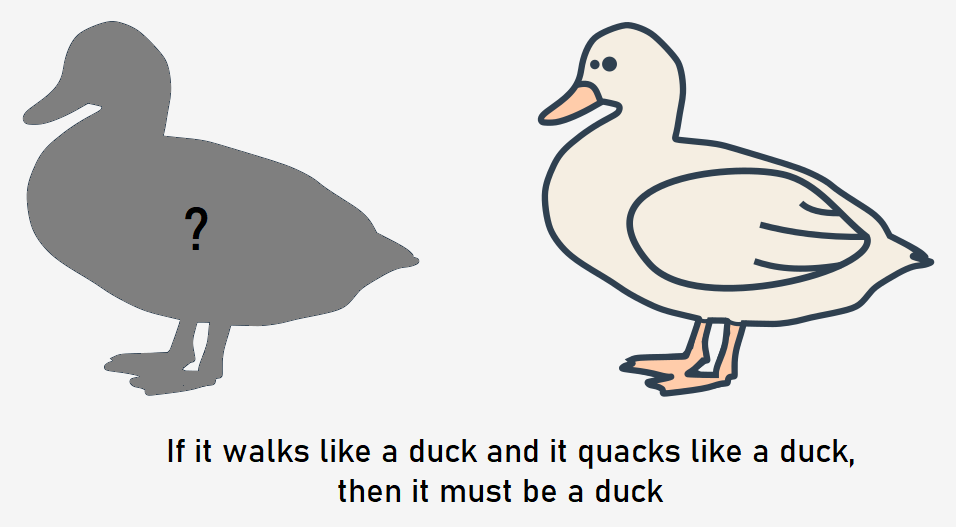
\includegraphics[width=0.4\textwidth]{images/twoDucks.png}
    \caption{Duck typing}
    \label{fig:example-1}
\end{figure}

%\begin{quote}
%\textit{``If it looks like a duck, swims like a duck, and quacks like a duck, \\ then it probably is a duck.''}
%\end{quote}


\newpage
\subsubsection{Diamond Problem: Method Resolution Order (MRO)}
The Diamond problem does not exist in Python because it gives preference to the class that is inherited first. The Method Resolution Order (MRO) defines the order in which Python looks for methods and attributes in a class hierarchy. When a method is called on an object, Python searches for it starting from the class of the object and then follows the MRO to find the method in the inheritance hierarchy.

\begin{codebox}
\begin{minted}{python}
class A:
    def hello(self):
        print('Hello from class A')
 
class B(A):
    def hello(self):
        print('Hello from class B')
 
class C(A):
    def hello(self):
        print('Hello from class C')
 
class D(B, C):
    pass

D().hello()  # Output: Hello from class B
\end{minted}
\end{codebox}

\texttt{D().hello()} calls the \texttt{hello()} method of class D. Since class D doesn't have its own \texttt{hello()} method, Python looks for it in the classes D inherits from, following the MRO. Therefore, the output of \texttt{D().hello()} is "Hello from class B".

\begin{codebox}
\begin{minted}{python}
# Output the MRO for class D
print(D.__mro__)
\end{minted}
\end{codebox}
\begin{minted}[
    bgcolor=white,
    frame=leftline,
    framesep=2mm,
    rulecolor=black,
    linenos=false,
]{text}
(__main__.D, __main__.B, __main__.C, __main__.A, object)
\end{minted}

Python will look for the \texttt{hello} method in class D first, then in class B, then in class C, then in class A, and finally in the base class \texttt{object}. Given the provided class hierarchy, the MRO for class D is as follows: 
$D \to B \to C \to A \to \texttt{object}$\\

\newpage
\subsubsection{The Inheritance Tangle}
The diamond inheritance problem is a common challenge encountered in object-oriented programming, particularly in languages like Python that support multiple inheritance. This issue arises when a class inherits from two or more classes, each of which in turn inherits from a common base class. As a result, the inheritance hierarchy forms a diamond shape, with multiple paths leading to the same base class.

\begin{codebox}
\begin{minted}{python}
class A:
    def info(self):
        print('Class A')

class B(A):
    def info(self):
        print('Class B')

class MyClass(A, B):
    pass

MyClass().info()
\end{minted}
\end{codebox}

\begin{minted}[
    bgcolor=white,
    frame=leftline,
    framesep=2mm,
    rulecolor=black,
    linenos=false, 
]{text}
---------------------------------------------------------------------------
TypeError                                 Traceback (most recent call last)
Cell In[24], line 9
      6     def info(self):
      7         print('Class B')
----> 9 class MyClass(A, B):
     10     pass
     12 MyClass().info()

TypeError: Cannot create a consistent method resolution
order (MRO) for bases A, B
\end{minted}

The error encountered stems from the diamond inheritance problem in Python. When a class like \texttt{MyClass(A, B)} is defined, inheriting from both \texttt{A} and \texttt{B}, Python faces difficulty in establishing a consistent method resolution order (MRO) due to conflicting inheritance paths. In this scenario, both \texttt{A} and \texttt{B} serve as base classes for \texttt{MyClass}, sharing a common ancestor (\texttt{object} by default in Python 3). However, Python's MRO algorithm struggles to determine a linear order for method search amidst these conflicting paths.\\

To resolve this error, it's necessary to redesign the class hierarchy to avoid the diamond inheritance problem. A common approach involves ensuring that each class inherits from its base classes via a single, unambiguous path.


\newpage
\subsubsection{The \texttt{super()} Function}
\texttt{super()} is a built-in function that allows you to call methods and access attributes from the parent class within a subclass. It provides a way to invoke methods defined in the superclass (parent class) of an object, enabling better code reuse and maintaining a clean inheritance structure.\\

The \texttt{super()} function is typically used inside methods of a subclass to call the corresponding method of the superclass. This is particularly useful when the subclass overrides a method defined in the superclass but still wants to execute the overridden method's behavior. By using \texttt{super()}, you can avoid explicitly naming the parent class and make your code more flexible to changes in the inheritance hierarchy.

\begin{codebox}
\begin{minted}{python}
class Parent:
  def __init__(self, msg):
    print("Calling Parent class constructor")
    self.message = msg

  def printmessage(self):
    print(self.message)

class Child(Parent):
  def __init__(self, msg):
    print("Calling Child class constructor")
    super().__init__(msg)


obj = Child("Hello, and welcome!")
obj.printmessage()
\end{minted}
\end{codebox}

\begin{minted}[
    bgcolor=white,
    frame=leftline,
    framesep=2mm,
    rulecolor=black,
    linenos=false,
]{text}
Calling Child class constructor
Calling Parent class constructor
Hello, and welcome!
\end{minted}

%%%%%%%%%%%%%%%%%%%%%%%%%%%%%%%%%%%%%%%%%%%%%%%%%%%%%%%%%%%%%%%%%%%%%%%%%%
% 1.8
\newpage
\subsubsection{Subclassing Built-in Classes}
%\subsubsection{Inheriting properties from built-in classes}
Inheriting properties from built-in classes allows for flexible customization of classes to suit specific needs without having to start from scratch. This is often done to customize behavior, add functionality, or override existing methods. However, it's essential to be cautious when subclassing built-ins, as it may lead to unexpected behavior if not done carefully.

\begin{codebox}
\begin{minted}{python}
class CustomList(list):
    def __init__(self, *args):
        super().__init__(*args)

    def append_twice(self, item):
        self.append(item)
        self.append(item)
    
    def sum(self):
        return sum(self)
    
    def average(self):
        if len(self) == 0:
            return 0
        return sum(self) / len(self)


# Creating an instance of CustomList
my_list = CustomList([1, 2, 3, 4, 5])

# Inheriting built-in method 'append'
my_list.append(6)

# Adding custom method 'append_twice'
my_list.append_twice(7)

print("Modified List:", my_list) # [1, 2, 3, 4, 5, 6, 7, 7]
print(my_list.sum()) # 35
print(my_list.average()) # 4.375
\end{minted}
\end{codebox}

Inheritance allows to acquire properties and methods from built-in classes such as \texttt{list}, \texttt{dict}, or \texttt{str}. Here's an example demonstrating inheritance from the \texttt{list} class to create a custom class called \texttt{CustomList}, along with additional functionality.

%%%%%%%%%%%%%%%%%%%%%%%%%%%%%%%%%%%%%%%%%%%%%%%%%%%%%%%%%%%%%%%%%%%%%%%%%%
\newpage
\subsection{Function Argument Syntax}
\subsubsection{Function Parameter Handling}
Function parameter handling refers to the way functions accept and process input arguments. It involves defining parameters in function definitions and handling these parameters within the function body.

\begin{itemize}
    \item \textbf{Positional Parameters}
    
    Positional parameters are defined by their position in the function call. Their values are assigned based on their order in the function definition.
    
    \begin{codebox}
\begin{minted}{python}
def greet(name, greeting):
    return f"{greeting}, {name}!"

# Positional parameters
result = greet("Alice", "Hello")
print(result)  # Output: Hello, Alice!
\end{minted}
\end{codebox}
    
    
    \item \textbf{Keyword Parameters}
    
    Keyword parameters are explicitly named in the function call, allowing arguments to be passed in any order.
     \begin{codebox}
\begin{minted}{python}
def greet(name, greeting):
    return f"{greeting}, {name}!"

# Keyword parameters
result = greet(greeting="Hi", name="Bob")
print(result)  # Output: Hi, Bob!
\end{minted}
\end{codebox}
    
    \item \textbf{Default Parameters}
    
    Default parameters have predefined values and are used when the caller does not provide a value for them.
         \begin{codebox}
\begin{minted}{python}
def greet(name, greeting="Hello"):
    return f"{greeting}, {name}!"

# Default parameter
result = greet("Charlie")
print(result)  # Output: Hello, Charlie!
\end{minted}
\end{codebox}
    
    \item \textbf{Arbitrary Number of Arguments}
    
    Functions can accept an arbitrary number of positional or keyword arguments using the \texttt{*args} and \texttt{**kwargs} syntax. You aren't restricted to using the name \texttt{*args}; you can choose any name you prefer, like \texttt{*names} or any other identifier. 
\begin{codebox}
\begin{minted}{python}
def greet(*names):
    for name in names:
        print(f"Hello, {name}!")

# Arbitrary number of positional arguments
greet("Alice", "Bob", "Charlie") 
\end{minted}
\end{codebox}
\end{itemize}

\newpage
\subsubsection{Special Identifiers: \texttt{*args} and \texttt{**kwargs}}
The identifiers \texttt{*args} and \texttt{**kwargs} are special syntax used in function definitions to pass a variable number of arguments to a function. They are often referred to as "argument unpacking" and "keyword argument unpacking," respectively.\vspace{12pt}

\begin{itemize}
\item \textbf{\texttt{*args}}\\
Allows a function to accept any number of positional arguments. When \texttt{*args} is used in a function definition, it collects all the positional arguments that are passed to the function into a tuple.\\

\begin{codebox}
\begin{minted}{python}
def my_function(*args):
    for arg in args:
        print(arg)

my_function(1, 2, 3)
# Output:
# 1
# 2
# 3
\end{minted}
\end{codebox}
\vspace{0.5em}
\item \textbf{\texttt{**kwargs}}\\
Allows a function to accept any number of keyword arguments. When \texttt{**kwargs} is used in a function definition, it collects all the keyword arguments (arguments passed with their respective keys) into a dictionary.\\

\begin{codebox}
\begin{minted}{python}
def my_function(**kwargs):
    for key, value in kwargs.items():
        print(f"{key}: {value}")

my_function(name="Alice", age=30, city="New York")
# name: Alice
# age: 30
# city: New York
\end{minted}
\end{codebox}
\end{itemize}

\subsubsection{Forwarding Arguments}
When forwarding arguments received by a function defined with *args and **kwargs to another function, the following approach should be used:

\begin{codebox}
\begin{minted}{python}
def combiner(a, b, *args, **kwargs):
    print("a:", a, "Type:", type(a)) # a: 10 Type: <class 'int'>
    print("b:", b, "Type:", type(b)) # b: 20 Type: <class 'str'>
    super_combiner(*args, **kwargs)

def super_combiner(*super_args, **super_kwargs):
    print(super_args) # (40, 60, 30)
    print(super_kwargs) # {'arg1': 50, 'arg2': '100'}

combiner(10, '20', 40, 60, 30, arg1=50, arg2='100')
\end{minted}
\end{codebox}

\newpage
\subsubsection{Order of Function Parameters}
Function parameters are typically defined in a specific order:
\begin{enumerate}
\item Positional parameters
\item Parameter with default values
\item \texttt{*args}
\item \texttt{**kwargs}
\end{enumerate}

\begin{codebox}
\begin{minted}{python}
def say_greeting(name, greeting="Hello", *args, **kwargs):
    print(greeting + ", " + name)
    print(args)
    for key, value in kwargs.items():
        print(f"{key}: {value}")

say_greeting("John")
say_greeting("John", "Welcome", 123, 456, one=1, two=2, three=3)
\end{minted}
\end{codebox}

A function can accept either all required arguments or a mix of required and optional keyword arguments, but they must follow a specific order. First come all the required arguments, followed by the optional keyword arguments. If a function is defined where a non-default argument follows a default argument, a SyntaxError will occur.

\begin{codebox}
\begin{minted}{python}
def say_greeting_bad(greeting="Hello", name):
    print("Oops, this won't work!") # SyntaxError
\end{minted}
\end{codebox}

\begin{codebox}
\begin{minted}{python}
def say_greeting(greeting="Hello", name="World"):
    return greeting + " " + name

say_greeting()                                # "Hello World"
say_greeting("Hi", "Joe")                     # "Hi Joe"
say_greeting(greeting="Welcome", name="Tom")  # "Welcome Tom"
say_greeting("Hi")                            # "Hi World"
say_greeting(name="Alice")                    # "Hello Alice"
\end{minted}
\end{codebox}

\subsubsection{Closures}
A closure is a function that remembers the values from its enclosing lexical scope even when the scope is no longer available. It means that the function definition encloses (or captures) variables from the surrounding scope, allowing the function to access and manipulate those variables even after the scope in which they were defined has finished executing.

\begin{codebox}
\begin{minted}{python}
def outer_function(x):
    def inner_function(y):
        return x + y
    return inner_function

closure = outer_function(10)
result = closure(5)  # Result will be 15
\end{minted}
\end{codebox}

%%%%%%%%%%%%%%%%%%%%%%%%%%%%%%%%%%%%%%%%%%%%%%%%%%%%%%%%%%%%%%%%%%%%%%%%%%
\newpage
\subsection{Decorators}

Decorators are a way to modify the behavior of function or class behavior by wrapping them within another function or class. Typically implemented as a higher-order function, decorators return a function that augments the original functionality, often applied using wrapper syntax. This mechanism allows for the addition of functionalities such as logging, caching, or access control without directly altering the original function or class definition.

\begin{codebox}
\begin{minted}{python}
def my_decorator(func):
    print(f'Running function... "{func.__name__}"')
    return func

@my_decorator
def hello():
    print('Hello, world!')

hello()
# Running function... "hello"
# Hello, world!
\end{minted}
\end{codebox}

\subsubsection{Decorating Functions with Functions}
The \texttt{log\_function\_call} decorator logs the function name and its arguments whenever the decorated function is called. Adjustments to the logging level and format can be made according to specific requirements.

\begin{codebox}
\begin{minted}{python}
import logging
import functools

logging.basicConfig(level=logging.INFO)

def log_function_call(func):
    @functools.wraps(func)
    def wrapper(*args, **kwargs):
        print(f"Calling {func.__name__} with args: {args}")
        logging.info(f"Calling {func.__name__} with args: {args}")
        return func(*args, **kwargs)
    return wrapper

@log_function_call
def add(a, b):
    print(f"{a}+{b}={a+b}")
    return a + b

@log_function_call
def greet(name):
    print(f"Hello, {name}!")
    return f"Hello, {name}!"

add(2, 3)
greet("Alice")
\end{minted}
\end{codebox}

\newpage
\begin{minted}[
    bgcolor=white, % Background color
    frame=leftline, % Border style (only on left and right sides)
    framesep=2mm, % Padding around the frame
    rulecolor=black, % Border color
    linenos=false, % Disable line numbering
]{text}
Calling add with args: (2, 3)
2+3=5
Calling greet with args: ('Alice',)
Hello, Alice!
\end{minted}

Both \texttt{add} and \texttt{greet} functions are decorated with \texttt{log\_function\_call}. Therefore, each time these functions are called, the \texttt{log\_function\_call} decorator logs the function name and its arguments. This is why the lines indicating the function calls with their respective arguments are also displayed in the output.

\subsubsection{Decorating Fuctions with Classes}
This code defines a class named \texttt{MyDecorator} that serves as a decorator. When a function is decorated with \texttt{@MyDecorator}, an instance of \texttt{MyDecorator} is created with the decorated function passed to its constructor.
\begin{codebox}
\begin{minted}{python}
class MyDecorator:
    def __init__(self, function):
        self.function = function
 
    def __call__(self, *args, **kwargs):
        print('Running __call__ method...')
        self.function(*args, **kwargs)
        print('The decorator is still working...')
 
 
@MyDecorator
def hello(*args, **kwargs):
    print('Hello, world!')
    print(f'args: {args}')
    print(f'kwargs: {kwargs}')
 
 
hello('script', 'py', lang='Python', version=(3, 10, 0))
\end{minted}
\end{codebox}

\begin{minted}[
    bgcolor=white,
    frame=leftline,
    framesep=2mm,
    rulecolor=black,
    linenos=false,
]{text}
Running __call__ method...
Hello, world!
args: ('script', 'py')
kwargs: {'lang': 'Python', 'version': (3, 10, 0)}
The decorator is still working...
\end{minted}

The \texttt{\_\_call\_\_} method of \texttt{MyDecorator} is invoked when the decorated function is called. Inside \texttt{\_\_call\_\_}, it first prints a message indicating that the \texttt{\_\_call\_\_} method is running. Then, it calls the original function with the provided arguments and keyword arguments (\texttt{*args} and \texttt{**kwargs}). After the original function has been executed, it prints another message indicating that the decorator is still working.\\

\newpage
\subsubsection{Decorator Stacking}
Decorator stacking, also known as decorator chaining, refers to the practice of applying multiple decorators to a single function or method. This allows you to compose functionality in a flexible and modular way, by adding or modifying behavior in a sequential manner. Decorators can be stacked by applying them one after another using the "@" symbol. When a function or method is decorated with multiple decorators, they are applied in the order they appear, from top to bottom.

\begin{codebox}
\begin{minted}{python}
def decorator1(func):
    def wrapper():
        return func() + "World!"
    return wrapper

def decorator2(func):
    def wrapper():
        return "Hello" + func()
    return wrapper

@decorator1
@decorator2
def greet():
    return ", "
print(greet())
\end{minted}
\end{codebox}

\begin{minted}[
    bgcolor=white,
    frame=leftline,
    framesep=2mm,
    rulecolor=black,
    linenos=false,
]{text}
Hello, World!
\end{minted}

In this example, \texttt{decorator1} adds ", World!" to the result of the decorated function, and \texttt{decorator2} adds "Hello" to the result. When the greet function is called, it passes through both decorators, resulting in the final output "Hello, World!".

\subsubsection{Decorator Arguments}
Decorator arguments facilitate customization of decorators by enabling the passing of additional parameters to them. This enhances the flexibility and reusability of decorators, making them adaptable to various use cases.

In this example, the \texttt{repeat} decorator factory takes an argument $n$ and returns the decorator function, which in turn takes the function to be decorated (\texttt{func}). Inside the \texttt{wrapper} function, the original function \texttt{func} is called $n$ times.

\begin{codebox}
\begin{minted}{python}
def repeat(n):
    def decorator(func):
        def wrapper(*args, **kwargs):
            return [func(*args, **kwargs) for _ in range(n)]
        return wrapper
    return decorator

@repeat(3)
def greet(name):
    return f"Hello, {name}!"

print(greet("World"))
\end{minted}
\end{codebox}

\begin{minted}[
    bgcolor=white,
    frame=leftline,
    framesep=2mm,
    rulecolor=black,
    linenos=false,
]{text}
['Hello, World!', 'Hello, World!', 'Hello, World!']
\end{minted}


This code demonstrates the use of a decorator function, \texttt{warehouse\_decorator}, to modify the behavior of other functions.

\begin{codebox}
\begin{minted}{python}
def warehouse_decorator(material):
    def wrapper(func):
        def internal_wrapper(*args):
            print(f"Wrapping items from {func.__name__} with {material}")
            func(*args)
            print()
        return internal_wrapper
    return wrapper

@warehouse_decorator('paper')
def pack_books(*args):
    print("We'll pack books:", args)

@warehouse_decorator('foil')
def pack_toys(*args):
    print("We'll pack toys:", args)

@warehouse_decorator('cardboard')
def pack_fruits(*args):
    print("We'll pack fruits:", args)


pack_books('Alice in Wonderland', 'Winnie the Pooh')
pack_toys('doll', 'car')
pack_fruits('plum', 'pear')
\end{minted}
\end{codebox}

\begin{minted}[
    bgcolor=white,
    frame=leftline,
    framesep=2mm,
    rulecolor=black,
    linenos=false, 
]{text}
Wrapping items from pack_books with paper
We'll pack books: ('Alice in Wonderland', 'Winnie the Pooh')

Wrapping items from pack_toys with foil
We'll pack toys: ('doll', 'car')

Wrapping items from pack_fruits with cardboard
We'll pack fruits: ('plum', 'pear')
\end{minted}

Decorators can accept arguments by enclosing them within an additional function. This additional function acts as a closure, capturing the arguments provided to the decorator.

\newpage
\subsubsection{Decorator Pattern}
The Decorator pattern is a structural design pattern that allows behavior to be added to individual objects dynamically without affecting the behavior of other objects from the same class. It's used to extend or modify the behavior of objects at runtime without altering their existing code.

In the Decorator pattern:

\begin{itemize}
    \item \textbf{Component}: This is the interface or abstract class defining the base functionality. It's the object that will be decorated.
    \item \textbf{Concrete Component}: This is the class implementing the base component interface. It provides the basic functionality that can be extended or modified.
    \item \textbf{Decorator}: This is an abstract class or interface that wraps around the base component. It has the same interface as the base component, allowing it to be used interchangeably. The decorator may contain a reference to the base component and adds additional functionality by delegating calls to the base component.
    \item \textbf{Concrete Decorator}: These are the concrete subclasses of the decorator that add specific behavior or modify existing behavior. Each concrete decorator typically extends the functionality of the base component in a specific way.
\end{itemize}

The Decorator pattern allows for flexible and modular design, promoting code reusability and maintainability. It enables you to add or modify functionality in a flexible and dynamic manner, without needing to modify the underlying classes.\\

\begin{codebox}
\begin{minted}{python}
# Base Component
class Component:
    def operation(self):
        pass

# Concrete Component
class ConcreteComponent(Component):
    def operation(self):
        return "ConcreteComponent"

# Decorator
class Decorator(Component):
    def __init__(self, component):
        self._component = component

    def operation(self):
        return self._component.operation()

# Concrete Decorator
class ConcreteDecoratorA(Decorator):
    def operation(self):
        return f"ConcreteDecoratorA({self._component.operation()})"

class ConcreteDecoratorB(Decorator):
    def operation(self):
        return f"ConcreteDecoratorB({self._component.operation()})"

# Usage
component = ConcreteComponent()
decorated_component = ConcreteDecoratorA(ConcreteDecoratorB(component))
print(decorated_component.operation())
\end{minted}
\end{codebox}

\begin{minted}[
    bgcolor=white,
    frame=leftline,
    framesep=2mm,
    rulecolor=black,
    linenos=false,
]{text}
ConcreteDecoratorA(ConcreteDecoratorB(ConcreteComponent))
\end{minted}

In this example:

\begin{itemize}
    \item \textbf{Component} is the base interface.
    \item \textbf{ConcreteComponent} is the concrete class implementing the base interface.
    \item \textbf{Decorator} is the abstract decorator class.
    \item \textbf{ConcreteDecoratorA} and \textbf{ConcreteDecoratorB} are concrete decorator classes.
    \item We create a decorated component by stacking decorators \textbf{ConcreteDecoratorA} and \textbf{ConcreteDecoratorB} on top of \textbf{ConcreteComponent}.
\end{itemize}

%%%%%%%%%%%%%%%%%%%%%%%%%%%%%%%%%%%%%%%%%%%%%%%%%%%%%%%%%%%%%%%%%%%%%%%%%%
\newpage
\subsection{Static and Class Methods}
\subsubsection{Terms and Concept}
Static and class methods are two types of methods that can be defined within a class. 
\begin{itemize}
\item \textbf{Class methods}\\
Defined using the \texttt{@classmethod} decorator.
Accepts the class (\texttt{cls}) as the first argument.
Can access and modify class-level data (class variables).
Often used for operations that involve the class itself, such as creating alternate constructors or manipulating class-level attributes. Can be called on both the class and instances of the class.

\item \textbf{Static methods}\\
Defined using the \texttt{@staticmethod} decorator.
Does not accept the class or instance as the first argument.
Independent of the class or instance state.
Primarily used for utility functions that are related to the class but don't require access to class or instance variables.
Can be called on both the class and instances of the class, but usually called using the class name for clarity.
\end{itemize}

\begin{codebox}
\begin{minted}{python}
class MyClass:
    class_variable = "Class variable"

    def __init__(self, instance_variable):
        self.instance_variable = instance_variable

    @classmethod
    def class_method(cls):
        return cls.class_variable

    @staticmethod
    def static_method():
        return "This is a static method"


# Using Class Method
print(MyClass.class_method())  # Output: Class variable

# Using Static Method
print(MyClass.static_method())  # Output: This is a static method

# Accessing Class Method from Instance
obj = MyClass("Instance variable")
print(obj.class_method())  # Output: Class variable

# Accessing Static Method from Instance
print(obj.static_method())  # Output: This is a static method
\end{minted}
\end{codebox}



\newpage
\subsubsection{The \texttt{@classmethod} and \texttt{@staticmethod} Decorators}

Decorators allow modifying or extending the behavior of functions or methods without changing their actual implementation. Here's why \texttt{@classmethod} and \texttt{@staticmethod} are considered decorators:

\spacedtextbf{\texttt{@classmethod}}
\begin{itemize}
    \item Decorator that modifies the behavior of a method defined within a class to become a class method.
    \item Takes the method it decorates and binds it to the class itself rather than to the instance.
    \item When the method is called, the class is implicitly passed as the first argument (\texttt{cls} conventionally) rather than the instance (\texttt{self}).
\end{itemize}

\spacedtextbf{\texttt{@staticmethod}}
\begin{itemize}
    \item Decorator that defines a static method within a class.
    \item It does not take the class or instance as the first argument.
    \item Static methods are independent of the class or instance state and behave like regular functions within the class namespace.
\end{itemize}

Decorators are indicated by the \texttt{@} symbol followed by the decorator name (e.g., \texttt{@decorator\_name}). When you apply a decorator to a function or method, you're essentially telling Python to pass that function or method to the decorator, which then modifies its behavior accordingly.

\begin{table}[htbp]
    \centering
    \begin{tabular}{@{}lll@{}}
    \toprule
    \textbf{Aspect}     & \textbf{Class Method}             & \textbf{Static Method}              \\ \midrule
    Decorator           & \texttt{@classmethod}             & \texttt{@staticmethod}             \\
    First Argument      & \texttt{cls}                       & None                                \\
    Access Class Data   & Yes                                & No                                  \\
    Access Instance     & No                                & No                                  \\
    Purpose             & Operations involving the class itself  & Utility functions related to the class \\
    \bottomrule
    \end{tabular}
    %\caption{Comparison of Class Methods and Static Methods}
\end{table}

\subsubsection{The \texttt{cls} Parameter}
When defining a class method using the @classmethod decorator, the first parameter conventionally named cls is used to refer to the class itself. This parameter allows the method to access class-level variables and perform operations related to the class itself.

\begin{itemize}
    \item \textbf{Name:} \texttt{cls} is a conventional name used for the first parameter of a class method. However, you can use any valid variable name in its place. Using \texttt{cls} is a widely accepted convention and helps in making the code more readable to other developers.

    \item \textbf{Reference to the class:} Inside a class method, \texttt{cls} is a reference to the class itself, not an instance of the class. This allows the class method to access and modify class-level variables, call other class methods, or perform any operation related to the class itself.

    \item \textbf{Implicit passing:} When calling a class method, you don't need to explicitly pass the class as an argument. Python automatically passes the class as the first argument to the method when it's called.

    \item \textbf{Alternative to \texttt{self}:} While \texttt{self} is used to refer to an instance of the class in instance methods, \texttt{cls} is used to refer to the class itself in class methods.
\end{itemize}

%%%%%%%%%%%%%%%%%%%%%%%%%%%%%%%%%%%%%%%%%%%%%%%%%%%%%%%%%%%%%%%%%%%%%%%%%%
\newpage
\subsection{Abstract Classes and Methods}

Abstract classes and methods are used to define a blueprint for other classes. They are not meant to be instantiated directly but rather serve as a template for subclasses. Abstract classes contain one or more abstract methods, which are methods without implementations. Subclasses must implement these abstract methods to provide their own functionality.

\begin{itemize}
\item \textbf{Abstract Classes}
    \begin{itemize}
        \item An abstract class is a class that contains one or more abstract methods.
        \item Abstract classes cannot be instantiated directly; they are meant to be subclassed.
        \item Abstract classes can have both regular methods with implementations and abstract methods without implementations.
    \end{itemize}

\item \textbf{Abstract Methods}
    \begin{itemize}
        \item An abstract method is a method declared within an abstract class that does not contain any implementation.
        \item Abstract methods are meant to be overridden by subclasses.
        \item Subclasses of an abstract class must implement all abstract methods defined in the abstract class; otherwise, they will also be considered abstract and cannot be instantiated.
    \end{itemize}
\end{itemize}


\subsubsection{Overriding Abstract Methods}
Overriding abstract methods is a specific case of method overriding that occurs in the context of abstract base classes (ABCs) in object-oriented programming. Abstract methods are methods declared in an abstract class that don't have any implementation in the abstract class itself; instead, they are meant to be implemented by subclasses.

\begin{codebox}
\begin{minted}{python}
from abc import ABC, abstractmethod

class Figure(ABC):
    @abstractmethod
    def area(self):
        pass
    
class Square(Figure):
    def __init__(self,a):
        self.a = a
    
    def area(self):
        return self.a * self.a

s = Square(5)
s.area()
\end{minted}
\end{codebox}

Attempting to instantiate an abstract class like Figure directly will result in a TypeError because abstract classes cannot be instantiated. They are meant to be subclassed and provide a structure for derived classes to implement specific functionality. Python raises a TypeError with the message "Can't instantiate abstract class Figure with abstract method area" because the Figure class is abstract and the area method is not implemented.

\subsubsection{Multiple Inheritance and Multiple Child Classes}

\begin{codebox}
\begin{minted}{python}
from abc import ABC, abstractmethod

# Abstract class for animals
class Animal(ABC):
    @abstractmethod
    def speak(self):
        pass

# Abstract class for flying creatures
class Flyable(ABC):
    @abstractmethod
    def fly(self):
        pass

# Child class 1 inheriting from Animal
class Dog(Animal):
    def speak(self):
        return "Woof!"

# Child class 2 inheriting from Animal and Flyable
class Bird(Animal, Flyable):
    def speak(self):
        return "Chirp!"

    def fly(self):
        return "Flying high!"

# Child class 3 inheriting from Animal and Flyable
class Bat(Animal, Flyable):
    def speak(self):
        return "Screech!"

    def fly(self):
        return "Gliding gracefully!"

# Instantiate objects of child classes
dog = Dog()
bird = Bird()
bat = Bat()

# Call methods of child classes
print(dog.speak())  # Output: Woof!
print(bird.speak()) # Output: Chirp!
print(bird.fly())   # Output: Flying high!
print(bat.speak())  # Output: Screech!
print(bat.fly())    # Output: Gliding gracefully!
\end{minted}
\end{codebox}


%%%%%%%%%%%%%%%%%%%%%%%%%%%%%%%%%%%%%%%%%%%%%%%%%%%%%%%%%%%%%%%%%%%%%%%%%%
\newpage
\subsection{Attribute Encapsulation}
Attribute encapsulation describes the idea of bundling attributes and methods that work on those attributes within a class. It is used to hide the attributes inside a class like in a capsule, preventing unauthorized parties' direct access to them. Publicly accessible methods are provided in the class to access the values, and other objects call those methods to retrieve and modify the values within the object. This can be a way to enforce a certain amount of privacy for the attributes.\\

Attribute encapsulation can be achieved using properties, which are a type of special methods called "decorators" that allow defining getter, setter, and deleter methods for class attributes. By using properties, you can control access to attributes and enforce constraints on their values.

\subsubsection{Getter, Setter and Deleter methods}
Here's a Player class implementation that includes attributes for name, age, level, score, and a protected attribute \texttt{weight}. The  \texttt{weight} attribute has getter, setter, and deleter methods to encapsulate its access.

\begin{codebox}
\begin{minted}{python}
class Player:
    def __init__(self, name, age, level, score, weight):
        self.name = name
        self.age = age
        self.level = level
        self.score = score
        self._weight = weight  # Note: Weight is a protected attribute

    @property
    def weight(self):
        return self._weight

    @weight.setter
    def weight(self, value):
        if value < 0:
            raise ValueError("Weight cannot be negative")
        self._weight = value

    @weight.deleter
    def weight(self):
        print("Weight is being reset.")
        del self._weight


# Example usage
player1 = Player("Alice", 25, 5, 1000, 70)
print("Player 1 Weight:", player1.weight)  # Output: 70

player1.weight = 75
print("Player 1 Weight:", player1.weight)  # Output: 75

del player1.weight
# print("Player 1 Weight:", player1.weight)  # AttributeError
\end{minted}
\end{codebox}

\subsubsection{Name Mangling}
Using a single underscore prefix (e.g., \texttt{\_weight}) is conventionally used to indicate that an attribute is intended to be private, but it's not enforced by the language itself. Double underscores (e.g., \texttt{\_\_weight}) invoke name mangling, which changes the name of the attribute to include the class name, thus making it harder to access from outside the class. 

\begin{codebox}
\begin{minted}{python}
class Player:
    def __init__(self, name, age, level, score, weight):
        self.name = name
        self.age = age
        self.level = level
        self.score = score
        self.__weight = weight


bob = Player("Bob", 30, 7, 1200, 75)

# Accessing __weight directly using name mangling pattern
print(bob._Player__weight)
\end{minted}
\end{codebox}

Name mangling is a technique used to avoid unintentional conflicts in the namespace. It involves prefixing the name of an identifier with double underscores but not ending with more than one trailing underscore.

\subsubsection{Public vs. Protected vs. Private}
Public attributes/methods are openly accessible, protected attributes/methods are intended for internal use with a gentle reminder, and private attributes/methods are meant to be truly private with limited direct access.
\begin{itemize}
    \item \textbf{Public Attributes/Methods:} These are accessible from outside the class.
    \item \textbf{Protected Attributes/Methods:} By convention, prefixed with a single underscore.
    \item \textbf{Private Attributes/Methods:} These are prefixed with a double underscore.
\end{itemize}

\begin{codebox}
\begin{minted}{python}
class Cat:
    def __init__(self, name, age):
        self._name = name  # protected attribute
        self.__age = age   # private attribute

    def _meow(self):  # protected method
        print(f"{self._name} says: Meow!")

    def get_age(self):
        return self.__age

    def set_age(self, new_age):
        if new_age >= 0:
            self.__age = new_age
        else:
            print("Age cannot be negative!")
\end{minted}
\end{codebox}


%%%%%%%%%%%%%%%%%%%%%%%%%%%%%%%%%%%%%%%%%%%%%%%%%%%%%%%%%%%%%%%%%%%%%%%%%%
\newpage
\subsection{Shallow and Deep Copy Operations}

\subsubsection{The \texttt{copy()} and \texttt{deepcopy()} Methods}
Copying objects can be achieved through shallow or deep copying mechanisms. Shallow copying creates a new object with references to the original elements, allowing changes to be reflected in both copies. Deep copying, however, generates a completely independent copy of the original object, ensuring changes made to one do not affect the other.

\begin{itemize}
    \item \textbf{Shallow Copy}
    \begin{itemize}
        \item A shallow copy creates a new object, but instead of copying the elements recursively, it copies only the references to the elements. In other words, it creates a new container object (like a list or dictionary) but inserts references to the original elements.
        \item Changes made to the original elements will be reflected in the shallow copy, and vice versa. However, changes made to the container itself (e.g., adding or removing elements) will not be reflected in the other copy.
        \item Shallow copies are created using the \texttt{copy()} method or the \texttt{copy.copy()} function.
    \end{itemize}
    
    \item \textbf{Deep Copy}
    \begin{itemize}
        \item A deep copy, on the other hand, creates a new object and recursively copies all the elements within the object and any nested objects it contains. It means it creates a completely independent copy of the original object.
        \item Changes made to the original object or its elements will not affect the deep copy, and vice versa. The deep copy is completely isolated from the original object.
        \item Deep copies are created using the \texttt{copy.deepcopy()} function.
    \end{itemize}
\end{itemize}

\begin{codebox}
\begin{minted}{python}
import copy

# Original list with nested list
original_list = [[1, 2, 3], [4, 5, 6]]

# Shallow copy
shallow_copied_list = copy.copy(original_list)

# Deep copy
deep_copied_list = copy.deepcopy(original_list)

# Modifying elements in the original list
original_list[0][0] = 100

print("Original List:", original_list)
print("Shallow Copied List:", shallow_copied_list)
print("Deep Copied List:", deep_copied_list)
\end{minted}
\end{codebox}

\begin{minted}[
    bgcolor=white, % Background color
    frame=leftline, % Border style (only on left and right sides)
    framesep=2mm, % Padding around the frame
    rulecolor=black, % Border color
    linenos=false, % Disable line numbering
]{text}
Original List: [[100, 2, 3], [4, 5, 6]]
Shallow Copied List: [[100, 2, 3], [4, 5, 6]]
Deep Copied List: [[1, 2, 3], [4, 5, 6]]
\end{minted}

\newpage
\subsubsection{Object: Label vs. Identity vs. Value}
\begin{itemize}
    \item \textbf{Label:} Refers to the name given to an object. When you create an object and assign it a name using a variable, you're essentially giving it a label.
    
    \item \textbf{Identity:} Refers to the unique identifier assigned to an object by Python. It is the memory address where the object is stored.
    
    \item \textbf{Value:} Refers to the actual data stored within an object. It represents the content or state of the object.
\end{itemize}

\subsubsection{The \texttt{id()} Function and the \texttt{is} Operator}

The \texttt{id()} function returns a unique identifier (an integer) for the specified object. This identifier represents the memory address where the object is stored in memory. The \texttt{id()} function is used to obtain the identity of an object. \\

\begin{itemize}
\item \textbf{\texttt{id()} Function:}
\begin{itemize}
    \item The \texttt{id()} function returns a unique identifier (an integer) for the specified object. This identifier represents the memory address where the object is stored in memory.
    \item The \texttt{id()} function is used to obtain the identity of an object.
    \item \textbf{Syntax:} \texttt{id(object)}    
\end{itemize}

\item \textbf{\texttt{\texttt{is}} Operator:}
\begin{itemize}
    \item The \texttt{is} operator is used to compare the identities of two objects. It returns \texttt{True} if the two objects have the same identity (i.e., they are stored at the same memory address), and \texttt{False} otherwise.
    \item The \texttt{is} operator is used to check if two variables reference the same object in memory.
    \item \textbf{Syntax:} \texttt{object1 is object2}
\end{itemize}
\end{itemize}

\begin{codebox}
\begin{minted}{python}
# Define two variables with the same value
x = 10
y = 10

# Print the identity and value of each variable
print("Variable x - Identity:", id(x))
print("Variable y - Identity:", id(y))
print("Variable x is y:", x is y)
\end{minted}
\end{codebox}


\begin{minted}[
    bgcolor=white,
    frame=leftline,
    framesep=2mm,
    rulecolor=black,
    linenos=false,
]{text}
Variable x - Identity: 140735477355592
Variable y - Identity: 140735477355592
Variable x is y: True
\end{minted}
%%%%%%%%%%%%%%%%%%%%%%%%%%%%%%%%%%%%%%%%%%%%%%%%%%%%%%%%%%%%%%%%%%%%%%%%%%
\newpage
\subsection{Metaprogramming}

\subsubsection{The \texttt{type()} Function}
The \texttt{type()} function is a built-in function that serves multiple purposes. Primarily, it can be used to obtain the type of an object or dynamically create classes. When \texttt{type()} is called with three arguments, it creates a new class. The arguments are as follows:

\begin{itemize}
    \item \textbf{name}: A string specifying the name of the class.
    \item \textbf{bases}: A tuple specifying the base classes (optional, defaults to an empty tuple).
    \item \textbf{dict}: A dictionary containing the attributes and methods of the class.
\end{itemize}


\begin{codebox}
\begin{minted}{python}
MyClass = type('MyClass', (), {'x': 5})

obj = MyClass()
print(obj.x)  # Output: 5
\end{minted}
\end{codebox}

%For creating metaclasses \texttt{type()} is also used. A metaclass is a class of a class, i.e., it defines how a class behaves. By default, in Python, classes are instances of the \texttt{type} metaclass.

\subsubsection{Metaclasses}
Metaclasses are a feature that enable customization of class creation. Classes themselves are objects, and the class of a class is referred to as its metaclass. Metaclasses allow for control over the process of creating classes, providing a means to modify or extend this process according to specific requirements.

\begin{itemize}
    \item \textbf{Meaning}:
    Metaclasses, as the name suggests, are classes for classes. Metaclasses provide a way to define how classes behave, just as classes define how instances behave.
    
    \item \textbf{Purpose}:
    The primary purpose of metaclasses is to customize the creation of classes. This customization can involve modifying attributes and methods, controlling inheritance, enforcing coding conventions, or even altering the behavior of instances of those classes.
    
    \item \textbf{Usage}:
    Used in advanced scenarios where fine-grained control over class creation is required.
\end{itemize}

\begin{codebox}
\begin{minted}{python}
class MyMeta(type):
    def __new__(cls, name, bases, dct):
        # Customize the class creation process
        dct['extra_attribute'] = 42
        return super().__new__(cls, name, bases, dct)

class MyClass(metaclass=MyMeta):
    pass

# MyClass will have the init attribute added by MyMeta
print(MyClass.extra_attribute)  # Output: 42
\end{minted}
\end{codebox}

In Python, \texttt{\_\_new\_\_()} is the first method to be called in an object's instantiation process, even before \texttt{\_\_init\_\_()}. It's responsible for creating and returning the new object.

\newpage
The following code demonstrates an alternative to creating a metaclass with the class attribute \texttt{extra\_attribute} that achieves the same behavior.
\begin{codebox}
\begin{minted}{python}
class MyMeta(type):
    def __new__ (mcs, name, bases, dictionary):
        obj = super().__new__(mcs, name, bases, dictionary)
        obj.extra_attribute = 42
        return obj

class MyClass(metaclass=MyMeta):
    pass

# MyClass will have the init attribute added by MyMeta
print(MyClass.extra_attribute)  # Output: 42
\end{minted}
\end{codebox}

\subsubsection{Special Attributes}
Classes and instances have special attributes that provide information about them. Here are some of these special attributes:

\begin{itemize}
    \item \textbf{\_\_name\_\_}: Prints the name of the class
    \item \textbf{\_\_class\_\_}: Prints the class of the instance
    \item \textbf{\_\_bases\_\_}: Prints the base classes of the class, showing the inheritance
    \item \textbf{\_\_dict\_\_}: Prints the instance attributes as a dictionary
\end{itemize}

\begin{codebox}
\begin{minted}{python}
class Animal:
    def __init__(self, breed):
        self.breed = breed

class Dog(Animal):
    def __init__(self, name, breed):
        super().__init__(breed)
        self.name = name

# Creating an instance of Dog
bello = Dog("bello", "Golden Retriever")

# Printing class name
print(bello.__class__.__name__)   # Output: Dog
print(Dog.__name__)               # Output: Dog
print(type(bello).__name__)       # Output: Dog

# Printing other special attributes
print("Class:", bello.__class__)  # Output: <class '__main__.Dog'>

print("Base classes:", bello.__class__.__bases__)  
# Output: (<class '__main__.Animal'>,)

print("Instance attributes:", bello.__dict__)      
# Output: {'breed': 'Golden Retriever', 'name': 'bello'}
\end{minted}
\end{codebox}

\newpage
\subsubsection{Operating with Metaclasses}
Operating with metaclasses involves customizing the creation and behavior of classes.

\begin{codebox}
\begin{minted}{python}
class DogMeta(type):
    def __new__(cls, name, bases, dct):
        dct['sound'] = "Woof"

        def what_species(cls):
            print(f"This is a {cls.species}")
        
        dct['what_species'] = classmethod(what_species)

        return super().__new__(cls, name, bases, dct)

    def num_legs(cls):
        return 4


class Dog(metaclass=DogMeta):
    species = "Canis lupus familiaris"

    def __init__(self, name):
        self.name = name

    def bark(self):
        print(f"{self.name} says {self.sound}!")

    @staticmethod
    def num_teeth():
        return 42


# Creating instances of Dog
dog1 = Dog("Buddy")
dog2 = Dog("Max")

# Accessing class variables and calling class methods
print("Dog species:", Dog.species)  # Dog species: Canis lupus familiaris
print("Number of legs:", Dog.num_legs())  # Number of legs: 4
Dog.what_species()  # This is a Canis lupus familiaris
print("Number of teeth:", Dog.num_teeth())  # Number of teeth: 42

# Accessing instance variables and calling instance methods
dog1.bark()  # Buddy says Woof!
dog2.bark()  # Max says Woof!
\end{minted}
\end{codebox}

This code defines a metaclass called \texttt{DogMeta} and a class called \texttt{Dog} that uses this metaclass.
\begin{itemize}[]
    \item \textbf{DogMeta:} Metaclass controlling creation and behavior of the \texttt{Dog} class.
    \item \textbf{Dog:} Represents a dog, defined with \texttt{DogMeta}. Contains attributes and methods such as species, bark, and num\_teeth.
\end{itemize}


\newpage
\subsubsection{SingletonMeta}
A singleton refers to a design pattern where a class is designed to have only one instance, no matter how many times it is instantiated. This pattern ensures that there's only one object created for a given class, and all further references to that class refer to the same instance.

\begin{codebox}
\begin{minted}{python}
class SingletonMeta(type):
    _instances = {}

    def __call__(cls, *args, **kwargs):
        if cls not in cls._instances:
            cls._instances[cls] = super().__call__(*args, **kwargs)
        return cls._instances[cls]


# Example class using the SingletonMeta metaclass
class DatabaseConnector(metaclass=SingletonMeta):
    def __init__(self, host, port):
        self.host = host
        self.port = port
        # Additional initialization code for database connection


# Usage example
db1 = DatabaseConnector("localhost", 3306)
db2 = DatabaseConnector("example.com", 5432)

# Both instances are the same
print(db1 is db2)  # True
print(db1.host, db1.port)  # example.com 5432
\end{minted}
\end{codebox}

In this example, we'll create a metaclass called \texttt{SingletonMeta} that ensures only one instance of the class \texttt{DatabaseConnector} is created throughout the program.

%%%%%%%%%%%%%%%%%%%%%%%%%%%%%%%%%%%%%%%%%%%%%%%%%%%%%%%%%%%%%%%%%%%%%%%%%%
\newpage
\subsection{(De)serialization of Objects}

\subsubsection{Object Persistence, Serialization, and Deserialization}
Object persistence, serialization, and deserialization are fundamental concepts used for data management and transfer.

\begin{itemize}
  \item \textbf{Object Persistence}
  \begin{itemize}
    \item \textbf{Meaning}: Object persistence refers to the ability of an object to outlive the execution of a program by storing its state.
    \item \textbf{Purpose}: It enables data to be stored and retrieved beyond the runtime of a program.
    \item \textbf{Usage}: Commonly used in scenarios like web applications, databases, or file systems where data needs to persist across multiple program executions.
  \end{itemize}
  
  \item \textbf{Serialization}
  \begin{itemize}
    \item \textbf{Meaning}: Serialization is the process of converting an object into a format that can be stored, transferred, or reconstructed later.
    \item \textbf{Purpose}: It facilitates the transfer and storage of objects in a standardized format.
    \item \textbf{Usage}: Commonly used in network communication, data storage, and inter-process communication scenarios.
  \end{itemize}
  
  \item \textbf{Deserialization}
  \begin{itemize}
    \item \textbf{Meaning}: Deserialization is the reverse process of serialization, involving reconstructing an object from its serialized form.
    \item \textbf{Purpose}: It allows the recovery of serialized data and reconstruction of objects for use within a program.
    \item \textbf{Usage}: Typically used in conjunction with serialization to restore objects from serialized data stored in files, databases, or received over a network.
  \end{itemize}
\end{itemize}

\begin{figure}[h!]
    \centering
    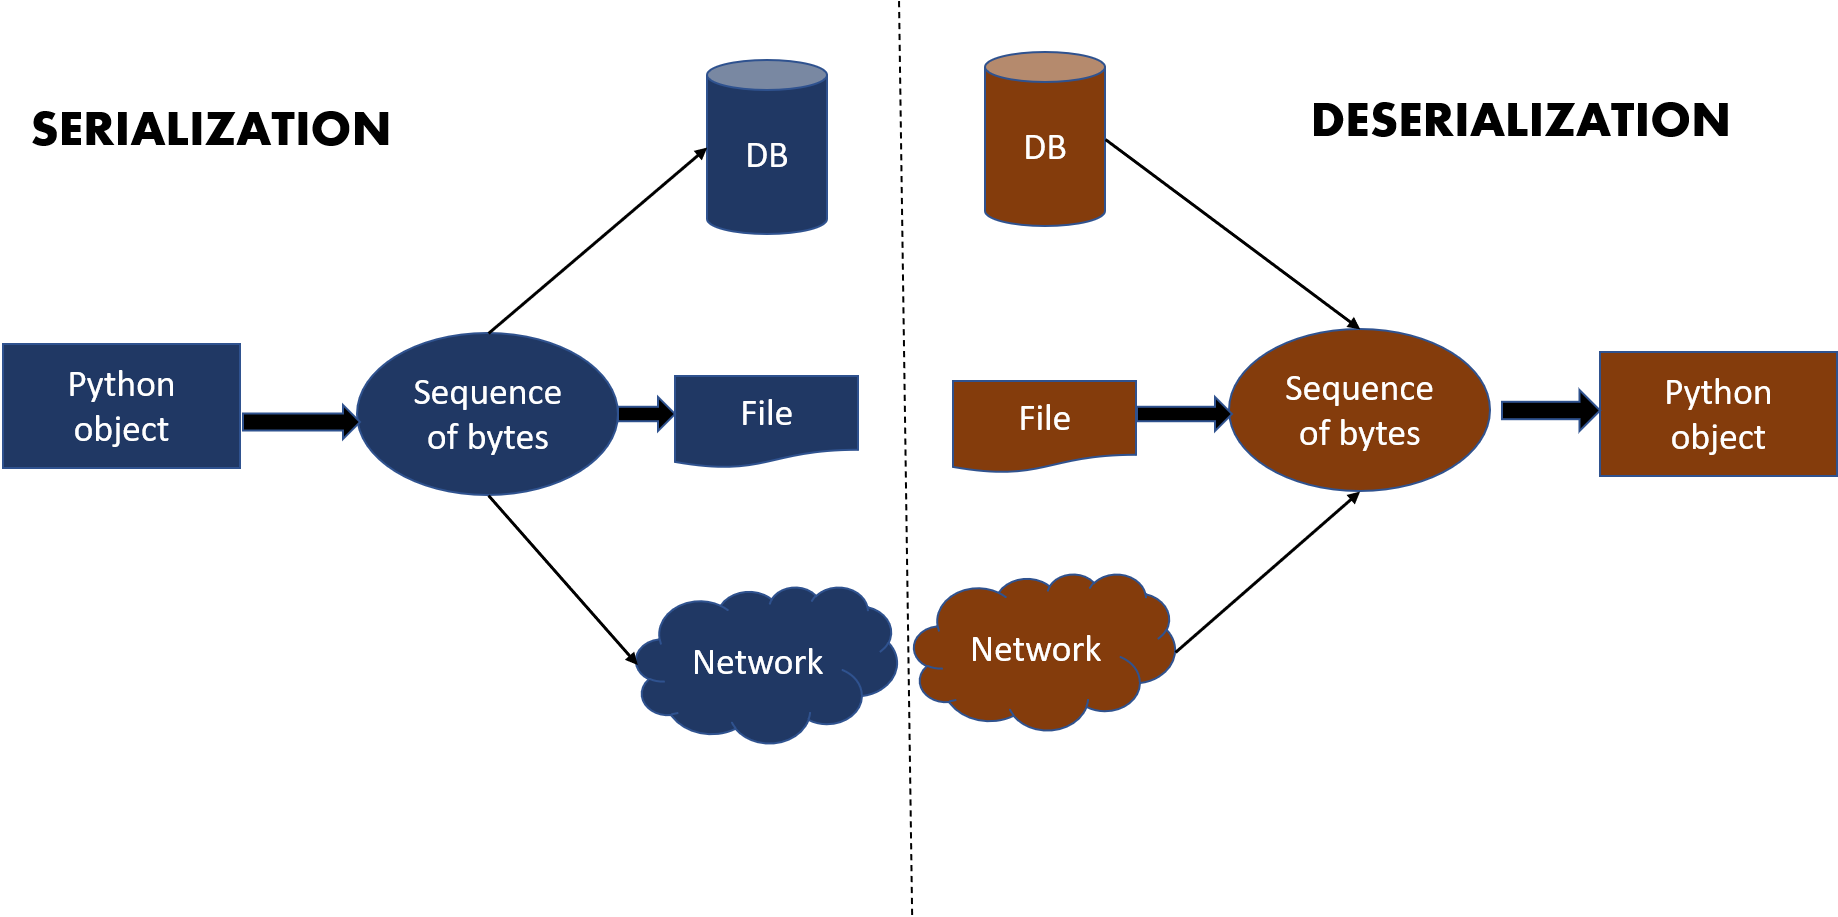
\includegraphics[width=0.8\textwidth]{images/serialization.png}
    \caption{(De)serialization}
    \label{fig:example-2}
\end{figure}

\newpage
\subsubsection{The \texttt{pickle} Module}
The \texttt{pickle} module provides functions for serializing and deserializing Python objects. It allows objects to be converted into a byte stream, which can then be saved to a file or transmitted over a network. The primary functions provided by the \texttt{pickle} module are:

\begin{itemize}
    \item \textbf{pickle.dump()}\\
    This function is used to serialize an object into a binary file. It takes two arguments: the object to be serialized and a file object (opened in binary write mode 'wb') to which the serialized data will be written. The function then writes the serialized data to the specified file, converting the object into a byte stream that can be saved to disk. Pickle is a module that provides serialization and deserialization functionalities.
    
    \item \textbf{pickle.load()}\\
    This function is used to deserialize an object from a binary file previously created using \texttt{pickle.dump()}. It takes a file object (opened in binary read mode 'rb') containing the serialized data as input and returns the deserialized object. The function reads the serialized data from the file and reconstructs the original object, effectively reversing the serialization process.
    
    \item \textbf{pickle.dumps()}\\
    This function is used to serialize an object into a byte stream representation, but it does \textbf{NOT write the data to a file}. Instead, it returns a byte string containing the serialized data.
    
    \item \textbf{pickle.loads()}\\
    This function is used to deserialize an object from a byte stream previously created using \texttt{pickle.dumps()}. It takes a byte string containing the serialized data as input and returns the deserialized object.
\end{itemize}



\begin{codebox}
\begin{minted}{python}
import pickle

class Fruit:
    def __init__(self, name: str, calories: float):
        self.name = name
        self.calories = calories
    
    def describe(self):
        print(self.name, self.calories, sep=': ')


# Create an instance of the Fruit class
banana: Fruit = Fruit('Banana', 100)

# Serialize the banana object and write it to the 'data.pickle' file
with open('data.pickle', 'wb') as file:
    pickle.dump(banana, file)
    
# Deserialize the object from the 'data.pickle' file
with open('data.pickle', 'rb') as file:
    fruit: Fruit = pickle.load(file)

fruit.describe() # Output: Banana: 100
\end{minted}
\end{codebox}


\newpage
The \texttt{pickle} module supports the serialization of various data types, including:

\begin{itemize}
    \item \textbf{Basic Data Types}\\
    Python's basic data types such as integers, floats, strings, and booleans can be easily serialized using the \texttt{pickle} module.
    
    \item \textbf{Lists, Tuples, and Dictionaries}\\
    Lists, tuples, and dictionaries, which are fundamental data structures, can also be serialized using \texttt{pickle}. This allows complex data structures to be stored and retrieved as a single object.
    
    \item \textbf{Custom Objects}\\
    Custom objects created by the user can also be serialized using \texttt{pickle}, provided that they are properly defined and their attributes are serializable. This allows entire object graphs to be stored and reconstructed later.
    
    \item \textbf{Functions and Classes}\\
    Functions and classes can be pickled as well, although there are limitations on what can be serialized. For instance, functions and classes defined at the top level of a module can typically be pickled, but dynamically created functions or classes may not be picklable.
\end{itemize}

\subsubsection{The \texttt{shelve} Module}
The \texttt{shelve} module provides a simple interface for managing persistent storage of Python objects. It allows you to store and retrieve objects from a file using key-value pairs, similar to a dictionary. It is particularly useful for applications that need to store data between program executions without requiring the complexity of a relational database.\\

\begin{codebox}
\begin{minted}{python}
import shelve

with shelve.open('TestDB') as db:
    db['one'] = 1
    db['two'] = 2
    db['three'] = 3

with shelve.open('TestDB') as db:
    print(type(db))
    print(dict(db))
    print(db['three'])
\end{minted}
\end{codebox}


\begin{minted}[
    bgcolor=white, % Background color
    frame=leftline, % Border style (only on left and right sides)
    framesep=2mm, % Padding around the frame
    rulecolor=black, % Border color
    linenos=false, % Disable line numbering
]{text}
<class 'shelve.DbfilenameShelf'>
{'one': 1, 'two': 2, 'three': 3}
3
\end{minted}

\textbf{Note}: The \texttt{shelve} module uses the \texttt{pickle} module internally for serializing and deserializing Python objects to and from the shelf file.

\newpage
\subsubsection{Storing Dictionaries with \texttt{shelve}}
This code defines a \texttt{Fruit} class with attributes for name and calories. It creates a dictionary of fruit objects and stores it persistently using the \texttt{shelve} module. 

\begin{codebox}
\begin{minted}{python}
import shelve

class Fruit:
    def __init__(self, name, calories):
        self.name = name
        self.calories = calories


data: dict = {
    'apple': Fruit('Apple', 10),
    'banana': Fruit('Banana', 100),
    'orange': Fruit('Orange', 50)
}

# Store fruits data
with shelve.open('FruitsDB') as db:
    db.update(data)
\end{minted}
\end{codebox}

\subsubsection{Retrieve Data from the shelf}
This code retrieves data from a persistent storage called a "shelf", specifically from a shelf file named \texttt{FruitsDB}.
\begin{codebox}
\begin{minted}{python}
import shelve

with shelve.open('FruitsDB') as db:
    # Retrieve the apple object
    apple: Fruit = db['apple']
        
    # Retrieve the banana object using the .get() method
    banana = db.get('banana')
    lemon = db.get('lemon')  # Returns None if the key does not exist
    
    # If key doesn't exist, it will add it with a default value of -1
    pomegranate = db.setdefault('pomegranate', -1)
    
    
# Prints the calories count of apple
print("Calories in an apple:", apple.calories)  # Output: 10
\end{minted}
\end{codebox}

%%%%%%%%%%%%%%%%%%%%%%%%%%%%%%%%%%%%%%%%%%%%%%%%%%%%%%%%%%%%%%%%%%%%%%%%%%
% 1.9
\newpage
\subsection{Exceptions}

\subsubsection{Errors}
Errors can be raised explicitly using the \texttt{raise} statement. This feature allows developers to generate exceptions when certain conditions are met, granting greater control over error handling within their code.

\begin{codebox}
\begin{minted}{python}
raise SomeException("Error message")
\end{minted}
\end{codebox}

\subsubsection{BaseException}
BaseException is the base class for all built-in exceptions. It serves as the superclass for all exceptions defined, including both system-defined exceptions (like ZeroDivisionError, TypeError, ValueError, etc.) and user-defined exceptions.

\begin{figure}[h!]
    \centering
    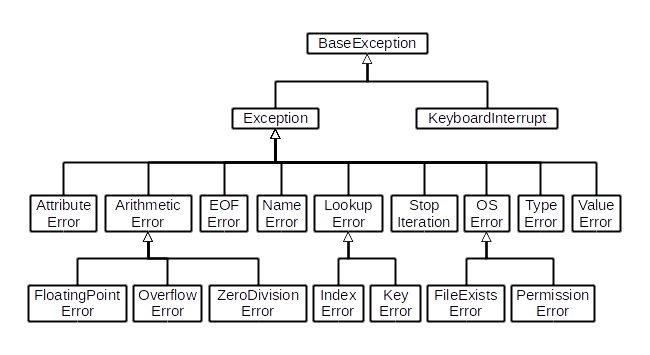
\includegraphics[width=0.95\textwidth]{images/exceptions.png}
    \caption{BaseException}
    \label{fig:example-3}
\end{figure}

\subsubsection{Exceptions as Objects}
In many programming languages, including Python, exceptions are represented as objects. An exception object encapsulates information about an exceptional event that has occurred during the execution of a program. This object typically contains details such as the type of exception, a message describing the error, and sometimes additional data relevant to the specific exception.

\newpage
\subsubsection{Exceptions}
Exceptions are used to handle errors and unexpected situations that may occur during the execution of a program. Using \texttt{try} and \texttt{except} blocks allows to handle errors, preventing the program from crashing and providing useful feedback to the user. It's a fundamental tool for writing robust and reliable code.
\begin{codebox}
\begin{minted}{python}
try:
    x = int(input("Please enter a number: "))
    result = 10 / x
    print("Result:", result)
    
except ZeroDivisionError:
    print("Error: Cannot divide by zero!")
    
except ValueError:
    print("Error: Please enter a valid number!")
\end{minted}
\end{codebox}

\begin{itemize}
    \item \textbf{\texttt{try:}} The \texttt{try} block contains the code that you want to execute. It is the part of the code where you anticipate an error might occur. If an exception occurs within this block, Python will stop executing the code in the \texttt{try} block and move to the \texttt{except} block.
    \item \textbf{\texttt{except:}} The \texttt{except} block is used to handle exceptions raised in the preceding \texttt{try} block. You can specify the type of exception you expect to occur. If the specified exception occurs in the \texttt{try} block, Python will execute the code in the \texttt{except} block.
\end{itemize}

\subsubsection{Named Attributes of Exception Objects}
Exception objects often have named attributes that provide information about the nature of the exception. These attributes can vary depending on the programming language and the specific exception type, but common attributes include:
\begin{itemize}
    \item \textbf{Type:} Indicates the type of exception that occurred. This could be a built-in exception type provided by the language or a custom exception type defined by the programmer.
    \item \textbf{Message:} A human-readable description of the error that occurred. This message often provides details about what went wrong and can be helpful for debugging.
    \item \textbf{Stack Trace:} A traceback or stack trace provides information about the sequence of function calls that led to the exceptional condition. It includes the file names, line numbers, and function names of the code where the exception occurred, helping developers pinpoint the source of the error.
    \item \textbf{Error Code:} Some exceptions may include an error code that provides additional context or categorization for the error.
    \item \textbf{Additional Data:} Depending on the exception type and the needs of the programmer, exception objects may contain additional data relevant to the exceptional condition. This could include input values, state information, or any other details that might be useful for handling the exception.
\end{itemize}

\subsubsection{Custom Exceptions}
Custom exceptions can be created to handle specific cases that are not covered by built-in exceptions.
\begin{codebox}
\begin{minted}{python}
# Custom exception class by inheriting from the built-in Exception class
class CustomException(Exception):
    def __init__(self, message="An error occurred"):
        self.message = message
        super().__init__(self.message)

# Example function that raises the custom exception
def example_function(number):
    if number < 0:
        # Raise the custom exception if the input is negative
        raise CustomException("Number cannot be negative")

try:
    # Call function with a negative number to trigger the custom exception
    example_function(-5)
except CustomException as e:
    # Handle the custom exception
    print("Custom Exception Caught:", e.message)
\end{minted}
\end{codebox}

\subsubsection{Chained Exceptions}
Chained exceptions, also known as nested exceptions or exception chaining, refer to the practice of capturing and preserving information about one exception while throwing another. This mechanism is particularly useful in scenarios where an error occurs within the context of handling another error.

Many modern programming languages and frameworks support chaining exceptions directly in their exception handling mechanisms. For example you can chain exceptions using the \texttt{raise} statement with the \texttt{from} keyword:

\begin{codebox}
\begin{minted}{python}
try:
    # Code that may raise Exception A
    raise Exception("Exception A occurred")
except Exception as e:
    try:
        # Code that may raise Exception B
        raise ValueError("Exception B occurred") from e
    except ValueError as ve:
        # Handle or re-raise Exception B
        print("Caught ValueError:", ve)
\end{minted}
\end{codebox}

In the above example, Exception B is raised with Exception A chained to it using the \texttt{from} keyword. This preserves the traceback information of Exception A while raising Exception B.

Chained exceptions are beneficial for understanding the flow of errors in a program and can greatly assist in debugging complex systems. However, it's essential to use them judiciously and avoid excessive nesting, which can make the code harder to follow.

\newpage
\subsubsection{The \texttt{\_\_cause\_\_} and \texttt{\_\_context\_\_} Attributes}
The \texttt{\_\_cause\_\_} and \texttt{\_\_context\_\_} are attributes of the exception object (\texttt{ve} in this case) that provide information about the relationships between exceptions.

\begin{itemize}
    \item \textbf{\texttt{\_\_cause\_\_}}: This attribute refers to the exception that caused the current exception to occur. It is used to indicate that the current exception was raised in direct response to another exception. In the given code, \texttt{ve.\_\_cause\_\_} prints the original exception (\texttt{Exception A}) that caused the \texttt{ValueError} exception (\texttt{Exception B}) to be raised.
    
    \item \textbf{\texttt{\_\_context\_\_}}: This attribute refers to the exception that was being handled when the current exception was raised. It provides context for the current exception. In the given code, \texttt{ve.\_\_context\_\_} would print \texttt{None} because there's no explicitly defined context for the \texttt{ValueError} exception. If there were an outer \texttt{except} block handling another exception, the exception object from that outer block would be accessible via \texttt{\_\_context\_\_}.
\end{itemize}


\begin{codebox}
\begin{minted}{python}
try:
    # Code that may raise Exception A
    raise Exception("Exception A occurred")
except Exception as e:
    try:
        # Code that may raise Exception B
        raise ValueError("Exception B occurred") from e
    except ValueError as ve:
        # Handle or re-raise Exception B
        print("Caught ValueError:", ve)
        print(ve.__cause__)
        print(ve.__context__)
\end{minted}
\end{codebox}


\begin{minted}[
    bgcolor=white, % Background color
    frame=leftline, % Border style (only on left and right sides)
    framesep=2mm, % Padding around the frame
    rulecolor=black, % Border color
    linenos=false, % Disable line numbering
]{text}
Caught ValueError: Exception B occurred
Exception A occurred
Exception A occurred
\end{minted}

\subsubsection{Implicitly and Explicitly Chained Exceptions}
Chained exceptions, both implicit and explicit, provide a way to maintain a history of exceptions that have occurred during program execution. This feature helps developers to debug and understand the flow of exceptions in their code more effectively.

\begin{itemize}
\item \textbf{Implicitly Chained Exceptions}\\ Implicitly chained exceptions occur when an exception is raised within the except block without explicitly specifying the original exception as the cause. In this case, Python automatically chains the new exception to the original one.
\item \textbf{Explicitly Chained Exceptions}\\
You can explicitly raise a new exception while capturing the original exception to provide more context. This is done using the \texttt{raise ... from ...} syntax. 
\end{itemize}

\newpage
\subsubsection{The \texttt{\_\_traceback\_\_} Attribute}
The \texttt{\_\_traceback\_\_} attribute of an exception object contains the traceback information associated with that exception. The traceback provides a detailed record of the execution path that led to the exception, including the sequence of function calls and the line numbers where the exception occurred.

\begin{codebox}
\begin{minted}{python}
import traceback

def function_with_error():
    # Some code that may raise an exception
    raise ValueError("An error occurred in function_with_error")

try:
    function_with_error()
except ValueError as e:
    # Accessing the __traceback__ attribute
    tb = e.__traceback__
    # Printing the traceback using the traceback module
    print(traceback.format_tb(tb))
\end{minted}
\end{codebox}

The traceback module provides functions to work with traceback objects.

\begin{itemize}
    \item \texttt{traceback.print\_tb(tb)}: Prints the traceback information to the standard output.
    \item \texttt{traceback.format\_tb(tb)}: Returns a formatted string containing traceback information.
    \item \texttt{traceback.extract\_tb(tb)}: Returns a list of tuples representing traceback information. Each tuple contains filename, line number, function name, and source line.
\end{itemize}

\subsubsection{Operating with different kinds of Exceptions}
The code efficiently handles potential errors by incorporating separate blocks for different types of exceptions, ensuring readability through clear separation and descriptive comments. Additionally, it adheres to Python's PEP 8 style guide for code layout, enhancing overall clarity and maintainability.
\begin{codebox}
\begin{minted}{python}
try:
    # Your code that may raise exceptions
    x = int(input("Enter a number: "))
    y = 10 / x
    print("Result:", y)

except ValueError:
    # Handle ValueError (invalid input)
    print("Please enter a valid integer.")

except ZeroDivisionError:
    # Handle ZeroDivisionError (division by zero)
    print("Cannot divide by zero.")

except Exception as e:
    # Catch any other unexpected exceptions
    print("An error occurred:", e)
\end{minted}
\end{codebox}







\section{Coding Conventions, Best Practices, and Standarization}

\subsection{PEPs}

\href{https://peps.python.org/}{Python Enhancement Proposals (PEPs)} is an online document, which is a collection of guidelines, best practices, descriptions of (new) features and implementations, as well as processes, mechanisms and important information surrounding Python. There are many PEPs, hundreds of them.

\begin{itemize}
    \item \textbf{\href{https://www.python.org/dev/peps/}{PEP 0 - Index of Python Enhancement Proposals (PEPs)}}
    \item \textbf{\href{https://www.python.org/dev/peps/pep-0001/}{PEP 1 - PEP Purpose and Guidelines:} Information about the purpose of PEPs, their types, and introduces general guidelines}
    \item \textbf{\href{https://www.python.org/dev/peps/pep-0008/}{PEP 8 - Style Guide for Python Code:} Conventions and best practices for Python coding}
    \item \textbf{\href{https://www.python.org/dev/peps/pep-0020/}{PEP 20 - The Zen of Python:} List of principles for Python’s design}
    \item \textbf{\href{https://www.python.org/dev/peps/pep-0257/}{PEP 257 - Docstring Conventions:} Provides guidelines for conventions and semantics associated with Python docstrings}
    \item \textbf{\href{https://www.python.org/dev/peps/pep-0484/}{PEP 484 - Type Hints:} Introduces a syntax for specifying type annotations in Python code}
\end{itemize}

\newpage
\subsection{PEP 1 – PEP Purpose and Guidelines}
\subsubsection{What is a PEP?}
PEP stands for Python Enhancement Proposal. A PEP is a design document providing information to the Python community, or describing a new feature for Python or its processes or environment. The PEP should provide a concise technical specification of the feature and a rationale for the feature. We intend PEPs to be the primary mechanisms for proposing major new features, for collecting community input on an issue, and for documenting the design decisions that have gone into Python. The PEP author is responsible for building consensus within the community and documenting dissenting opinions.

Because the PEPs are maintained as text files in a versioned repository, their revision history is the historical record of the feature proposal. This historical record is available by the normal git commands for retrieving older revisions, and can also be browsed on GitHub.\\

\subsubsection{PEP Audience}
The typical primary audience for PEPs are the core developers of the CPython reference interpreter and their elected Steering Council, as well as developers of other implementations of the Python language specification.

However, other parts of the Python community may also choose to use the process (particularly for Informational PEPs) to document expected API conventions and to manage complex design coordination problems that require collaboration across multiple projects.\\

\subsubsection{PEP Types}
There are three kinds of PEP:

\begin{itemize}
    \item \textbf{Standards Track PEP:} Describes a new feature or implementation for Python. It may also describe an interoperability standard that will be supported outside the standard library for current Python versions before a subsequent PEP adds standard library support in a future version.
    
    \item \textbf{Informational PEP:} Describes a Python design issue, or provides general guidelines or information to the Python community, but does not propose a new feature. Informational PEPs do not necessarily represent a Python community consensus or recommendation, so users and implementers are free to ignore Informational PEPs or follow their advice.
    
    \item \textbf{Process PEP:} Describes a process surrounding Python, or proposes a change to (or an event in) a process. Process PEPs are like Standards Track PEPs but apply to areas other than the Python language itself. They may propose an implementation, but not to Python’s codebase; they often require community consensus; unlike Informational PEPs, they are more than recommendations, and users are typically not free to ignore them. Examples include procedures, guidelines, changes to the decision-making process, and changes to the tools or environment used in Python development. Any meta-PEP is also considered a Process PEP.
\end{itemize}

\newpage
\subsection{PEP 8 – Style Guide for Python Code}

PEP 8 is a guide for writing Python code that enhances its readability and maintainability. It provides guidelines for formatting, naming conventions, code structure, and documentation.

Code is read much more often than it is written. The guidelines provided here are intended to improve the readability of code and make it consistent across the wide spectrum of Python code. As PEP 20 says, “Readability counts”.\\

\subsubsection{Key Points from PEP 8}

\begin{itemize}
    \item \textbf{Indentation:} Use 4 spaces per indentation level. Spaces are the preferred indentation method. Tabs should be used solely to remain consistent with code that is already indented with tabs. Python disallows mixing tabs and spaces for indentation.
    \item \textbf{Line Length:} Limit lines to 79 characters to enhance readability. For flowing long blocks of text with fewer structural restrictions (docstrings or comments), the line length should be limited to 72 characters.
    \item \textbf{Blank Lines:} Use blank lines to separate functions, classes, and sections of code logically.
    \item \textbf{Imports:} Import statements should be on separate lines and grouped in the following order: standard library imports, related third-party imports, and local application/library specific imports.
    \item \textbf{Whitespace:} Use whitespace to improve readability, but avoid excessive use.
    \item \textbf{Naming Conventions:} Follow naming conventions for variables, functions, and classes to maintain consistency.
    \item \textbf{Comments:} Write comments to explain non-obvious code, but avoid redundant comments.
    \item \textbf{Docstrings:} Use docstrings to document modules, functions, classes, and methods.
    \item \textbf{Coding Recommendations:} Follow best practices for coding, such as using exception handling properly and preferring exceptions to returning \texttt{None}.
    \item \textbf{Version Bookkeeping:} Use \texttt{\_\_version\_\_} for version information in modules.
        \item \textbf{Line Break Before or After Binary Operator:} It is permissible to break before or after a binary operator, as long as the convention is consistent locally. For new code it is suggested, where a line break occurs before binary operators for improved readability.
    \item \textbf{String Quotes:} Single-quoted strings and double-quoted strings are the same. This PEP does not make a recommendation for this. Pick a rule and stick to it. When a string contains single or double quote characters, however, use the other one to avoid backslashes in the string. It improves readability.
    \item \textbf{Line Continuation:} If implicit line continuation is not possible, such as when breaking a long string or expression outside of parentheses, you can use a backslash at the end of the line to indicate that it continues on the next line.
\end{itemize}

\newpage
\subsubsection{Naming Conventions}
Following naming conventions is essential for writing clean, readable, and maintainable code. Following naming conventions helps make your Python code more consistent and understandable for yourself and others who may read or work with your code.

\begin{itemize}
    \item \textbf{Variables and function names}
    \begin{itemize}
        \item Use \textbf{snake\_case}, lowercase letters with words separated by underscores for variable names and function names.
        \item Example: \texttt{my\_variable}, \texttt{calculate\_average()}
    \end{itemize}

    \item \textbf{Constants}
    \begin{itemize}
        \item Use \textbf{SCREAMING\_SNAKE\_CASE}, uppercase letters with words separated by underscores for constant names.
        \item Example: \texttt{MAX\_VALUE}, \texttt{PI}
    \end{itemize}

    \item \textbf{Class names}
    \begin{itemize}
        \item Use \textbf{CamelCase} for class names, starting with an uppercase letter.
        \item Example: \texttt{MyClass}, \texttt{Person}
    \end{itemize}

    \item \textbf{Package and module names}
    \begin{itemize}
         \item Use lowercase letters for package and module names, avoiding underscores if possible.
        \item Example: \texttt{mypackage}, \texttt{my\_module}, \texttt{utilities}, \texttt{data\_processing}
    \end{itemize}

 
\end{itemize}

\begin{figure}[h!]
    \centering
    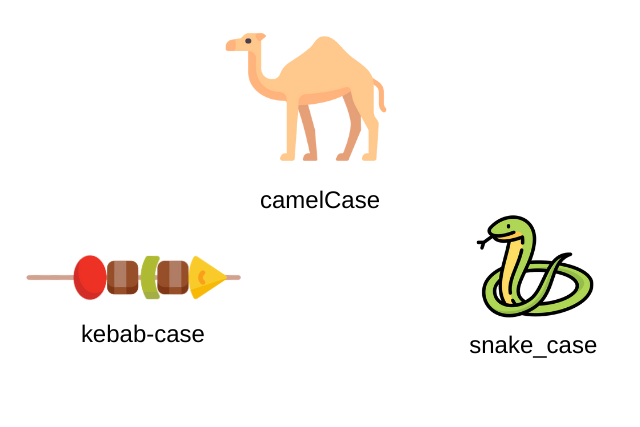
\includegraphics[width=0.6\textwidth]{images/cases2.png}
    \caption{Cases}
    \label{fig:cc-1}
\end{figure}

\newpage
\subsubsection{Comments}
\textbf{Block Comments}\\
Block comments generally apply to some (or all) code that follows them, and are indented to the same level as that code. Each line of a block comment starts with a comment marker \texttt{\#} and a single space, unless it is indented text inside the comment. Paragraphs inside a block comment are separated by a line containing a single comment marker.\\

\begin{codebox}
\begin{minted}{python}
# This is a block comment
# This function calculates the area of a circle.
# It takes the radius of the circle as input and returns the calculated area.
def calculate_area(radius):
    pi = 3.14159
    area = pi * radius ** 2
    return area
\end{minted}
\end{codebox}


\spacedtextbf{Inline comments}
\begin{itemize}
\item Use inline comments sparingly.
\item An inline comment is a comment on the same line as a statement. 
\item Should be separated by at least two spaces from the statement. 
\item They should start with a \texttt{\#} and a single space.
\item Inline comments are unnecessary and in fact distracting if they state the obvious.
\end{itemize}
%\begin{codebox}
%\begin{minted}{python}
%x = x + 1   # Increment x
%\end{minted}
%\end{codebox}


\subsubsection{Compliant Checker}
A PEP8 compliant checker is a tool used to ensure that Python code conforms to the guidelines outlined in PEP8, which is the Python Enhancement Proposal that provides conventions for writing Python code in a consistent and readable manner. PEP8 covers aspects such as indentation, line length, import formatting, naming conventions, and more.

There are several tools available for checking PEP8 compliance of Python code, including:

\begin{itemize}
    \item \textbf{pycodestyle}: Formerly known as pep8, this is a tool to check Python code against the PEP8 style guide. It can be run from the command line.
    
    \item \textbf{flake8}: Combines several tools in one package, including pycodestyle, pyflakes (for static code analysis), and McCabe (for complexity checking). It provides a comprehensive tool for checking both PEP8 compliance and potential errors in your code.
    
    \item \textbf{Black}: While not strictly a PEP8 checker, Black is a code formatter that automatically reformats Python code to comply with PEP8 standards. It enforces a consistent style by rewriting code to adhere to its strict rules.
    
    \item \textbf{PyLint}: Another popular tool for analyzing Python code for errors, it also provides checks for PEP8 compliance among other things.
\end{itemize}

\newpage
\subsection{PEP 20 – The Zen of Python}

PEP 20 is titled "The Zen of Python" and was authored by Tim Peters. It serves as a set of guiding principles or philosophies for the design of the Python programming language. It encapsulates the core values and ideals that Python's creators and community strive to uphold in their programming practices. The aphorisms, or principles, outlined in PEP 20 are:\\

\begin{itemize}
    \item Beautiful is better than ugly.
    \item Explicit is better than implicit.
    \item Simple is better than complex.
    \item Complex is better than complicated.
    \item Flat is better than nested.
    \item Sparse is better than dense.
    \item Readability counts.
    \item Special cases aren't special enough to break the rules.
    \item Although practicality beats purity.
    \item Errors should never pass silently.
    \item Unless explicitly silenced.
    \item In the face of ambiguity, refuse the temptation to guess.
    \item There should be one-- and preferably only one --obvious way to do it.
    \item Although that way may not be obvious at first unless you're Dutch.
    \item Now is better than never.
    \item Although never is often better than \textit{right} now.
    \item If the implementation is hard to explain, it's a bad idea.
    \item If the implementation is easy to explain, it may be a good idea.
    \item Namespaces are one honking great idea -- let's do more of those!
\end{itemize}

\subsubsection{Easter Egg: \texttt{import this}}
The term "Easter Egg" refers to a hidden feature or message that developers embed within the code for amusement or as a tribute. The term is derived from the tradition of hiding Easter eggs for children to find during Easter egg hunts.\\

The code snippet "\texttt{import this}" is a well-known Easter Egg. When executed in a Python interpreter, it displays "The Zen of Python," which is a collection of aphorisms that capture the guiding principles of Python's design philosophy. These aphorisms were written by Tim Peters, and they provide insights into the mindset and values of Python developers.

%\begin{figure}[h]
%    \centering
%    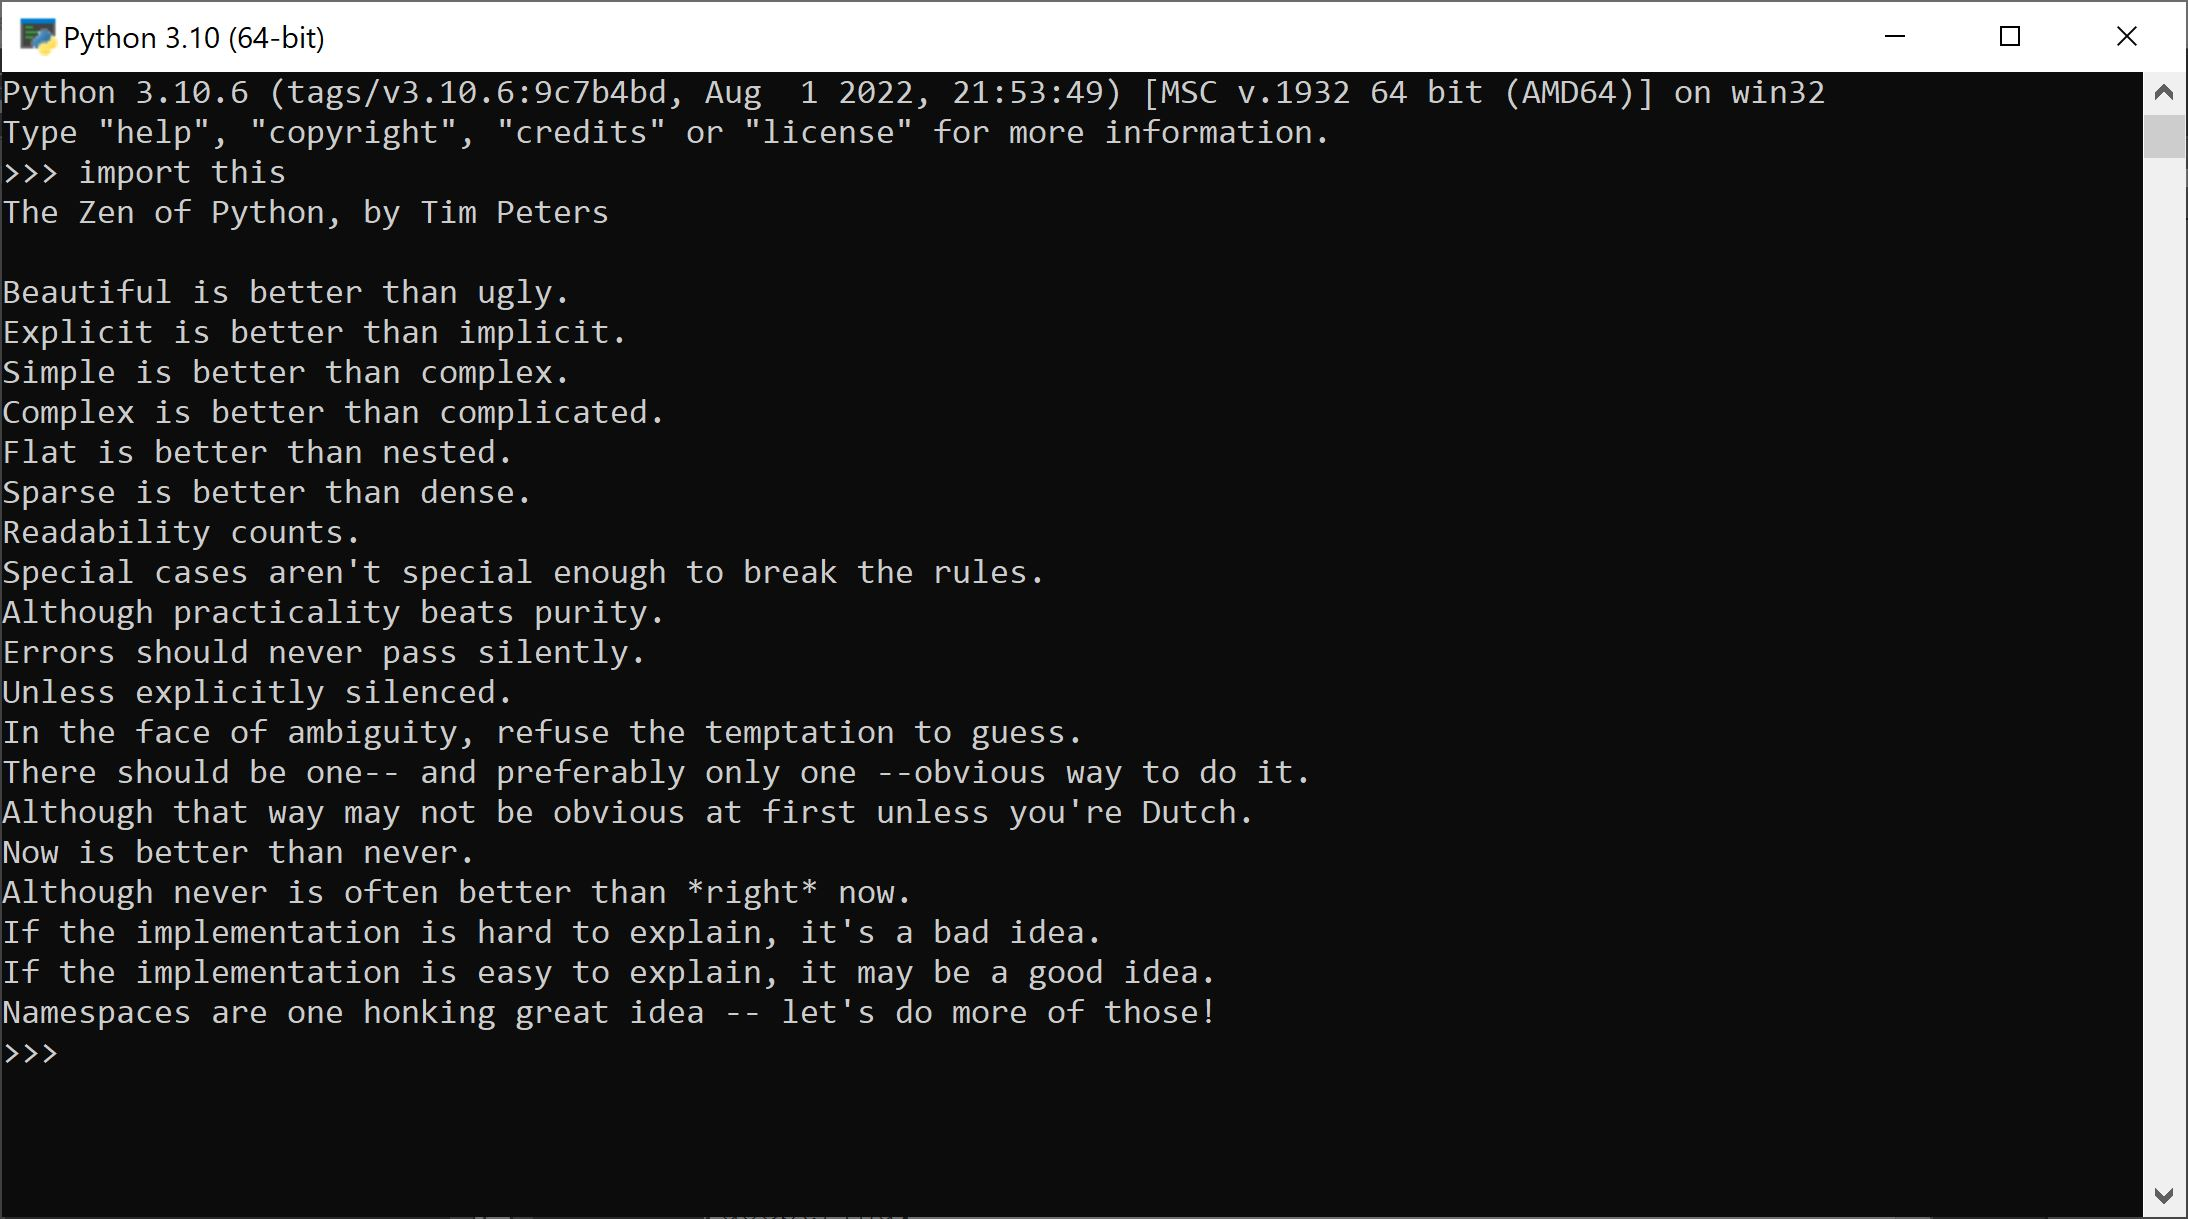
\includegraphics[width=\textwidth]{images/import_this.JPG}
%    \caption{import this}
%    \label{fig:example}
%\end{figure}

\newpage
\subsection{PEP 257 – Docstring Conventions}
PEP 257 provides conventions for writing docstrings. Docstrings are documentation strings that appear as the first statement in a module, function, class, or method definition. The key points from PEP 257 are:

\begin{itemize}
    \item Docstrings should be enclosed in triple quotes, e.g. \texttt{"""This is a docstring."""}.
    \item For a multi-line docstring, the opening and closing quotes should be on separate lines.
    \item The first line of a docstring should be a summary of the object's purpose, starting with a capital letter and ending with a period.
    \item If the docstring has multiple paragraphs, subsequent paragraphs should be separated by a blank line.
    \item Docstrings should be written in complete sentences and follow proper grammar and punctuation rules.
    \item Docstrings should include information about the function or method's parameters, return values, exceptions raised, and any side effects.
    \item For module-level docstrings, they should include an overview of the module's contents and usage examples.
    \item For class docstrings, they should describe the class's purpose, behavior, and usage, including information about constructor arguments and instance variables.
\end{itemize}

\subsubsection{One-line Docstrings}
One-liners are for really obvious cases. They should really fit on one line.
\begin{codebox}
\begin{minted}{python}
def kos_root():
    """Return the pathname of the KOS root directory."""
    global _kos_root
    if _kos_root: return _kos_root
    ...
\end{minted}
\end{codebox}

\begin{itemize}
    \item Triple quotes are used even though the string fits on one line. Makes it easy to expand it.
    \item The closing quotes are on the same line as the opening quotes. Looks better for one-liners.
    \item There’s no blank line either before or after the docstring.
    \item The docstring is a phrase ending in a period. It prescribes the function or method’s effect as a command (“Do this”, “Return that”), not as a description; e.g. don’t write “Returns the pathname …”.
    \item The one-line docstring should NOT be a “signature” reiterating the function/method parameters (which can be obtained by introspection).
\end{itemize}

\newpage
\subsubsection{Multi-line Docstrings}
Multi-line docstrings consist of a summary line just like a one-line docstring, followed by a blank line, followed by a more elaborate description. The summary line may be used by automatic indexing tools; it is important that it fits on one line and is separated from the rest of the docstring by a blank line. The summary line may be on the same line as the opening quotes or on the next line. The entire docstring is indented the same as the quotes at its first line (see example below).
\begin{codebox}
\begin{minted}{python}
def complex(real=0.0, imag=0.0):
    """Form a complex number.

    Keyword arguments:
    real -- the real part (default 0.0)
    imag -- the imaginary part (default 0.0)
    """
    if imag == 0.0 and real == 0.0:
        return complex_zero
    ...
\end{minted}
\end{codebox}

\subsubsection{Linters and Fixers}
Linters and fixers are tools used in software development to analyze source code for potential errors, bugs, stylistic inconsistencies, and adherence to coding standards. They automate the process of code review by identifying issues and providing feedback to developers, helping ensure code quality, consistency, and maintainability.\\

\begin{itemize}
\item \textbf{Linter}
\begin{itemize}
    \item Static code analysis tool used to flag programming errors, bugs, stylistic errors, and suspicious constructs in the source code without actually executing it.
    \item Maintain a consistent coding style within a project and can catch common programming mistakes early in the development process.
    \item Commonly used in software development to improve code quality, readability, and maintainability.
\end{itemize}

\item \textbf{Fixer}
\begin{itemize}
    \item Tool that automatically corrects or adjusts code based on the suggestions and warnings provided by a linter.
    \item Automatically apply changes to the code, such as formatting corrections, removing unused imports, or fixing syntax errors.
    \item Streamline the development process by automating repetitive tasks and ensuring that the codebase adheres to the defined coding standards.
\end{itemize}
\end{itemize}


\newpage
\subsection{PEP 484 – Type Hints}
In Python, "types" refer to the classification of data into different categories, such as integers, strings, lists, etc. Python is known for its dynamic typing system, which means that the type of a variable is inferred at runtime based on the value it holds. This is in contrast to statically typed languages like Java or C++, where you must declare the type of a variable explicitly.

\subsubsection{Dynamic Typing}
Python's dynamic typing offers flexibility and simplicity, allowing developers to write code more quickly and concisely. However, it also means that type errors may only be discovered at runtime, leading to potential bugs that can be harder to catch during development.\\

To address this issue, Python introduced optional static typing through PEP 483 and PEP 484. These proposals introduced type hints, a syntax for annotating variables, function parameters, and return values with their expected types. 
%Although these annotations are not enforced by the Python interpreter at runtime, they can be used by static analysis tools, such as MyPy, to perform type checking and catch potential errors early in the development process.

\begin{codebox}
\begin{minted}{python}
# Import the typing module for type hints
from typing import List

# Type hints for variables
age: int = 30
names: List[str] = ["Alice", "Bob", "Charlie"]

# Functions with type hints for parameters and return value
def greet(name: str) -> str:
    return f"Hello, {name}"

def upper_everything(elements: list[str]) -> list[str]:
    return [el.upper() for el in elements]
\end{minted}
\end{codebox}

\subsubsection{Type Checker: Mypy}
Mypy is an optional static type checker for Python that aims to combine the benefits of dynamic (or "duck") typing and static typing. Mypy combines the expressive power and convenience of Python with a powerful type system and compile-time type checking. Mypy type checks standard Python programs; run them using any Python VM with basically no runtime overhead.\\

Using mypy alongside your Python development workflow can help catch type-related errors early, improve code maintainability, and enhance collaboration, especially in larger projects or teams where type clarity is beneficial.

\begin{codebox}
\begin{minted}{bash}
# Install mypy
pip install mypy

# Run mypy on a single Python script or module
mypy your_script.py

# Run mypy on an entire directory (recursively)
mypy your_directory/
\end{minted}
\end{codebox}


\section{GUI Programming}

\subsection{Graphical User Interface (GUI)}
A GUI, pronounced as "gooey", stands for Graphical User Interface. The primary rationale behind GUIs is to enhance user experience by providing visual representations of program functions and data. GUIs enable users to interact with software applications through graphical elements like windows, buttons, menus, and icons, rather than relying solely on text-based commands.

GUI programming involves creating visually appealing interfaces for software applications using graphical elements like windows, buttons, and menus. Understanding basic GUI concepts and terminology is essential for developing user-friendly and intuitive applications.

\subsubsection{Visual Programming}
Visual programming involves creating applications using graphical elements rather than writing code manually. Examples of visual programming environments include Scratch, Blockly, and LabVIEW. These environments typically provide drag-and-drop interfaces for building applications, making it easier for users to create software without extensive programming knowledge.

\subsubsection{Widgets Toolkits}
Widget toolkits, also known as \textbf{GUI toolkits} or \textbf{frameworks}, provide libraries of reusable graphical components ("widgets") for building GUI applications. These toolkits offer APIs (Application Programming Interfaces) for creating and managing GUI elements, handling user interactions, and rendering graphical content. Examples of popular widget toolkits include Tkinter (for Python), Swing (for Java), WinForms (for .NET), and Qt (for C++ and Python).\\

\textbf{Widgets}, also known as controls, are graphical elements used in GUIs to interact with users or display information. Some basic terms associated with widgets include:

\begin{itemize}
    \item \textbf{Windows:} Rectangular areas on the screen that contain application content and controls.
    \item \textbf{Title and Title Bars:} The title of a window and the bar across the top of a window that contains the title and control buttons (minimize, maximize, close).
    \item \textbf{Buttons:} Controls that trigger actions when clicked, such as submitting a form or closing a window.
    \item \textbf{Icons:} Small graphical representations of files, folders, or applications.
    \item \textbf{Labels:} Text elements used to display static text or descriptions.
\end{itemize}

\subsubsection{Classical vs. Event-Driven Programming}
In classical programming, applications follow a sequential flow where each instruction is executed in order. In contrast, event-driven programming relies on events triggered by user actions or system events. Applications respond to these events by executing specific event-handling code. GUI programming is primarily event-driven, where user interactions such as clicking a button or typing in a text box trigger events that drive application behavior.\\

\textbf{Events} are actions or occurrences that happen during program execution, such as clicking a button, pressing a key, or moving the mouse. GUI applications respond to these events by executing event-handling code associated with each event type. Examples of events include mouse clicks, key presses, window resizing, and timer expiration.

\subsection{Tkinter}

\subsubsection{Simple Tkinter Application}
Tkinter is a Python library for creating GUI applications. It is the standard GUI toolkit for Python and is included with most Python installations, making it readily available for developers. Tkinter is based on the Tk GUI toolkit originally developed for the Tcl programming language.

\begin{codebox}
\begin{minted}{python}
import tkinter as tk

# Function to close the window
def close_window():
    root.destroy()

# Create the main Tkinter window
root = tk.Tk()
root.title("Simple Tkinter Application")

# Create a label widget
label = tk.Label(root, text="Hello, Tkinter!")
label.pack(pady=10)

# Create a button widget
close_button = tk.Button(root, text="Close", command=close_window)
close_button.pack()

# Start the Tkinter event loop
root.mainloop()
\end{minted}
\end{codebox}

\begin{figure}[h]
    \centering
    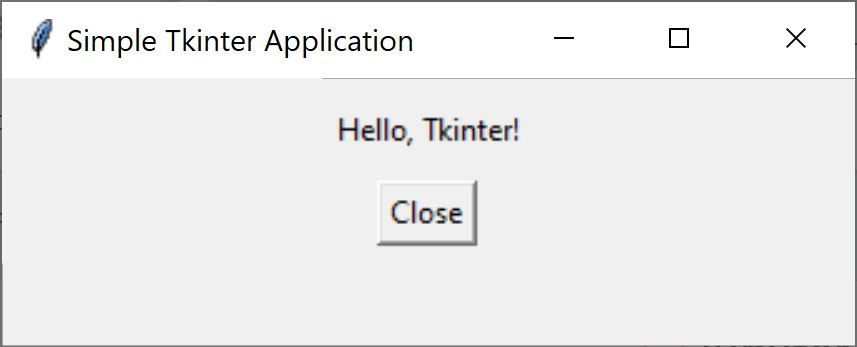
\includegraphics[width=0.6\textwidth]{images/tkinter1.JPG}
    \caption{Simple Tkinter Application}
    \label{fig:example}
\end{figure}

\subsubsection{The \texttt{mainloop()}}
In Tkinter, \texttt{mainloop()} is a method that runs an event loop, which listens for events such as user input (like mouse clicks and key presses) and system events. It's a fundamental part of any Tkinter application as it keeps the application running and responsive to user interactions.

\newpage
\subsubsection{Tkinter Widgets}

A widget is a graphical element or control used to display information or receive input in a GUI.

\begin{itemize}
    \item \textbf{Frame}: A container widget used to organize other widgets.
    
    \item \textbf{Label}: Displays text or images.
    
    \item \textbf{Button}: Generates an event when clicked.
    
    \item \textbf{Checkbutton}: Represents an on/off choice.
    
    \item \textbf{Radiobutton}: Allows the user to select one option from several.
    
    \item \textbf{Entry}: Accepts single-line text input from the user.
    
    \item \textbf{Combobox}: A combination of an Entry widget and a drop-down list.
    
    \item \textbf{Listbox}: Displays a list of items for selection.
    
    \item \textbf{Scrollbar}: Allows scrolling through content in widgets like Listbox or Canvas.
    
    \item \textbf{Sizegrip}: Provides a resize handle for resizable windows.
    
    \item \textbf{Text}: Multiline text editor.
    
    \item \textbf{Progressbar}: Displays the progress of a task.
    
    \item \textbf{Scale}: Represents a range of values as a slider.
    
    \item \textbf{Spinbox}: Input field with up/down buttons for numeric values.
    
    \item \textbf{Separator}: Horizontal or vertical line used to separate widgets.
    
    \item \textbf{Labelframe}: A frame with a title.
    
    \item \textbf{Panedwindow}: A container widget that holds panes (subwindows) split by a separator.
    
    \item \textbf{Notebook}: A tabbed notebook-like widget.
    
    \item \textbf{Canvas}: A drawing area for creating graphics and plots.
    
    \item \textbf{Treeview}: Displays hierarchical data in a tree-like structure.
\end{itemize}

\subsubsection{Widget Constructors}
A widget constructor is a method or function used to create an instance of a GUI component, typically known as a widget.

In frameworks like Tkinter (Python), JavaFX (Java), or PyQt (Python), GUI components like buttons, labels, text fields, etc., are created by calling specific constructor functions or methods provided by the framework. These constructor functions usually take parameters that define the initial properties or attributes of the widget, such as its size, position, text, color, etc. For example, in Tkinter, you might use the \texttt{Button} constructor to create a button widget.

\begin{codebox}
\begin{minted}{python}
import tkinter as tk

root = tk.Tk()

# Create a Button using the Button constructor
button = tk.Button(root, text="Click me", bg="red")

button.pack()

root.mainloop()
\end{minted}
\end{codebox}

\newpage
\subsubsection{Widget Properties and Methods}
Widget properties and methods provide essential functionalities for customizing and interacting with GUI elements in Tkinter.


\begin{itemize}
    \item \textbf{Common Properties}
    \begin{itemize}[label={--}]
        \item \texttt{text:} Sets or retrieves the text displayed by the widget.
        \item \texttt{bg:} Sets or retrieves the background color of the widget.
        \item \texttt{fg:} Sets or retrieves the foreground (text) color of the widget.
        \item \texttt{font:} Sets or retrieves the font used for the text in the widget.
        \item \texttt{width:} Sets or retrieves the width of the widget.
        \item \texttt{height:} Sets or retrieves the height of the widget.
        \item \texttt{state:} Sets or retrieves the state of the widget (normal, disabled, etc.).
        \item \texttt{variable:} Sets or retrieves the associated Tkinter variable.
    \end{itemize}

    \item \textbf{Common Methods}
    \begin{itemize}[label={--}]
        \item \texttt{config(**options):} Configures one or more widget options.
        \item \texttt{grid(**options):} Places the widget in the parent widget using a grid layout.
        \item \texttt{pack(**options):} Packs the widget into the parent widget.
        \item \texttt{place(**options):} Places the widget in the parent widget using absolute positioning.
        \item \texttt{focus():} Sets the keyboard focus to the widget.
        \item \texttt{bind(event, handler):} Binds an event to a handler function.
        \item \texttt{destroy():} Destroys the widget and removes it from the display.
    \end{itemize}
\end{itemize}


\newpage
\subsubsection{Positioning Widgets: \texttt{pack()} and \texttt{place()} and \texttt{grid()}}

In Tkinter, you can use various geometry managers to position widgets within a window. The most commonly used managers are \texttt{pack()}, \texttt{place()}, and \texttt{grid()}. If you want to position widgets within the interior of a window, you typically use the grid or place geometry managers.

\begin{itemize}
    \item \textbf{Pack Manager}
    \begin{itemize}
        \item Simple layout manager that arranges widgets in a block, either horizontally or vertically
        \item Widgets are packed into their parent container one after the other, vertically by default
        \item Options like side, fill, and expand control how widgets are packed and distributed within the available space
        \item Easy to use and suitable for most simple layouts
    \end{itemize}
    
    \item \textbf{Place Manager}
    \begin{itemize}
        \item Precise control over the position and size of widgets by specifying exact coordinates
        \item Positioning with absolute positioning rather than being packed in relation to each other
        \item More precise control but more complex to manage, especially with resizable windows
        \item Often used when you need pixel-perfect positioning or when arranging widgets relative to specific locations or other widgets
    \end{itemize}
    
        \item \textbf{Grid Manager}
    \begin{itemize}
           \item Divides the window into a grid of rows and columns.
    		   \item You can place widgets at specific row and column coordinates.
    		   \item Offers more control over widget positioning compared to the pack manager.
    \item Ideal for complex layouts.
    \end{itemize}
\end{itemize}

\subsubsection{Pack Manager Example}
This example demonstrates how to use the pack geometry manager in Tkinter to layout widgets within the application window. Widgets are packed against one side of the container, and in this example, we pack labels and buttons with padding between them.

\begin{codebox}
\begin{minted}{python}
import tkinter as tk

# Create the main application window
root = tk.Tk()
root.title("Pack Manager Example")

# Pack Manager Example
label1 = tk.Label(root, text="Label 1", bg="lightblue")
label1.pack(padx=10, pady=10)

button1 = tk.Button(root, text="Button 1", bg="lightcoral")
button1.pack(padx=10, pady=10)

# Start the Tkinter event loop
root.mainloop()
\end{minted}
\end{codebox}

\newpage
\subsubsection{Place Manager Example}
This example illustrates the usage of the place geometry manager, which allows precise positioning of widgets using absolute coordinates. Widgets are placed at specific \texttt{x} and \texttt{y} coordinates within the window. This manager provides fine-grained control over widget placement.

\begin{codebox}
\begin{minted}{python}
import tkinter as tk

# Create the main application window
root = tk.Tk()
root.title("Place Manager Example")

# Place Manager Example
label1 = tk.Label(root, text="Label 1", bg="lightblue")
label1.place(x=10, y=10)

button1 = tk.Button(root, text="Button 1", bg="lightcoral")
button1.place(x=10, y=40)

# Start the Tkinter event loop
root.mainloop()
\end{minted}
\end{codebox}

\subsubsection{Grid Manager Example}
This example demonstrates the grid geometry manager, which divides the window into a grid of rows and columns. Widgets are then placed at specific row and column coordinates within this grid. This manager provides more control over widget positioning compared to \texttt{pack()}.

\begin{codebox}
\begin{minted}{python}
import tkinter as tk

# Create the main application window
root = tk.Tk()
root.title("Grid Manager Example")

# Create widgets and place them using the grid manager
label1 = tk.Label(root, text="Label 1", bg="lightblue")
label1.grid(row=0, column=0, padx=10, pady=10)

label2 = tk.Label(root, text="Label 2", bg="lightgreen")
label2.grid(row=1, column=0, padx=10, pady=10)

button1 = tk.Button(root, text="Button 1", bg="lightcoral")
button1.grid(row=0, column=1, padx=10, pady=10)

button2 = tk.Button(root, text="Button 2", bg="lightyellow")
button2.grid(row=1, column=1, padx=10, pady=10)

# Start the Tkinter event loop
root.mainloop()
\end{minted}
\end{codebox}

\newpage
\subsubsection{Screen Coordinates}
Screen coordinates refer to the position of elements relative to the display screen. They are typically expressed as a pair of integers representing the horizontal (x) and vertical (y) distances from a reference point, often the top-left corner of the screen.
\begin{codebox}
\begin{minted}{python}
import tkinter as tk

root = tk.Tk()

# Get the screen width and height
screen_width = root.winfo_screenwidth()
screen_height = root.winfo_screenheight()

print("Screen width:", screen_width)
print("Screen height:", screen_height)

root.mainloop()
\end{minted}
\end{codebox}
\subsubsection{Positioning and Sizing Windows}
Positioning and sizing windows in GUIs involves specifying their location and dimensions on the screen. This is typically achieved using screen coordinates for positioning and width and height values for sizing. To center a Tkinter window on the screen, you can calculate the coordinates for the top-left corner of the window based on the screen dimensions and the size of your window.
\begin{codebox}
\begin{minted}{python}
import tkinter as tk

def center_window(window, width, height):
    screen_width = window.winfo_screenwidth()
    screen_height = window.winfo_screenheight()
    
    x = (screen_width - width) // 2
    y = (screen_height - height) // 2
    
    window.geometry(f"{width}x{height}+{x}+{y}")

root = tk.Tk()

# Set the width and height of the window
window_width = 400
window_height = 300

# Center the window on the screen
center_window(root, window_width, window_height)

root.mainloop()
\end{minted}
\end{codebox}

Positioning elements using screen width involves calculating coordinates relative to the screen's width rather than fixed pixel values. By utilizing screen width-based positioning, developers can create responsive and adaptable layouts that adjust dynamically based on the screen's dimensions.

\newpage


\newpage
\subsubsection{Event Controllers}
Event controllers, also known as \textbf{event handlers} or \textbf{event listeners}, are components of software systems responsible for managing and responding to various user actions or system events. In GUIs, event controllers play a crucial role in capturing user interactions with the interface elements and triggering actions or responses.

\begin{itemize}
    \item \textbf{Callback functions}
    \begin{itemize}
        \item Callbacks are passed as an argument to another function or method. The purpose of a callback function is to be executed at a later time, often in response to a specific event or condition.
        \item In GUIs callback functions are commonly used to handle events triggered by user interactions with GUI elements such as buttons, menus, or input fields. These functions are passed as arguments to event-binding methods like \texttt{command} for buttons or \texttt{bind} for other widgets.
        \item When the associated event occurs (e.g., a button click), the callback function is invoked or called and executes the specified code or behavior.
    \end{itemize}
    
    \item \textbf{Closing a window with \texttt{destroy()}}
    \begin{itemize}
        \item The \texttt{destroy()} method is used to destroy or close a window or widget. When called on a Tkinter widget, such as a window (\texttt{Tk}) or a frame (\texttt{Frame}), it removes the widget and all its child widgets from the screen and releases associated system resources.
        \item Typically, \texttt{destroy()} is used in response to a specific condition or event, such as when the user closes a window or when a certain action is completed.
        \item When a window is destroyed, the main event loop (\texttt{mainloop()}) exits, and the program terminates.
    \end{itemize}
    
\end{itemize}

\begin{codebox}
\begin{minted}{python}
import tkinter as tk

# Event controller for click button
def click_button():
    print("Button clicked!")  # Callback function for click button

# Event controller for destroy button
def close_window():
    root.destroy()  # Callback function for destroy button

root = tk.Tk()

# Create a button to trigger the close_window callback
click_button = tk.Button(root, text="Click Button", command=click_button)
click_button.pack(padx=20, pady=20)

# Create a button to trigger the close_window callback
destroy_button = tk.Button(root, text="Destroy Button", command=close_window)
destroy_button.pack(padx=20, pady=20)

root.mainloop()
\end{minted}
\end{codebox}

\newpage
\subsubsection{Binding Events with \texttt{bind()}}
The \texttt{bind()} method is used to associate an event with a function. This method allows you to specify what should happen when a particular event occurs on a widget, such as a mouse click, a key press, or a mouse movement.

Mouse button events are represented by strings in a specific format.

\begin{itemize}
    \item \texttt{<Button-1>} represents the left mouse button being clicked.
    \item \texttt{<Button-2>} represents the middle mouse button (if present) being clicked.
    \item \texttt{<Button-3>} represents the right mouse button being clicked.
\end{itemize}

\begin{codebox}
\begin{minted}{python}
import tkinter as tk

def on_button_click(event):
    print("Button Clicked")

def on_button_release(event):
    print("Button Released")

def on_mouse_enter(event):
    print("Mouse Entered")

def on_mouse_leave(event):
    print("Mouse Left")

root = tk.Tk()
root.title("Identifying and Deriving Events")

# Create a button widget
button = tk.Button(root, text="Click Me")
button.pack(pady=20)

# Bind functions to identify button events
button.bind("<Button-1>", on_button_click)
button.bind("<ButtonRelease-1>", on_button_release)

# Bind functions to identify mouse events
button.bind("<Enter>", on_mouse_enter)
button.bind("<Leave>", on_mouse_leave)

root.mainloop()
\end{minted}
\end{codebox}

\newpage
\subsubsection{Dialogs}
Dialog boxes are GUI components used to interact with the user and request information or confirmation within an application. They typically appear as pop-up windows and can serve various purposes such as displaying messages, prompting for input, or confirming actions. In Tkinter, different types of dialog boxes can be created using built-in functions from the \texttt{tkinter.messagebox} module.\\

\begin{itemize}
    \item \textbf{Message Box} \\
    Displays a message and an OK button.
    \vspace{0.2cm}
    \begin{codebox}
    \begin{minted}{python}
import tkinter.messagebox as mb
mb.showinfo("Title", "Message")
    \end{minted}
    \end{codebox}
    \vspace{0.3cm}
    
    \item \textbf{Warning Box} \\
    Displays a warning message and an OK button.
    \vspace{0.2cm}
    \begin{codebox}
    \begin{minted}{python}
import tkinter.messagebox as mb
mb.showwarning("Title", "Warning Message")
    \end{minted}
    \end{codebox}
    \vspace{0.3cm}
    
    \item \textbf{Error Box} \\
    Displays an error message and an OK button.
    \vspace{0.2cm}
    \begin{codebox}
    \begin{minted}{python}
import tkinter.messagebox as mb
mb.showerror("Title", "Error Message")
    \end{minted}
    \end{codebox}
    \vspace{0.3cm}
    
    \item \textbf{Question Box} \\
    Displays a question and provides options for the user to respond with "Yes", "No", "Cancel", or other custom buttons.
    \vspace{0.2cm}
    \begin{codebox}
    \begin{minted}{python}
import tkinter.messagebox as mb
response = mb.askquestion("Title", "Question")
    \end{minted}
    \end{codebox}
    \vspace{0.3cm}
    
    \item \textbf{OK/Cancel Box} \\
    Asks the user to confirm or cancel an action.
    \vspace{0.2cm}
    \begin{codebox}
    \begin{minted}{python}
import tkinter.messagebox as mb
response = mb.askokcancel("Title", "Question")
    \end{minted}
    \end{codebox}
    \vspace{0.3cm}
    
    \item \textbf{Yes/No Box} \\
    Asks the user to respond with "Yes" or "No".
    \vspace{0.2cm}
    \begin{codebox}
    \begin{minted}{python}
import tkinter.messagebox as mb
response = mb.askyesno("Title", "Question")
    \end{minted}
    \end{codebox}
    \vspace{0.3cm}
    
    \item \textbf{Retry/Cancel Box} \\
    Asks the user to retry or cancel an operation.
    \vspace{0.2cm}
    \begin{codebox}
    \begin{minted}{python}
import tkinter.messagebox as mb
response = mb.askretrycancel("Title", "Question")
    \end{minted}
    \end{codebox}
    \vspace{0.3cm}
\end{itemize}

\newpage

\subsubsection{Validity of User Input}
Validating user input and handling errors are essential aspects of creating robust and user-friendly applications. 
\begin{codebox}
\begin{minted}{python}
import tkinter as tk
from tkinter import messagebox

def validate_number():
    try:
        value = float(entry.get())
        if value < 0 or value > 100:
            raise ValueError("Value must be between 0 and 100")
        messagebox.showinfo("Success", "Input is valid")
        entry.delete(0, tk.END)  # Clear input if valid
    except ValueError as e:
        messagebox.showerror("Error", str(e))
        entry.delete(0, tk.END)

root = tk.Tk()
root.title("Input Validation Example")

label = tk.Label(root, text="Enter a number between 0 and 100:")
label.pack(pady=10)

entry = tk.Entry(root)
entry.pack(pady=5)

validate_button = tk.Button(root, text="Validate", command=validate_number)
validate_button.pack(pady=5)

root.mainloop()
\end{minted}
\end{codebox}

\newpage
\subsubsection{Canvas}
A canvas is a widget that provides a drawing surface for creating graphics, diagrams, and other visual elements. It allows you to draw lines, shapes, text, images, and more using various methods and options.

\begin{codebox}
\begin{minted}{python}
import tkinter as tk

def draw_rectangle():
	# Draw a blue rectangle
    canvas.create_rectangle(50, 50, 150, 150, fill="blue")  

root = tk.Tk()
root.title("Canvas Example")

# Create a canvas widget
canvas = tk.Canvas(root, width=200, height=200, bg="white")
canvas.pack()

# Draw a rectangle on the canvas when a button is clicked
draw_button = tk.Button(root, text="Draw Rectangle", command=draw_rectangle)
draw_button.pack(pady=10)

root.mainloop()
\end{minted}
\end{codebox}

The canvas widget in Tkinter provides several methods for drawing and manipulating graphics on the canvas. Here are some commonly used canvas methods:

\begin{itemize}
    \item \texttt{create\_line(x1, y1, x2, y2, ...)}:
    Draws a straight line segment between the points \texttt{(x1, y1)} and \texttt{(x2, y2)}, and so on.
    
    \item \texttt{create\_rectangle(x1, y1, x2, y2, ...)}:
    Draws a rectangle with the top-left corner at \texttt{(x1, y1)} and the bottom-right corner at \texttt{(x2, y2)}.
    
    \item \texttt{create\_oval(x1, y1, x2, y2, ...)}:
    Draws an oval or circle inscribed within the rectangle defined by the top-left corner at \texttt{(x1, y1)} and the bottom-right corner at \texttt{(x2, y2)}.
    
    \item \texttt{create\_polygon(x1, y1, x2, y2, ..., options)}:
    Draws a polygon with vertices specified by alternating $x$ and $y$ coordinates.
    
    \item \texttt{create\_text(x, y, ...)}:
    Draws text at the specified coordinates \texttt{(x, y)}.
    
    \item \texttt{create\_image(x, y, ...)}:
    Displays an image at the specified coordinates \texttt{(x, y)}.
    
    \item \texttt{move(item, dx, dy)}:
    Moves the specified item (e.g., line, shape, text) by the specified delta values \texttt{(dx, dy)}.
    
    \item \texttt{delete(item)}:
    Deletes the specified item from the canvas.
    
    \item \texttt{itemconfig(item, ...)}:
    Modifies the configuration options of the specified item.
    
    \item \texttt{bind(sequence, callback)}:
    Binds an event (e.g., mouse click, key press) to a callback function for the canvas.
\end{itemize}

\newpage
\subsubsection{Coloring Widgets}

Coloring widgets in Tkinter enables customization of various elements such as labels, buttons, frames, etc., to align with the desired design of a graphical user interface (GUI). Both the background color (bg) and the foreground color (fg) of widgets can be specified.

\begin{codebox}
\begin{minted}{python}
import tkinter as tk

root = tk.Tk()
root.title("Color Example")
root.geometry("250x100")

# Set background color for the entire window
root.configure(bg="lightcoral")

# Label with default colors
label_default = tk.Label(root, text="Label", bg="darkblue", fg="green")
label_default.pack(padx=10, pady=10)

# Label with hexadecimal color
label_hex = tk.Label(root, text="Hex Label", bg="#00008B", fg="#90EE90")
label_hex.pack(padx=10, pady=10)

root.mainloop()
\end{minted}
\end{codebox}

\begin{itemize}
    \item \textbf{Default Color Names}
    \begin{itemize}
        \item Tkinter provides a set of predefined color names, allowing you to easily select colors without specifying specific color codes.
        \item For example, "red", "blue", "lightblue", etc., are recognized color names in Tkinter.
        \item These names correspond to common colors and simplify the process.
    \end{itemize}

    \item \textbf{Hexadecimal Color Codes}
    \begin{itemize}
        \item Hexadecimal color codes represent colors using a combination of six hexadecimal digits.
        \item Each pair of digits corresponds to the intensity of the red, green, and blue components.
        \item For example, \#FF0000 represents pure red, \#00FF00 represents pure green, and \#0000FF represents pure blue.
        \item Hexadecimal color codes provide a wide range of color options.
    \end{itemize}

    \item \textbf{RGB Values}
    \begin{itemize}
        \item RGB (Red, Green, Blue) values specify colors based on the intensity of red, green, and blue light components.
        \item Each component's intensity is represented by a value between 0 and 255.
        \item For example, (255, 0, 0) represents pure red, (0, 255, 0) represents pure green, and (0, 0, 255) represents pure blue.
        \item Tkinter does \textbf{NOT} directly support specifying colors using RGB values. RGB values must be converted to hexadecimal format for use in Tkinter.

    \end{itemize}
\end{itemize}

\subsubsection{Variables}
In Tkinter, variables are often used to link GUI elements (like widgets) with application data. The common variable types used are \texttt{StringVar}, \texttt{IntVar}, \texttt{DoubleVar}, and \texttt{BooleanVar}, each corresponding to a specific data type.\\

\textbf{Observable variables}, also known as observable objects or observable properties, are data structures that notify their observers when their internal state changes. These variables represent the state of GUI elements (such as widgets or components), and they allow other parts of the application to react to changes in this state.\\

In scenarios where you need to decouple components of an application observable variables can be useful. For example, in a GUI application, observable variables can represent the state of various GUI elements (like checkboxes, text fields, etc.), and different parts of the application can react to changes in these elements without directly coupling to each other.

\begin{codebox}
\begin{minted}{python}
from tkinter import Tk, Button, StringVar
 
root = Tk()
root.geometry('200x200')
 
str_var = StringVar()
str_var.set("Hello, Tkinter!")
 
def update_text():
    str_var.set("Button clicked!")

button = Button(root, textvariable=str_var, command=update_text)
button.pack()
 
root.mainloop()
\end{minted}
\end{codebox}

In Tkinter, \texttt{textvariable} is a configuration option available for specific widgets, including \texttt{Button}, \texttt{Label}, \texttt{Entry}, \texttt{Checkbutton}, and \texttt{Radiobutton}. It enables you to connect a Tkinter variable (such as \texttt{StringVar}, \texttt{IntVar}, etc.) with the widget's content. Consequently, when the linked variable's value changes, the widget's content automatically updates accordingly, and vice versa.\\


The text on the button changes to "Button clicked!". Using the \texttt{textvariable} option in Tkinter allows you to dynamically update the text of a widget by associating it with a tkinter variable such as \texttt{StringVar()}. This can be particularly useful when you want to update the text displayed on a button dynamically. 

\newpage
\begin{codebox}
\begin{minted}{python}
import tkinter as tk

class ObservableVariable:
    def __init__(self):
        self._value = ""
        self._observers = []

    def get(self):
        return self._value

    def set(self, value):
        self._value = value
        self.notify_observers()

    def add_observer(self, observer):
        self._observers.append(observer)

    def remove_observer(self, observer):
        self._observers.remove(observer)

    def notify_observers(self):
        for observer in self._observers:
            observer(self._value)

root = tk.Tk()
root.title("Observable Function in Tkinter")

observable_var = ObservableVariable()

# Function to be called whenever the input changes
def input_changed(new_value):
    print("Input changed:", new_value)

# Entry widget
entry = tk.Entry(root)
entry.pack(pady=10, padx=10)

# Bind the input_changed function to the observable variable
observable_var.add_observer(input_changed)

# Function to update the observable variable when the entry content changes
def update_variable(*args):
    new_value = entry.get()
    observable_var.set(new_value)

# Bind the update_variable function
entry.bind("<KeyRelease>", update_variable)

root.mainloop()
\end{minted}
\end{codebox}

\newpage

\subsubsection{Radiobuttons}
Radio buttons are a type of GUI element that allows users to select one option from a set of mutually exclusive options. They are typically used in forms, settings, and preference panels where users need to make a single selection from a list of choices.

\begin{codebox}
\begin{minted}{python}
import tkinter as tk

root = tk.Tk()
root.title("Radio Button Example")
root.geometry("300x150")
root.config(pady=10)

def on_change():
    selected = selected_option.get()
    label.config(text="Selected: " + selected)

# Variable to hold the selected radio button
default_selected = "None"
selected_option = tk.StringVar(value=default_selected)

# Create radio buttons in a loop
options=["Option 1","Option 2", "Option 3"]
for o in options:
    rb = tk.Radiobutton(root, 
                        text=o, 
                        value=o, 
                        variable=selected_option,
                        command=on_change)
    rb.pack(anchor=tk.W)

label = tk.Label(text="Selected: " + default_selected)
label.pack(pady=10)

root.mainloop()
\end{minted}
\end{codebox}

In the context of the radio buttons, \texttt{rb.pack(anchor=tk.W)} means that each radio button will be anchored to the west (left) side of its allocated space. This parameter is optional.

\begin{itemize}
    \item \textbf{\texttt{text}:}
    The \texttt{text} parameter in a \texttt{Radiobutton} widget specifies the label text that will be displayed alongside the radio button. Each radio button typically represents an option, and \texttt{text} is what labels that option.
    
    \item \textbf{\texttt{value}:}
    In a \texttt{Radiobutton} widget, the \texttt{value} parameter sets the value associated with that particular radio button. When a user selects a radio button, the corresponding value is assigned to the variable associated with the group of radio buttons.
    
    \item \textbf{\texttt{variable}:}
    The \texttt{variable} parameter in a \texttt{Radiobutton} widget associates a \texttt{StringVar}, \texttt{IntVar}, or \texttt{BooleanVar} variable with a group of radio buttons. This association ensures that only one radio button in the group can be selected at a time. When a radio button is selected, its value is stored in the associated variable.
    
    \item \textbf{\texttt{command}:}
    The \texttt{command} parameter in a \texttt{Radiobutton} widget specifies a function that will be called when the radio button is selected. This function typically performs some action in response to the selection of the radio button.
\end{itemize}

\subsubsection{Checkboxes}
Checkboxes are GUI elements used to allow users to make multiple selections from a set of options. They are used when users need to make one or more selections from a list of options. They are commonly used in forms, preference panels, settings, and other interfaces where users need to indicate their choices among multiple options.

\begin{codebox}
\begin{minted}{python}
import tkinter as tk

def show_checkbox_state():
    if check_var.get() == 1:
        status_label.config(text="Checkbox is checked")
    else:
        status_label.config(text="Checkbox is unchecked")

root = tk.Tk()
root.title("Checkbox Example")
root.geometry("300x150")

# Variable to hold the state of the checkbox
check_var = tk.IntVar()

# Create a checkbox
checkbox = tk.Checkbutton(root, 
                          text="Check me", 
                          variable=check_var, 
                          command=show_checkbox_state)
checkbox.pack(pady=30)

# Label to display the status of the checkbox
status_label = tk.Label(root, text="")
status_label.pack()

root.mainloop()
\end{minted}
\end{codebox}

\begin{figure}[h]
    \centering
    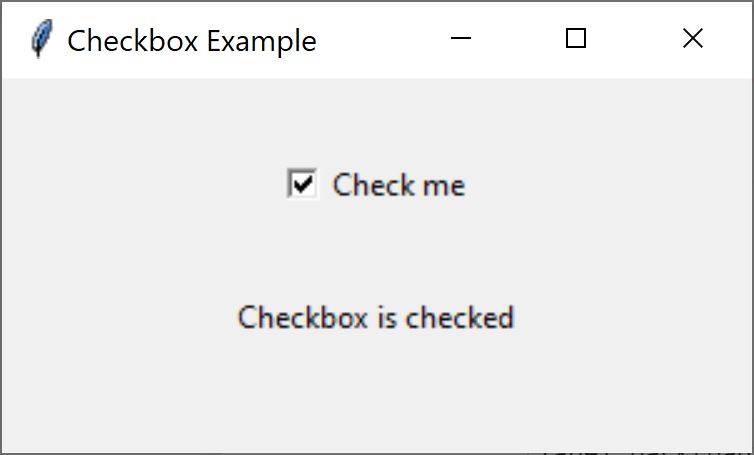
\includegraphics[width=0.6\textwidth]{images/checkbox.JPG}
    \caption{Tkinter}
    \label{fig:checkbox}
\end{figure}



\section{Network Programming}

\subsection{Terms and Networking Concepts}
Network programming refers to the practice of creating software that communicates over computer networks. Python provides several modules and libraries that facilitate network communication, making it relatively easy to develop networked applications.

\begin{itemize}
    \item \textbf{REST (Representational State Transfer)}\\
    REST is a style of software architecture for distributed systems, commonly used in networked applications like web services. It utilizes standard HTTP methods (GET, POST, PUT, DELETE) to manipulate resources, typically represented in formats such as JSON or XML. RESTful services follow principles such as statelessness, uniform interface, and resource-based interactions, making them scalable, flexible, and easily understandable.
    
    \item \textbf{Network Sockets}\\
    Network sockets are endpoints for communication between devices over a network. Sockets are used to establish connections and exchange data between a client and a server. They allow bidirectional data flow, enabling applications to send and receive data across networks using protocols such as TCP or UDP. Sockets provide an abstraction for handling network communication, allowing developers to create networked applications efficiently.
    
    \item \textbf{Protocols}\\
    Protocols are rules or standards that define how data is transmitted and received between devices on a network. They specify formats for data packets, error handling procedures, and other aspects of communication. Examples of network protocols include TCP/IP (Transmission Control Protocol/Internet Protocol), HTTP (Hypertext Transfer Protocol), and SMTP (Simple Mail Transfer Protocol).
    
    \item \textbf{Domains}\\
    Domains refer to the hierarchical naming system used to identify resources on the internet. They are part of the Domain Name System (DNS) and are used to assign memorable names to numerical IP addresses. For example, "google.com" is a domain name.
    
    \item \textbf{Addresses}\\
    Addresses are identifiers used to locate resources on a network, such as computers, servers, or other devices. In the context of the internet, addresses typically refer to IP addresses (Internet Protocol addresses), which are numerical labels assigned to each device connected to a computer network. For example, an IP address might be \texttt{192.0.2.1}.
    
    \item \textbf{Ports}\\
    Ports are virtual endpoints used by communication protocols to identify specific processes or services on a networked device. They allow multiple services or applications to operate concurrently on a single device. Ports are identified by numbers, and each service typically uses a specific port number. For example, web servers commonly use port 80 for HTTP and port 443 for HTTPS.
    
    \item \textbf{Services}\\
    Services refer to the software applications or processes running on a networked device that provide specific functions or features. These functions can include serving web pages, sending emails, transferring files, and more. Each service typically operates using one or more network protocols and may use specific ports for communication. Examples of services include web servers (e.g., Apache, Nginx), email servers (e.g., Microsoft Exchange, Postfix), and file transfer protocols (e.g., FTP, SFTP).
\end{itemize}

\newpage 
%\subsection{Network communication}

\subsubsection{Connection-oriented vs. Connectionless}
Network communication refers to the exchange of data between devices like computers, servers, routers, etc. over a network. This communication enables devices to share information, resources, and services. In networking, communication methods play a crucial role in determining how data is transmitted between devices. Two fundamental approaches are connection-oriented and connectionless communication. Connection-oriented communication establishes a dedicated link between sender and receiver for reliable data transfer, as seen in TCP. Conversely, connectionless communication, exemplified by UDP, sends independent packets without a prior connection, prioritizing speed over reliability.

\begin{itemize}
    \item \textbf{Connection-Oriented Communication:} In connection-oriented communication, a dedicated connection is established between the sender and receiver before any data transfer occurs. This connection remains active throughout the entire communication session. Protocols like TCP (Transmission Control Protocol) provide connection-oriented communication, ensuring reliable and ordered delivery of data.
    
    \item \textbf{Connectionless Communication:} In contrast, connectionless communication does not require a pre-established connection between the sender and receiver. Each data packet is sent independently and may take a different route to reach its destination. Protocols like UDP (User Datagram Protocol) operate in a connectionless manner. While connectionless communication is faster and more efficient for certain types of data, it may result in lost or out-of-order packets.
\end{itemize}

\subsubsection{Protocols: TCP and UDP}
A protocol is a set of rules or guidelines that govern how data is transmitted and received between devices, systems, or components in a networked environment. These rules define the format, timing, sequencing, and error handling of data transmission, ensuring that communication occurs in an organized, reliable, and efficient manner.\\

\begin{itemize}
    \item \textbf{Transmission Control Protocol (TCP)}
    \begin{itemize}
        \item Connection-oriented protocol
        \item Provides reliable, ordered, and error-checked delivery of data
        \item Uses acknowledgments and retransmissions for reliability
        \item Slower than UDP due to overhead of connection setup and error checking
        \item Suitable for applications requiring guaranteed delivery and data integrity, such as web browsing, email, and file transfer
    \end{itemize}

    \item \textbf{User Datagram Protocol (UDP)}
    \begin{itemize}
        \item Connectionless protocol
        \item Provides fast, but unreliable, delivery of data
        \item No guarantees on delivery, ordering, or duplicate protection
        \item Minimal overhead, making it faster than TCP
        \item Suitable for real-time applications, such as streaming media, online gaming, and VoIP, where speed is prioritized over reliability
    \end{itemize}
\end{itemize}

\newpage
\subsubsection{Clients and Servers}
In computer networking, clients and servers play integral roles in facilitating communication and accessing resources over a network. Clients, such as devices, programs, or processes, initiate requests for services or resources from servers.

\begin{itemize}
    \item \textbf{Clients:} Devices, programs, or processes that request services or resources from other devices or programs, known as servers. In a client-server model, clients initiate communication by sending requests to servers. These requests can vary widely depending on the type of service being requested. For example, a web browser acts as a client when it requests web pages from a web server, while an email client requests emails from an email server. Clients typically do not provide services directly to other devices or clients; instead, they rely on servers to fulfill their requests.
    
    \item \textbf{Servers:} Devices, programs, or processes that provide services, resources, or data to clients over a network. They listen for incoming requests from clients and respond by providing the requested services or resources. Servers can offer a wide range of services, including web hosting, email hosting, file storage, and database management. In a client-server model, servers are responsible for handling incoming requests from clients and delivering the appropriate responses. Unlike clients, servers do not typically initiate communication; instead, they wait for incoming requests from clients and respond accordingly.
\end{itemize}

The requests can vary depending on the service required, such as web pages or emails. Servers, on the other hand, respond to client requests by providing the requested services or resources. They listen for incoming requests and deliver appropriate responses, offering services like web hosting, email hosting, and file storage. Together, clients and servers form the foundation of the client-server model, enabling efficient communication and resource sharing across networks.\\

\begin{figure}[htbp]
    \centering
    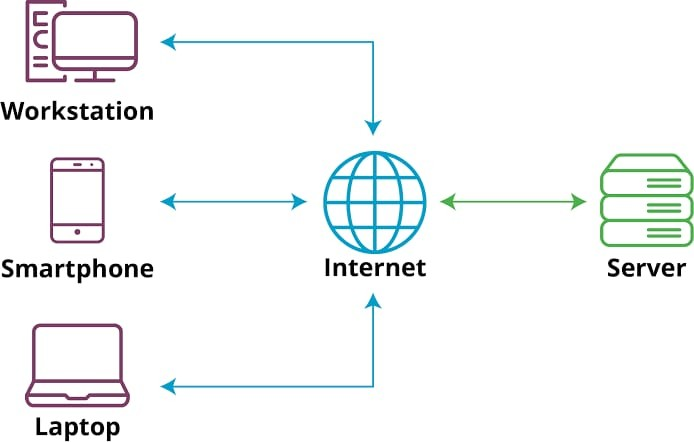
\includegraphics[width=0.7\textwidth]{images/client-server.jpg}
    \caption{Client server communication}
    \label{fig:example-np-2}
\end{figure}

\newpage
\subsection{Socket Programming}
Socket programming is a key aspect of network programming that enables communication between processes across a network. It forms the foundation for building various networked applications, allowing computers to exchange data over the internet or within a local network. In socket programming, a socket represents an endpoint for communication between two machines. A socket is an endpoint for communication between two machines. It consists of an IP address and a port number.
\begin{itemize}
    \item \textbf{IP Address:} An IP (Internet Protocol) address uniquely identifies a device on a network. In socket programming, IP addresses are used to establish connections between machines. An IP address is typically represented as a \textbf{32-bit number}, which is divided into four octets (each containing 8 bits) separated by periods. 
    \item \textbf{Port Number:} Port numbers are used to identify specific processes or services running on a machine. They facilitate multiplexing, allowing multiple applications to use the network simultaneously.
\end{itemize}

\begin{figure}[h!]
    \centering
    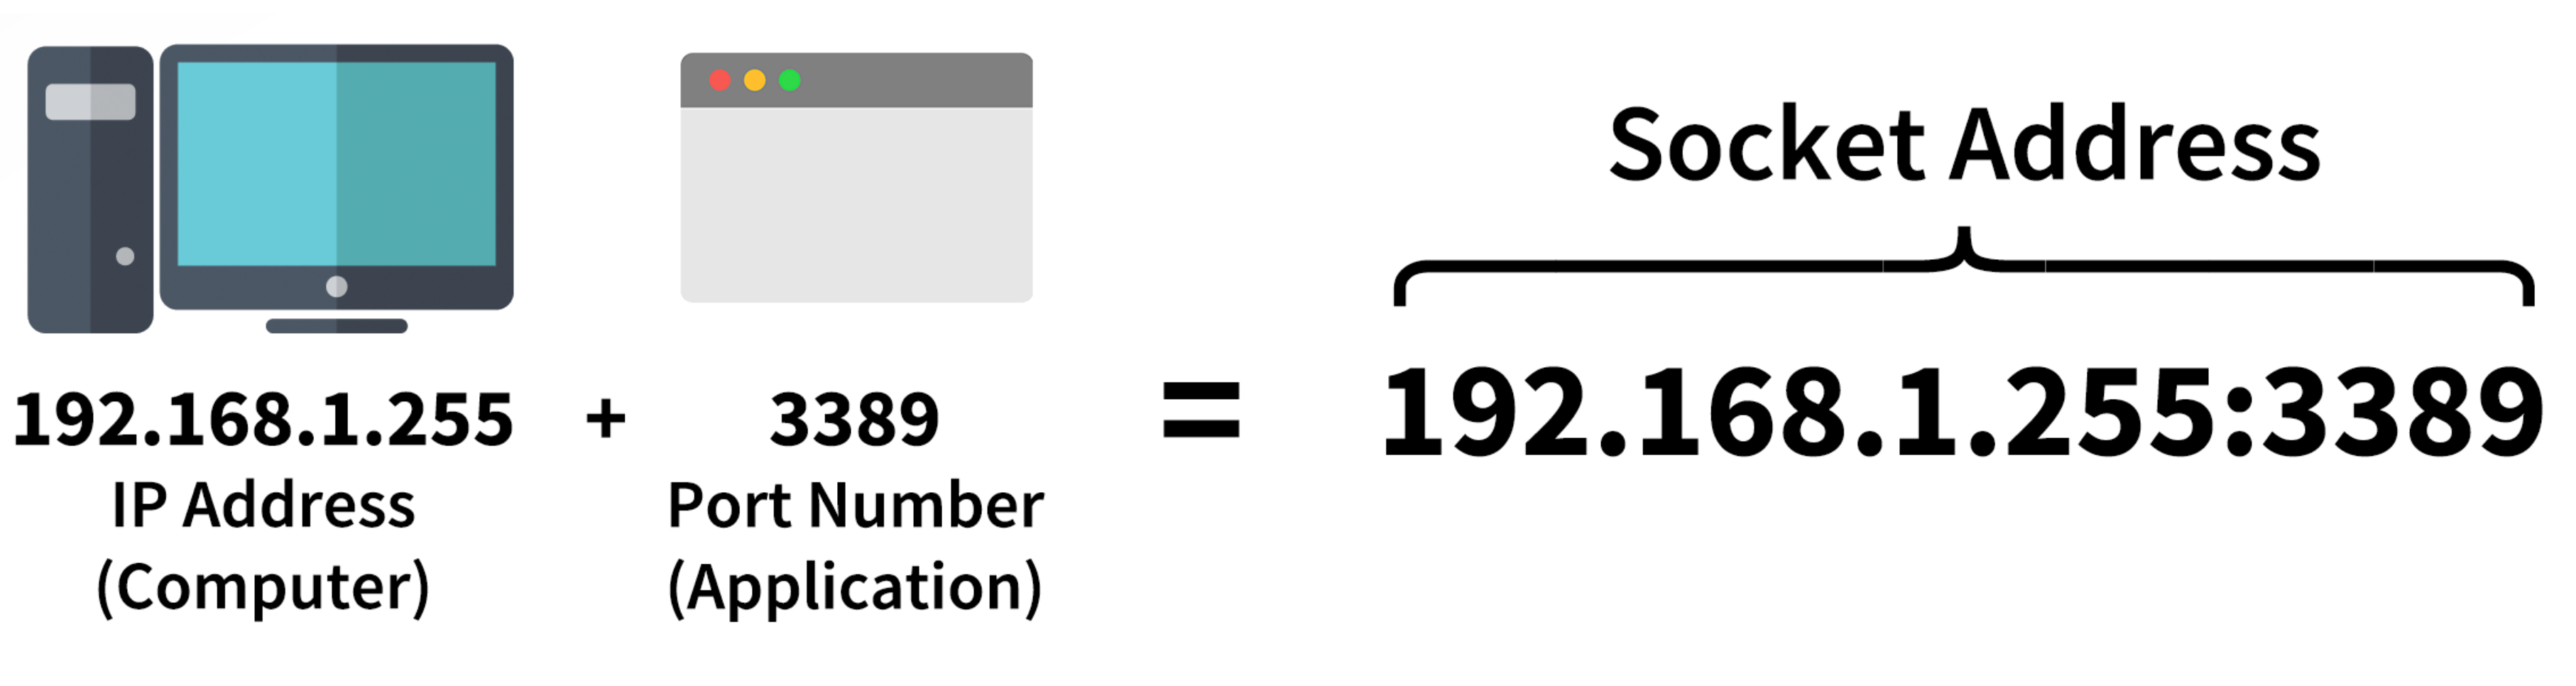
\includegraphics[width=0.6\textwidth]{images/socket_address.png}
    \caption{Socket address}
    \label{fig:example-np-1}
\end{figure}

\subsubsection{Types of Sockets}
\begin{itemize}[leftmargin=*]
    \item \textbf{Stream Sockets (TCP):} Stream sockets provide a reliable, connection-oriented communication channel. They ensure that data is delivered in the correct order without loss or duplication. TCP (Transmission Control Protocol) is commonly used for stream socket communication.
    \item \textbf{Datagram Sockets (UDP):} Datagram sockets provide an unreliable, connectionless communication channel. They allow for fast, low-overhead communication but do not guarantee delivery or order of messages. UDP (User Datagram Protocol) is commonly used for datagram socket communication.
\end{itemize}

\begin{codebox}
\begin{minted}{python}
import socket

# Creating a TCP socket
tcp_socket = socket.socket(socket.AF_INET, socket.SOCK_STREAM)

# Creating a UDP socket
udp_socket = socket.socket(socket.AF_INET, socket.SOCK_DGRAM)
\end{minted}
\end{codebox}

By specifying \texttt{socket.SOCK\_STREAM} for TCP and \texttt{socket.SOCK\_DGRAM} for UDP, the respective socket types are indicated to the \texttt{socket.socket()} function, allowing the creation of TCP or UDP sockets accordingly.

\newpage
\subsubsection{How Sockets Work}
\textbf{server.py}
\begin{codebox}
\begin{minted}{python}
import socket
import threading

SERVER = socket.gethostbyname(socket.gethostname()) # IP address of the server
PORT = 5050  # Port to listen on
ADDR = (SERVER, PORT)  # Address to bind the server
HEADER_SIZE = 64  # Size of the header containing message length
FORMAT = 'utf-8'  # Format to encode/decode messages
DISCONNECT_MSG = "!DISCONNECT"  # Message to disconnect a client

# Create a new socket
server = socket.socket(socket.AF_INET, socket.SOCK_STREAM)
server.bind(ADDR)

# Function to handle client connections
def handle_client(conn, addr):
    print(f"[NEW CONNECTION] {addr} connected")
    connected = True
    while connected:
        # Receive the header containing the message length
        header = conn.recv(HEADER_SIZE).decode(FORMAT)
        if header:
            msg_length = int(header)
            msg = conn.recv(msg_length).decode(FORMAT)
            if msg == DISCONNECT_MSG:
                connected = False
            print(f"[{addr}] {msg}")
            # Send acknowledgment to the client
            conn.send("[MESSAGE RECEIVED]".encode(FORMAT))
    conn.close()

# Function to start the server
def start():
    print(f"[LISTENING] server is listening on {SERVER}")
    server.listen()
    while True:
        # Wait for a new connection and store IP address and port
        conn, addr = server.accept()
        # Create a new thread to handle the client
        thread = threading.Thread(target=handle_client, args=(conn, addr))
        thread.start()
        print(f"[ACTIVE CONNECTIONS] {threading.active_count() - 1}")

if __name__ == "__main__":
    print("[STARTING] server is starting...")
    start()  # Start the server
\end{minted}
\end{codebox}

\newpage
\textbf{client.py}

\begin{codebox}
\begin{minted}{python}
import socket

# Get the IP address of the server dynamically
SERVER = socket.gethostbyname(socket.gethostname())
# Alternatively, specify IP address manually from ipconfig (IPv4 Address)
# SERVER = "192.168.12.30"
PORT = 5050  # Port on which the server is listening
ADDR = (SERVER, PORT)  # Address of the server
HEADER_SIZE = 64  # Size of the header containing message length
FORMAT = 'utf-8'  # Format to encode/decode messages
DISCONNECT_MSG = "!DISCONNECT"  # Message to disconnect from the server

# Create a new socket for the client
client = socket.socket(socket.AF_INET, socket.SOCK_STREAM)
client.connect(ADDR)

def send(message):
    # Encode the string message into bytes object
    message_encoded = message.encode(FORMAT)
    # Calculate the length of the encoded message
    message_length = str(len(message_encoded)).encode(FORMAT)
    # Pad the message length to ensure it matches HEADER_SIZE
    message_length += b' ' * (HEADER_SIZE - len(message_length))
    # Send the padded message length and the encoded message to the server
    client.send(message_length)
    client.send(message_encoded)

    # Receive messages from the server and print them
    print(client.recv(2048).decode(FORMAT))

# Send an initial message to the server
send("Hello, server!")

while True:
    # Continuously prompt the user for input
    msg = input("")

    if msg == "EXIT":
        # Send DISCONNECT_MSG to inform the server and break the loop
        send(DISCONNECT_MSG)
        break

    if msg:
        # If the user input is not empty, send it to the server
        send(msg)
\end{minted}
\end{codebox}

\newpage
\subsubsection{Connecting Sockets to HTTP Servers}
\begin{codebox}
\begin{minted}{python}
import socket

def send_http_request(host, port, request):
    # Create a socket object
    with socket.socket(socket.AF_INET, socket.SOCK_STREAM) as s:
        try:
            # Connect to the server
            s.connect((host, port))
            
            # Send the HTTP request
            s.sendall(request.encode())
            
            # Receive the response
            response = s.recv(4096)
            
            # Return the response
            return response.decode()
        
        except socket.error as e:
            print(f"Socket error: {e}")
        
        except Exception as e:
            print(f"An unexpected error occurred: {e}")
        
        finally:
            # Close the connection
            s.close()

# Example usage
if __name__ == "__main__":
    HOST = 'example.com'
    PORT = 80
    REQUEST = 'GET / HTTP/1.1\r\nHost: example.com\r\n\r\n'
    res = send_http_request(HOST, PORT, REQUEST)
    print(res)
\end{minted}
\end{codebox}

\begin{codebox}
\begin{minted}{python}
REQUEST = "GET / HTTP/1.1\r\nHost: www.example.com\r\n\r\n"
\end{minted}
\end{codebox}

This line is a string representing an HTTP request. It follows the HTTP protocol format:

\begin{itemize}
    \item \textbf{GET}: It's the HTTP method used to request data from a specified resource.
    \item \textbf{/}: It's the path of the resource being requested, in this case, it's the root path.
    \item \textbf{HTTP/1.1}: It specifies the version of the HTTP protocol being used.
    \item \textbf{\textbackslash r\textbackslash n}: It's a carriage return and line feed, used as a line break in HTTP requests.
    \item \textbf{Host: example.com}: It's a header specifying the domain name of the server.
    \item \textbf{\textbackslash r\textbackslash n}: Another line break.
    \item \textbf{\textbackslash r\textbackslash n}: An empty line indicating the end of the HTTP request headers.
\end{itemize}

\newpage
\subsubsection{Exceptions}
When working with Python sockets, which are used for network communication, there are several common exceptions. Handling these exceptions appropriately in your code ensures robustness and graceful error recovery during network communication.

\begin{itemize}
    \item \textbf{socket.error} or \textbf{socket.timeout}: These exceptions are the most general ones when working with sockets. They can occur for various reasons such as connection issues, timeouts, or other low-level socket errors.
    
    \item \textbf{ConnectionRefusedError}: This exception occurs when attempting to connect to a remote server that actively refuses the connection. It could indicate that the server is not running or is not accepting connections on the specified port.
    
    \item \textbf{ConnectionResetError}: This exception occurs when the connection is unexpectedly closed by the peer. It might happen due to network issues or if the peer terminates the connection unexpectedly.
    
    \item \textbf{BrokenPipeError}: This exception occurs when writing to a socket that has been closed at the other end. It typically happens when the connection is broken before all data has been sent or received.
    
    \item \textbf{TimeoutError}: This exception occurs when a socket operation times out. It can happen when attempting to establish a connection or during data transmission if there's no response within the specified timeout period.
    
    \item \textbf{OSError}: This is a general exception for various operating system-related errors. It can include errors related to file descriptors, permissions, or other low-level issues that might affect socket operations.
    
    \item \textbf{socket.gaierror}: This exception occurs when the address resolution fails. It could happen if the hostname cannot be resolved or if there's an issue with the network configuration.
    
    \item \textbf{socket.herror}: This exception occurs when a DNS-related error happens. It might occur when the DNS server is unreachable or if there's an issue with the hostname.
    
    \item \textbf{BlockingIOError}: This exception occurs when an operation would block if the \texttt{socket} is in non-blocking mode. It usually happens during non-blocking socket operations.
    
    \item \textbf{PermissionError}: This exception occurs when there's a permission-related issue, such as trying to bind to a privileged port without sufficient permissions.
\end{itemize}


\newpage
\subsection{REST Clients}
A REST (Representational State Transfer) client is a program or module that sends HTTP requests to a RESTful web service or API to interact with resources on the server. REST is an architectural style for designing networked applications, commonly used in web services development.

There are several libraries and frameworks available for creating REST clients. One popular choice is the \texttt{requests} library, which provides a simple and elegant way to send HTTP requests and handle responses.

\subsubsection{The \texttt{requests} Module}
The \texttt{requests} module simplifies the process of working with HTTP requests and responses, making it an essential tool for web scraping, web development, and interacting with web APIs.

\begin{codebox}
\begin{minted}{python}
import requests

# Making a GET request to the XKCD website
r = requests.get('https://xkcd.com/353/')

# Printing the available attributes and methods of the response object 'r'
#print(dir(r))

# Printing the help documentation for the response object 'r'
#print(help(r))

# Making a GET request to download the image from the XKCD website
img = requests.get('https://imgs.xkcd.com/comics/python.png')

# Printing the content of the image (binary data)
print(img.content)

# Printing the status code of the image request
print(img.status_code)

# If the response from the XKCD website is successful
if r.ok:
    # If response is ok, open a file named 'comic.png' in binary write mode
    with open('comic.png', 'wb') as f:
        # Write the binary content of the image to the file
        f.write(img.content)
\end{minted}
\end{codebox}

\newpage
\subsubsection{CRUD Operations}
CRUD is an acronym that stands for Create, Read, Update, and Delete. It represents the four basic operations that can be performed on data stored in a database or managed by an application:

\begin{itemize}
    \item \textbf{Create}: This operation involves adding new data or records to the database. In a database context, it typically means inserting a new row into a table. In an application context, it could involve creating new objects or entities.
    
    \item \textbf{Read}: This operation involves retrieving existing data or records from the database. In a database context, it typically means querying the database to retrieve specific data based on certain criteria. In an application context, it could involve fetching and displaying data to the user.
    
    \item \textbf{Update}: This operation involves modifying existing data or records in the database. In a database context, it typically means updating the values of one or more columns in a specific row. In an application context, it could involve allowing users to edit and update information.
    
    \item \textbf{Delete}: This operation involves removing existing data or records from the database. In a database context, it typically means deleting a row from a table. In an application context, it could involve allowing users to delete objects or entities.
\end{itemize}

CRUD operations form the foundation of many applications and are commonly used in various software systems, including web applications, mobile apps, and desktop applications. These operations allow users to interact with and manage data effectively, enabling applications to create, retrieve, update, and delete information as needed.

\subsubsection{HTTP Methods: GET, POST, PUT, DELETE}

HTTP (Hypertext Transfer Protocol) methods define the actions that a client (such as a web browser) can perform on a server. Each HTTP method is associated with a specific type of action that the client wants to perform on a resource identified by a URL.

\begin{itemize}
    \item \textbf{GET}: Used to retrieve data from a server, such as fetching a web page or an image.
    
    \item \textbf{POST}: Used for submitting data, uploading files, or making changes to a server's state.
    
    \item \textbf{PUT}: Used to update existing resources with new data.
    
    \item \textbf{DELETE}: Used to delete resources from a server, such as deleting a user account or a file.
\end{itemize}

\newpage
\begin{codebox}
\begin{minted}{python}
import requests

# Target URL for HTTP requests: https://httpbin.org/

# GET request with parameters passed directly in the URL
# r = requests.get('https://httpbin.org/get?page=2&count=25') # errorprone

# GET request with params
params = {'page':2, 'count': 25}
r = requests.get('https://httpbin.org/get', params=params)
print(r.url)
print(r.text)

# POST request with form data
form_data = {'username': 'corey', 'password': 'testing'}
r = requests.post('https://httpbin.org/post', data=form_data)
print(r.text)
r_dict = r.json()
print(r_dict['form'])

# GET request with Basic Authentication
auth = ('corey', 'testing')
r = requests.get('https://httpbin.org/basic-auth/corey/testing', auth=auth)
print(r)
print(r.text)

# Example of setting a timeout for a request
r = requests.get('https://httpbin.org/delay/1', timeout=2)
print(r)

# Example causing a timeout
r = requests.get('https://httpbin.org/delay/5', timeout=3)
print(r)
\end{minted}
\end{codebox}

\newpage
\subsubsection{Response Status Codes}
Response status codes are standardized three-digit integers that HTTP servers use to communicate the outcome of a client's request. They provide information about whether a request was successful, encountered an error, or requires further action. The status code is accompanied by a short, human-readable phrase that provides additional context. HTTP status codes are grouped into five categories, each represented by the first digit of the status code.

\begin{itemize}
    \item \textbf{1xx - Informational:}
    \begin{itemize}
        \item Request has been received and understood, and that further action is required by the client.
    \end{itemize}
    
    \item \textbf{2xx - Success:}
    \begin{itemize}
        \item \textbf{200 OK:} The request was successful.
        \item \textbf{201 Created:} The request has been fulfilled, and a new resource has been created.
        \item \textbf{204 No Content:} Request has been successfully processed by the server, but it is not returning any content.
    \end{itemize}
    
    \item \textbf{3xx - Redirection:}
    \begin{itemize}
        \item Further action is needed by the client to fulfill the request. They typically indicate that the client should take additional steps to complete the request.
    \end{itemize}
    
    \item \textbf{4xx - Client Error:}
    \begin{itemize}
        \item \textbf{400 Bad Request:} Server cannot process the request due to a client error, like invalid syntax.
        \item \textbf{401 Unauthorized:} Request requires authentication, but the client has not provided valid credentials.
        \item \textbf{404 Not Found:} Server cannot find the requested resource.
    \end{itemize}
    
    \item \textbf{5xx - Server Error:}
    \begin{itemize}
        \item \textbf{500 Internal Server Error:} Server encountered an unexpected condition that prevented it from fulfilling the request.
    \end{itemize}
\end{itemize}




Response status codes are essential for understanding the outcome of HTTP requests and diagnosing issues with web applications and APIs. By interpreting these status codes, clients can respond appropriately to the Server's response and handle errors or redirections effectively.

\newpage
\subsubsection{Analyzing the Server's Response}
Analyzing a server's response with the \texttt{requests} library involves examining various attributes of the response object returned by the requests module after making an HTTP request. Here's a basic overview of how to analyze a server's response using requests:

\begin{codebox}
\begin{minted}{python}
import requests

# Send a GET request
response = requests.get('https://api.example.com/data')

# Print the status code
print('Status Code:', response.status_code)

# Print the response headers
print('Headers:', response.headers)

# Print the response content as text
print('Response Text:', response.text)

# Print the URL of the response
print('URL:', response.url)

# Print any cookies sent by the server
print('Cookies:', response.cookies)

# Convert response content to JSON (if applicable)
try:
    json_data = response.json()
    print('Response JSON:', json_data)
except ValueError:
    print('Response is not in JSON format')

# Print time elapsed between sending the request and receiving the response
print('Elapsed Time:', response.elapsed.total_seconds(), 'seconds')
\end{minted}
\end{codebox}

\section{File Processing and Communicating with a Program’s Environment}


\subsection{SQLite}
\subsubsection{SQL}
SQL (Structured Query Language) is a domain-specific language used in programming and managing relational databases. It provides a standardized way of interacting with databases for tasks such as querying data, modifying data, defining schema, and managing access control.

\begin{itemize}
    \item \textbf{SELECT}\\
    The SELECT statement is used to retrieve data from one or more database tables. It can retrieve all columns, specific columns, or rows based on specified conditions.
    \begin{codebox}
    \begin{minted}{sql}
    -- Select all columns from a table
    SELECT * FROM table_name;

    -- Select specific columns from a table
    SELECT column1, column2 FROM table_name;

    -- Select with conditions
    SELECT * FROM table_name WHERE condition;
    \end{minted}
    \end{codebox}

    \item \textbf{INSERT INTO}\\
    The INSERT INTO statement is used to add new records (rows) into a table.
    \begin{codebox}
    \begin{minted}{sql}
    -- Insert into all columns
    INSERT INTO table_name VALUES (value1, value2, ...);

    -- Insert into specific columns
    INSERT INTO table_name (col1, col2, ...) VALUES (val1, val2, ...);
    \end{minted}
    \end{codebox}

    \item \textbf{UPDATE}\\
    The UPDATE statement is used to modify existing records in a table.
    \begin{codebox}
    \begin{minted}{sql}
    -- Update values in a table
    UPDATE table_name SET col1 = val1, col2 = val2 WHERE condition;
    \end{minted}
    \end{codebox}

    \item \textbf{DELETE}\\
    The DELETE statement is used to remove records from a table.
    \begin{codebox}
    \begin{minted}{sql}
    -- Delete all records from a table
    DELETE FROM table_name;

    -- Delete specific records based on condition
    DELETE FROM table_name WHERE condition;
    \end{minted}
    \end{codebox}
\end{itemize}

\subsubsection{SQLite}
The sqlite module is a built-in library that allows developers to interact with SQLite databases. SQLite is a lightweight, serverless database engine that stores data in a single file, making it convenient for small to medium-scale applications.

\subsubsection{Create a database}
This Python script connects - or creates if necessary - to an SQLite database named \texttt{customer.db}, creates a table named \texttt{customers} with three columns \texttt{first\_name}, \texttt{last\_name} and \texttt{email}, inserts one row, and inserts multiple rows using parameterized queries. Finally, it commits changes and closes the connection.
\begin{codebox}
\begin{minted}{python}
import sqlite3

# Connect to database, creating it if it doesn't exist
conn = sqlite3.connect('customer.db')

# Create a cursor
c = conn.cursor()

# Create a table with 3 columns
c.execute("""CREATE TABLE customers (
    first_name TEXT,
    last_name TEXT,
    email TEXT
)""")

# Insert one row
c.execute("""INSERT INTO customers VALUES 
            ('John', 'Elder', 'john@codemy.com')""")

# Insert multiple rows
many_customers = [
                 ('Alice', 'Smith', 'alice@example.com'),
                 ('Bob', 'Johnson', 'bob@example.com'),
                 ('Emma', 'Davis', 'emma@example.com'),
            ]
c.executemany("INSERT INTO customers VALUES (?,?,?)", many_customers)
            
# Commit command
conn.commit()

# Close the connection
conn.close()
\end{minted}
\end{codebox}

\begin{itemize}
    \item \textbf{\texttt{c.execute()}:} Executes a single SQL statement. Takes a string containing the SQL statement as its argument.
    
    \item \textbf{\texttt{c.executemany()}:} Executes multiple SQL statements with varying parameter values. Takes two arguments: a string containing the SQL statement with placeholders for parameters, and a sequence (e.g., list, tuple, or iterable) containing the parameter values.
    
    \item \textbf{\texttt{conn.commit()}:} Commits the current transaction. This means that all the changes made in the transaction are permanently saved to the database.
    
    \item \textbf{\texttt{conn.close()}:} Closes the database connection. It's important to close the connection after you're done using it to free up resources and ensure proper cleanup.
\end{itemize}


\newpage
\subsubsection{Data Types}
SQLite supports the following data types:

\begin{itemize}
    \item \textbf{NULL}: Used to indicate a missing or unknown value.
    \item \textbf{INTEGER}: Used for storing integer values.
    \item \textbf{REAL}: Used for storing floating-point numbers. It stores approximate numeric values.
    \item \textbf{TEXT}: Used for storing text strings, such as character data. It can store strings of any length.
    \item \textbf{BLOB}: Used for storing binary data, such as images, audio, or other types of files, of any size.
\end{itemize}

\subsubsection{Query a Database}
This Python script connects to an SQLite database named 'customer.db', queries the 'customers' table, fetches all data, prints it, commits changes, and closes the connection.
\begin{codebox}
\begin{minted}{python}
import sqlite3

conn = sqlite3.connect('customer.db')
c = conn.cursor()

# Query the databse
c.execute("SELECT * FROM customers")

#c.fetchone()
#c.fetchmany(3)
rows = c.fetchall()

for row in rows:
    print(row)

conn.commit()
conn.close()
\end{minted}
\end{codebox}

\begin{itemize}
    \item \textbf{\texttt{c.fetchone()}:} Retrieves the next single row from the result set.
    \item \textbf{\texttt{c.fetchmany(n)}:} Retrieves the next set of rows, where \texttt{n} determines how many rows to fetch.
    \item \textbf{\texttt{c.fetchall()}:} Retrieves all remaining rows from the result set and returns them as a list of tuples.
\end{itemize}

\newpage
\subsubsection{Updating and Deleting Data}
This code connects to an SQLite database file named "customer.db", creates a cursor object, updates all occurrences of 'John' to 'Tom' in the 'first\_name' column, deletes rows where the first name is 'Alice' and the last name is 'Smith', commits the changes, and finally closes the connection to the database.

\begin{codebox}
\begin{minted}{python}
import sqlite3

conn = sqlite3.connect('customer.db')
c = conn.cursor()

# Update 'John' to 'Tom'
c.execute(
    "UPDATE customers SET first_name = 'Tom' WHERE first_name = 'John'"
)

# Delete the rows where first name is 'Alice' and last name is 'Smith'
c.execute("""DELETE FROM customers 
             WHERE first_name = 'Alice' 
             AND last_name = 'Smith'""")

conn.commit()
conn.close()
\end{minted}
\end{codebox}

\textbf{Note:} The command \texttt{sqlite.connect()} creates a database if it doesn't exist.

\subsubsection{Transaction Demarcation}
Transaction demarcation refers to the delineation or boundary that separates one transaction from another within a database management system (DBMS). A transaction in this context is a sequence of operations (such as inserts, updates, or deletes) that are treated as a single logical unit of work.

\newpage
\subsection{JSON Files}
JSON (JavaScript Object Notation) files are a popular data interchange format used to store and exchange data between different platforms and programming languages. They are human-readable and easy to parse, making them a common choice for configuration files, web APIs, and data exchange between client and server. JSON files consist of key-value pairs organized into objects and arrays. The official JSON specification, requires double quotes for string values.\\

Here's a basic example of a JSON file:
\begin{codebox}
\begin{minted}{json}
{
  "name": "John Doe",
  "age": 30,
  "city": "New York",
  "is_student": false,
  "hobbies": ["reading", "traveling", "photography"],
  "address": {
    "street": "123 Main St",
    "city": "Anytown",
    "zip": "12345"
  }
}
\end{minted}
\end{codebox}

\subsubsection{Serialization and Deserialization}
\begin{itemize}    
    \item \textbf{json.dump(data, file.json)}\\ This function is used to \textit{serialize} Python objects into a JSON formatted file. It takes two arguments: the Python object to be serialized and a file object to which the JSON data will be written.
    
    \item \textbf{json.load(data, file.json)}\\ This function is used to \textit{deserialize} a JSON file or string. It takes a file object or a string containing JSON data as input and returns a Python object (typically a dictionary or a list) representing the JSON data.
    
    \item \textbf{json.dumps(data)}\\ This function is used to \textit{serialize} Python objects into a JSON formatted string. It takes a Python object as input and returns a string containing the JSON data.
    
    \item \textbf{json.loads(data)}\\ This function is used to \textit{deserialize} a JSON string. It takes a string containing JSON data as input and returns a Python object representing the JSON data.
\end{itemize}

\begin{codebox}
\begin{minted}{python}
import json

# JSON-formatted string
json_string = '[4, 3, "5.5", true, null, "code", {"one": "uno"}]'

# Deserialize JSON string into Python data structures
data = json.loads(json_string)
print(data) # [4, 3, '5.5', True, None, 'code', {'one': 'uno'}]
\end{minted}
\end{codebox}

In this example, \texttt{json.loads()} parses the JSON data stored in the \texttt{json\_string} variable and returns the corresponding Python data structure, which is then stored in the variable \texttt{data}.

\newpage
\subsubsection{Conversion}

\begin{table}[htbp]
\centering
\begin{tabular}{|c|c|c|}
\hline
\textbf{Type} & \textbf{Python} & \textbf{JSON} \\
\hline
Strings & \texttt{"hello" / 'hello'} & \textit{"hello" - wrapped in double quotes} \\
\hline
Numbers & \texttt{123} & \textit{No conversion needed} \\
\hline
Boolean Values & \texttt{True} / \texttt{False} & \texttt{true} / \texttt{false} \\
\hline
Sequence Types & Lists \texttt{[1, 2, 3]} / Tuples \texttt{(1, 2, 3)} & JSON arrays, represented by square brackets \\
\hline
Dictionaries & \texttt{\{"key": "value"\}} &  JSON objects, represented by curly braces \\
\hline
None / null & \texttt{None} & \texttt{null} \\
\hline
\end{tabular}
\caption{Conversion of Python datatypes to JSON}
\label{tab:conversion}
\end{table}

\subsubsection{Working with the \texttt{json} Module}
\begin{codebox}
\begin{minted}{python}
import json 

# Write the contents to the JSON file 'fruits.json'
with open('fruits.json', 'w') as file:
    data = []
    banana = {'name': 'Banana', 'calories': 100}
    data.append(banana)
    json.dump(data, file)
\end{minted}
\end{codebox}

Initially, a dictionary named \texttt{banana} with the keys \texttt{name} and \texttt{calories} is created. The dictionary is then appended to the list \texttt{data}. Subsequently, the list \texttt{data} is converted into JSON format using \texttt{json.dump()} and saved in the file \texttt{'fruits.json'}. 
\begin{codebox}
\begin{minted}{python}
import json 

# Read the contents from the JSON file 'fruits.json'
with open('fruits.json', 'r') as file:
    data = json.load(file)
    print(data) # Output: [{'name': 'Banana', 'calories': 100}]
    print(data[0]['name']) # Output: Banana
\end{minted}
\end{codebox}
To read from this JSON file, \texttt{json.load()} is used. It deserializes the JSON data from \texttt{'fruits.json'} and returns a list with the \texttt{banana} dictionary representing the JSON object.


\newpage
\subsection{CSV Files}
\subsubsection{Creating and Reading CSV Files}
CSV (Comma-Separated Values) files are plain text files that store tabular data in a structured format. Each line in a CSV file typically represents a row of data, and within each line, individual values are separated by commas or other delimiters, such as semicolons or tabs. CSV files are widely used for storing and exchanging data between different systems because they are simple, lightweight, and easily readable by both humans and computers.

\begin{codebox}
\begin{minted}{python}
import csv

# Data to be written to the CSV file
data = [
    ['Name', 'Age', 'Major'],
    ['Alice', 25, 'Computer Science'],
    ['Bob', 30, 'Engineering'],
    ['Charlie', 28, 'Mathematics'],
    ['David', 35, 'Physics']
]

# Open the file in write mode
with open('students.csv', 'w', newline='') as csvfile:
    # Create a CSV writer object
    writer = csv.writer(csvfile, delimiter=',')
    
    # Write the data to the CSV file
    writer.writerows(data)

print("CSV file 'students.csv' has been created successfully.")
\end{minted}
\end{codebox}

\begin{codebox}
\begin{minted}{python}
import csv

with open('students.csv', newline='') as csvfile:
    reader = csv.DictReader(csvfile, delimiter=',')
    print(f"Fieldnames: {reader.fieldnames}\n")
    for row in reader:
        for field, value in row.items():
            print(f"{field}: {value}")
        print()  # Print an empty line between each student's data
\end{minted}
\end{codebox}

\subsubsection{Excel}
Excel files are binary files created by Microsoft Excel or other spreadsheet software. They store data in a tabular format similar to CSV files but offer more features, such as formatting options, formulas, charts, and multiple sheets within a single file.

CSV files and Excel files are related in the sense that you can import CSV files into Excel or export data from Excel to CSV format. This interchangeability makes CSV files a common format for exchanging data between different programs and platforms, including Excel. Excel provides built-in functionality to open and save CSV files, allowing users to work with CSV data directly in Excel or import/export data between Excel and other software applications that support CSV format.

\newpage
\subsubsection{Processing CSV Files}
The \texttt{reader}, \texttt{writer}, \texttt{DictReader}, and \texttt{DictWriter} are classes provided by the \texttt{csv} module for reading and writing CSV files.

\begin{itemize}
    \item \texttt{reader}\\
     This class is used for reading data from a CSV file. It provides a simple interface for iterating over the lines in the CSV file, where each line is represented as a list of fields.
     
\begin{codebox}
\begin{minted}{python}
import csv

with open('data.csv', 'r') as file:
    csv_reader = csv.reader(file)
    for row in csv_reader:
        print(row)
\end{minted}
\end{codebox}
     
    
    \item \texttt{writer}\\
     This class is used for writing data to a CSV file. It provides methods for writing rows of data to the CSV file.
\begin{codebox}
\begin{minted}{python}
import csv

with open('data.csv', 'w', newline='') as file:
    csv_writer = csv.writer(file)
    csv_writer.writerow(['Name', 'Age', 'Country'])
    csv_writer.writerow(['Alice', 30, 'USA'])
    csv_writer.writerow(['Bob', 25, 'Canada'])
\end{minted}
\end{codebox}
    
    \item \texttt{DictReader}\\
    This class is similar to \texttt{reader}, but it returns each row as a dictionary where the keys are the field names and the values are the corresponding values in the row. This is useful when the CSV file has a header row.
\begin{codebox}
\begin{minted}{python}
import csv

with open('data.csv', 'r') as file:
    csv_dict_reader = csv.DictReader(file)
    for row in csv_dict_reader:
        print(row['Name'], row['Age'], row['Country'])
\end{minted}
\end{codebox}
    
    \item \texttt{DictWriter}\\
     This class is similar to \texttt{writer}, but it accepts dictionaries as input for writing rows. Each dictionary represents a row where keys correspond to field names.
\begin{codebox}
\begin{minted}{python}
import csv

with open('data.csv', 'w', newline='') as file:
    fieldnames = ['Name', 'Age', 'Country']
    csv_dict_writer = csv.DictWriter(file, fieldnames=fieldnames)
    csv_dict_writer.writeheader()
    csv_dict_writer.writerow(
    {'Name': 'Alice', 'Age': 30, 'Country': 'USA'})
    csv_dict_writer.writerow(
    {'Name': 'Bob', 'Age': 25, 'Country': 'Canada'})
\end{minted}
\end{codebox}
\end{itemize}


\newpage
\subsection{HTML / XML Documents}
HTML (Hypertext Markup Language) and XML (eXtensible Markup Language) are both markup languages used for structuring and presenting information on the internet. While they have similarities, they serve different purposes and have different syntax.\\

\textbf{HTML}
\begin{itemize}[label=$\bullet$]
  \item Used for creating web pages and web applications.
  \item Focuses on defining the structure and presentation of content.
  \item Contains predefined tags for elements like headings, paragraphs, lists, links, etc.
  \item Supports hypertext links for navigation.
  \item Often used in conjunction with CSS for styling.
  \item Example:
  \texttt{<h1>Hello, World!</h1>}
\end{itemize}

\textbf{XML}
\begin{itemize}[label=$\bullet$]
  \item Used for storing and transporting data.
  \item Focuses on describing the structure and meaning of data.
  \item Allows users to define custom tags to represent data.
  \item Hierarchical structure with nested elements.
  \item Platform and language agnostic, suitable for data exchange between systems.
  \item Example:\\ 
  \texttt{<book><title>The Kite Runner</title><author>Khaled Hosseini</author></book>}
%\begin{minted}{xml}
%<book>
%	<title>The Great Gatsby</title>
%	<author>F. Scott Fitzgerald</author>
%</book>
%\end{minted}
\end{itemize}

\subsubsection{Beautiful soup}
Beautiful soup is a Python library used for web scraping, particularly for parsing and extracting data from HTML and XML documents. While it can be used in combination with other libraries to fetch data from servers, it is not the primary library for making HTTP requests.

\begin{codebox}
\begin{minted}{python}
import requests
from bs4 import BeautifulSoup

# URL of the website you want to scrape
url = 'https://docs.python.org/3/'

# Sending a GET request to the URL
response = requests.get(url)

# Parsing the HTML content using BeautifulSoup
soup = BeautifulSoup(response.text, 'html.parser')

# Extracting the title of the webpage
title = soup.title.string
print("Title of the webpage:", title)
\end{minted}
\end{codebox}

\subsubsection{Sample XML Document}
\begin{codebox}
\begin{minted}{xml}
<?xml version="1.0" encoding="UTF-8"?>
<library>
    <book id="1">
        <title>Animal Farm</title>
        <author>George Orwell</author>
        <genre>Dystopian Fiction</genre>
        <year>1945</year>
    </book>
    <book id="2">
        <title>7 Habits of Highly Effective People</title>
        <author>Stephen R. Covey</author>
        <genre>Self-help</genre>
        <year>1989</year>
    </book>
    <book id="3">
        <title>Rich Dad Poor Dad</title>
        <author>Robert T. Kiyosaki</author>
        <genre>Personal Finance</genre>
        <year>1997</year>
    </book>
</library>
\end{minted}
\end{codebox}

\subsubsection{Document Type Definition (DTD)}
DTD and XML are two related concepts often used together to define and structure data in a document. DTD is a way to formally describe the structure and content of XML documents. It defines the rules that an XML document must follow. DTD specifies the elements and attributes that are allowed within the document, as well as their relationships and content types.

\begin{codebox}
\begin{minted}{dtd}
<!DOCTYPE library [
  <!ELEMENT library (book+)>
  <!ELEMENT book (title, author, genre, year)>
  <!ELEMENT title (#PCDATA)>
  <!ELEMENT author (#PCDATA)>
  <!ELEMENT genre (#PCDATA)>
  <!ELEMENT year (#PCDATA)>
]>
\end{minted}
\end{codebox}

\newpage
\subsubsection{The XML Tree Structure}

XML can be visualized and understood as a tree structure. An XML tree structure is a hierarchical representation of XML data, where elements are organized in a parent-child relationship.

% Define custom color
\definecolor{xmlgreen}{RGB}{0,128,0}
\definecolor{xmlred}{RGB}{186,33,33}
\definecolor{xmlolive}{RGB}{105,120,33}

\begin{itemize}
    \item \textbf{Root Element}
    \begin{itemize}
        \item The topmost element in the XML document.
        \item Acts as the parent element of all other elements.
        \item There can be only one root element in an XML document.
        \item Example: \textcolor{xmlgreen}{\texttt{<library>}}
    \end{itemize}
    
    \item \textbf{Elements}
    \begin{itemize}
        \item Basic building blocks of an XML document.
        \item Represented by tags enclosed in angle brackets (\texttt{<} and \texttt{>}).
        \item Can contain other elements, text content, or attributes.
        \item Example: \textcolor{xmlgreen}{\texttt{<book>}}
    \end{itemize}
    
    \item \textbf{Parent-Child Relationships}
    \begin{itemize}
        \item Elements can contain other elements, creating a hierarchical structure.
        \item The containing element is referred to as the parent, and the contained elements are its children.
        \item Children are nested within their parent elements.
        \item Example:
        
        \textcolor{xmlgreen}{\texttt{<book>}}
        
        \quad \texttt{\textcolor{xmlgreen}{<title>}Animal Farm\textcolor{xmlgreen}{</title>}}
        
        \quad \texttt{\textcolor{xmlgreen}{<author>}George Orwell\textcolor{xmlgreen}{</author>}}
        
   \textcolor{xmlgreen}{\texttt{</book>}}
    \end{itemize}
    
    \item \textbf{Attributes:}
    \begin{itemize}
        \item Provide additional information about elements.
        \item Attributes are specified within the start tag of an element.
        \item Each attribute consists of a name and a value.
        \item Example: \texttt{\textcolor{xmlgreen}{<book} \textcolor{xmlolive}{id=}\textcolor{xmlred}{"123"}\textcolor{xmlgreen}{>}}
    \end{itemize}
    
    \item \textbf{Text Content}
    \begin{itemize}
        \item Elements can contain text content.
        \item Text content is the data encapsulated within an element.
        \item Text content is stored as a child node of the element in the XML tree.
        \item Example: \texttt{\textcolor{xmlgreen}{<title>}Animal Farm\textcolor{xmlgreen}{</title>}}
    \end{itemize}
    
    \item \textbf{Sibling Elements}
    \begin{itemize}
        \item Elements that share the same parent are called siblings.
        \item Sibling elements are positioned at the same level within the XML hierarchy.
        \item They have the same parent but different names or content.
    \end{itemize}
\end{itemize}

\newpage
\subsubsection{Parsing XML Files with \texttt{xml.etree.ElementTree}}
Parsing XML in Python can be done using various libraries, but one of the most commonly used libraries is the built-in \texttt{xml.etree.ElementTree}. The \texttt{xml.etree.ElementTree} library provides a simple and efficient API for working with XML documents.

\begin{itemize}
    \item \textbf{Parsing XML}\\
    It provides functions to parse XML documents into an ElementTree object, which represents the hierarchical structure of the XML document. This allows easy traversal and manipulation of XML elements.
    
    \item \textbf{Creating XML}\\
    It allows the creation of new XML documents by constructing Element objects and building up the XML tree structure.
    
    \item \textbf{Navigating XML}\\
    \texttt{ElementTree} provides methods like \texttt{find()}, \texttt{findall()}, and \texttt{iter()} to navigate through XML elements, search for specific elements, and iterate over elements efficiently.
    
    \item \textbf{Accessing Element Attributes and Text}\\
    It provides methods to access attributes and text content of XML elements, making it easy to extract data from XML documents.
    
    \item \textbf{Modifying XML}\\
    \texttt{ElementTree} allows modification of XML documents by adding, removing, or modifying elements and their attributes.
    
    \item \textbf{Serializing XML}\\
    It supports serialization of the XML tree back into a string representation or writing it directly to a file.
\end{itemize}

\newpage
\subsubsection{Searching Data with \texttt{find()} and \texttt{findall()}}
The \texttt{find()} and \texttt{findall()} methods are used for searching and retrieving elements from an XML tree structure. Both methods traverse the XML tree starting from the element on which they are called and search through its descendants. They allow for efficient navigation and retrieval of elements based on their tag names. These methods are commonly used when processing XML data to extract specific information or manipulate the XML structure.

\begin{codebox}
\begin{minted}{python}
import xml.etree.ElementTree as ET

# Sample XML data
xml_data = '''
<people>
    <person>
        <name>John Doe</name>
        <age>30</age>
        <city>New York</city>
    </person>
    <person>
        <name>Jane Smith</name>
        <age>25</age>
        <city>Los Angeles</city>
    </person>
</people>
'''

# Parse the XML data
people = ET.fromstring(xml_data)

# Iterate over each 'person' element
for person in people.findall('person'):
    name = person.find('name').text
    age = int(person.find('age').text)
    city = person.find('city').text
    print(f"Name: {name}, Age: {age}, City: {city}")
\end{minted}
\end{codebox}

In this example, \texttt{xml.etree.ElementTree} is used to parse the XML data. The \texttt{fromstring()} method is used to parse the XML string and return the root element. Then, \texttt{findall()} method is used to find all the 'person' elements within the root element, and for each 'person' element, \texttt{find()} method is used to find child elements like 'name', 'age', and 'city'. Finally, their text content is extracted using the \texttt{text} property.

\newpage
\subsubsection{XPath Expressions}
XPath (XML Path Language) expressions are used to navigate through elements and attributes in an XML document. XPath provides a way to select nodes in an XML document by using a path-like syntax, similar to filesystem paths. XPath expressions can be used to pinpoint specific elements or attributes within an XML document based on their structure, content, or relationship to other elements.

XPath expressions are widely used in XML processing technologies such as XSLT (Extensible Stylesheet Language Transformations), XQuery, and XML parsers like lxml in Python or XPath libraries in other programming languages.

\begin{codebox}
\begin{minted}{python}
from lxml import etree

# XML document string
xml_string = """
<universities>
  <university name="Harvard University">
    <location>Cambridge, MA</location>
    <rank>1</rank>
  </university>
  <university name="Stanford University">
    <location>Palo Alto, CA</location>
    <rank>2</rank>
  </university>
  <university name="Massachusetts Institute of Technology (MIT)">
    <location>Cambridge, MA</location>
    <rank>3</rank>
  </university>
</universities>
"""

# Parse the XML string
root = etree.fromstring(xml_string)

# XPath expression to find names of all universities in "Cambridge, MA"
xpath_expr = "/universities/university[location='Cambridge, MA']/@name"

# Apply the XPath expression
selected_universities = root.xpath(xpath_expr)

# Print the selected university names
for university in selected_universities:
    print(university)
\end{minted}
\end{codebox}

The XPath expression to select the names of all universities located in "Cambridge, MA" is:
\textbf{\texttt{/universities/university[location='Cambridge, MA']/@name}}.\\

The expression \textbf{\texttt{//university/@name}} selects the \texttt{name} attribute of all \texttt{<university>}-elements.

\begin{itemize}
    \item \texttt{//university} selects all \texttt{<university>} elements, regardless of their depth within the hierarchy. \texttt{//element} selects all elements at any level of the XML hierarchy.
    \item \texttt{/@name} selects the \texttt{name} attribute of each selected \textless university\textgreater element.
\end{itemize}





\newpage
\subsubsection{Building XML Documents using the \texttt{Element} Class and the \texttt{SubElement} Function}
Creating XML documents can be done using the \texttt{Element} class and the \texttt{SubElement} function provided by the \texttt{xml.etree.ElementTree} module.

\begin{itemize}
    \item \textbf{Element class}
    \begin{itemize}
        \item The \texttt{Element} class represents an XML element.
        \item It is used to create individual XML elements with specific tag names.
        \item Syntax: \texttt{element = Element(tag)}, where \texttt{tag} is the name of the XML element.
        \item Example: \texttt{person\_element = Element("person")}.
    \end{itemize}
    
    \item \textbf{SubElement function}
    \begin{itemize}
        \item The \texttt{SubElement} function is used to create child elements and add them to a parent element.
        \item It takes three parameters: the parent element, the tag name of the child element, and optional attributes for the child element.
        \item Syntax: \texttt{SubElement(parent, tag, attrib=\{\})}.
        \item Example: \texttt{name\_element = SubElement(person\_element, "name")}.
    \end{itemize}
\end{itemize}

\begin{codebox}
\begin{minted}{python}
import xml.etree.ElementTree as ET

# Create root element
people = ET.Element("people")

# Create first person element
person1 = ET.SubElement(people, "person", id="1")
person1.text = "John Doe"
ET.SubElement(person1, "age").text = "30"
ET.SubElement(person1, "city").text = "New York"

# Create second person element
person2 = ET.SubElement(people, "person", id="2")
person2.text = "Jane Smith"
ET.SubElement(person2, "age").text = "25"
ET.SubElement(person2, "city").text = "Los Angeles"

# Create ElementTree object
tree = ET.ElementTree(people)

# Write XML to file or print it
tree.write("people.xml", encoding="utf-8", xml_declaration=True)
\end{minted}
\end{codebox}

\newpage
\subsection{Logging}
Logging is a mechanism used to record events that occur during program execution. It allows developers to track the flow of their program, identify errors, and monitor its behavior.The documentation for logging in Python can be found \href{https://docs.python.org/3/library/logging.html}{here}.

\begin{itemize}
    \item \textbf{Importing the logging module}\\
     Logging functionality is provided by the logging module, so the first step is usually to import it using \texttt{import logging}.
    
    \item \textbf{Configuring logging}\\
     Before logging anything, you typically configure the logging system. This includes setting the logging level, specifying the logging format, and determining where log messages should be stored or displayed. The \texttt{basicConfig()} function is commonly used to configure logging settings.
    
    \item \textbf{Creating loggers}\\
    Loggers are objects used to log messages. Each module or component in your program can have its own logger. You create a logger using \texttt{logging.getLogger(name)}, where \texttt{name} is typically the name of the module or component.
    
    \item \textbf{Logging messages}\\
    After creating loggers, you can utilize various logging methods to record messages at different severity levels:
    \begin{itemize}
        \item \texttt{debug()}: Used for low-level system details or debugging information.
        \item \texttt{info()}: Provides general informational messages about the system's operation.
        \item \texttt{warning()}: Logs potential issues that do not necessarily disrupt the functionality
        \item \texttt{error()}: Logs error messages for significant issues that affect the functionality.
        \item \texttt{critical()}: Logs critical issues that require immediate attention.
    \end{itemize}
    \item \textbf{Logging levels:} CRITICAL - ERROR - WARNING - INFO - DEBUG - NOTSET
\end{itemize}

% https://docs.python.org/3/library/logging.html#logrecord-attributes

\subsubsection{Configuration}
The \texttt{basicConfig} enables quick setup of logging by specifying basic options like log format, output destination, and minimum logging level. LogRecord attributes can be found \href{https://docs.python.org/3/library/logging.html#logrecord-attributes}{here}.


\begin{codebox}
\begin{minted}{python}
import logging

# Configure logging
logging.basicConfig(level=logging.INFO, filename="log.log", filemode="w",
                    format="%(asctime)s - %(levelname)s - %(message)s")

# Log messages at different levels
logging.debug("debug")          # Displayed by default
logging.info("info")            # Displayed if level is set to INFO or lower
logging.warning("warning")      # Always displayed
logging.error("error")          # Always displayed
logging.critical("critical")    # Always displayed
\end{minted}
\end{codebox}

\newpage
\subsubsection{Logging Variables or Exceptions}
This demonstrates basic logging functionality using the logging module.
\begin{codebox}
\begin{minted}{python}
import logging

# Setting up basic configuration for logging
logging.basicConfig(level=logging.DEBUG, filename="log.log", filemode="w",
                    format="%(asctime)s - %(levelname)s - %(message)s")

# Logging a variable
var = 2
logging.debug(f"The value of var is {var}")

# Logging an exception
try:
    1 / 0
except ZeroDivisionError as e:
    logging.error("Encountered a ZeroDivisionError", exc_info=True)
    logging.exception("Encountered a ZeroDivisionError")
\end{minted}
\end{codebox}

\subsubsection{Creating a Custom Logger, Handler and Formatter}
This code sets up a custom logging configuration, which includes configuring a logger, defining a file handler to direct log messages to a separate file, specifying a custom log message format, and logging a test message to verify the setup.
\begin{codebox}
\begin{minted}{python}
import logging

# Configure the basic logging settings
logging.basicConfig(level=logging.DEBUG, filename="log.log", filemode="w",
                    format="%(asctime)s - %(levelname)s - %(message)s")

# Creates a new logger if it doesn't already exist
# Using __name__ as the logger name ensures uniqueness and context relevance
logger = logging.getLogger(__name__)

# Define a file handler for logging to a separate file
handler = logging.FileHandler('tutorial.log')

# Define a custom formatter for the file handler
formatter = logging.Formatter(
    '%(asctime)s -  %(name)s - %(levelname)s - %(message)s')
handler.setFormatter(formatter)

# Add handler to the logger
logger.addHandler(handler)

# Log an informational message
logger.info("Test the custom logger")
\end{minted}
\end{codebox}

\subsubsection{LogRecord Attributes}

The LogRecord has a number of attributes, most of which are derived from the parameters to the constructor. (Note that the names do not always correspond exactly between the LogRecord constructor parameters and the LogRecord attributes.) These attributes can be used to merge data from the record into the format string. The following table lists (in alphabetical order) the attribute names, their meanings, and the corresponding placeholder.

\begin{longtable}{|l|l|p{8cm}|}
\hline
\textbf{Attribute} & \textbf{Format} & \textbf{Description} \\
\hline
args & Not formatted directly & Tuple of arguments merged into msg to produce message or dictionary values used for the merge (when only one argument and it is a dictionary). \\
asctime & \%(asctime)s & Human-readable time when LogRecord was created (e.g., '2003-07-08 16:49:45,896' with millisecond portion after comma). \\
created & \%(created)f & Time when LogRecord was created (as returned by time.time()). \\
exc\_info & Not formatted directly & Exception tuple (à la sys.exc\_info) or None if no exception occurred. \\
filename & \%(filename)s & Filename portion of pathname. \\
funcName & \%(funcName)s & Name of function containing the logging call. \\
levelname & \%(levelname)s & Text logging level for the message ('DEBUG', 'INFO', 'WARNING', 'ERROR', 'CRITICAL'). \\
levelno & \%(levelno)s & Numeric logging level for the message (DEBUG, INFO, WARNING, ERROR, CRITICAL). \\
lineno & \%(lineno)d & Source line number where logging call was issued (if available). \\
message & \%(message)s & Logged message, computed as msg \% args. Set when Formatter.format() is invoked. \\
module & \%(module)s & Module (name portion of filename). \\
msecs & \%(msecs)d & Millisecond portion of time when LogRecord was created. \\
msg & Not formatted directly & Format string passed in original logging call, merged with args to produce message. \\
name & \%(name)s & Name of logger used to log the call. \\
pathname & \%(pathname)s & Full pathname of source file where logging call was issued (if available). \\
process & \%(process)d & Process ID (if available). \\
processName & \%(processName)s & Process name (if available). \\
relativeCreated & \%(relativeCreated)d & Time in milliseconds when LogRecord was created, relative to time the logging module was loaded. \\
stack\_info & Not formatted directly & Stack frame information (where available) from bottom of stack in current thread, up to and including stack frame of logging call which resulted in creation of this record. \\
thread & \%(thread)d & Thread ID (if available). \\
threadName & \%(threadName)s & Thread name (if available). \\
taskName & \%(taskName)s & asyncio.Task name (if available). \\
\hline
\end{longtable}
LogRecord attributes can be found \href{https://docs.python.org/3/library/logging.html#logrecord-attributes}{here}.

\newpage
\subsection{INI Files}
INI (initialization) files are simple text-based configuration files commonly used to store configuration settings for software applications. The name "INI" comes from the filename extension ".ini" often used for such files.\\

INI files consist of sections, each containing key-value pairs that represent configuration settings. The format is straightforward, typically resembling the following:

\begin{codebox}
\begin{minted}{ini}
[DEFAULT]
host = localhost # This is a comment.
 
[mariadb]
name = hello
user = user
password = password
 
[redis]
port = 6379
db = 0
\end{minted}
\end{codebox}


\begin{itemize}
    \item \textbf{Sections:} Sections are enclosed in square brackets ([]) and provide a way to group related configuration settings together. Sections help organize settings and prevent naming conflicts between keys.
    \item \textbf{Keys and Values:} Each key-value pair represents a configuration setting. The key is separated from the value by an equal sign (=). Keys are unique within a section and are used to identify specific configuration options, while values represent the corresponding settings.
\end{itemize}

\subsubsection{Interpolating Values in .ini Files}
Interpolating values in .ini files refers to the process of replacing placeholders or variables within the configuration file with actual values. This is commonly done to make configuration files more dynamic and reusable.

For example, consider an .ini file with the following content:
\begin{mdframed}[linewidth=1pt,linecolor=black,backgroundcolor=white]
\begin{minted}{text}
[Paths]
base_path = /home/user
data_path = %(base_path)s/data
log_path = %(base_path)s/logs
\end{minted}
\end{mdframed}

In this file, \texttt{\%()} syntax is used to define placeholders. When values are interpolated, the placeholders are replaced with the actual values they represent. For instance, if \texttt{base\_path} is \texttt{/home/user}, then after interpolation, \texttt{data\_path} will become \texttt{/home/user/data} and \textit{log\_path} will become \texttt{/home/user/logs}.

Interpolating values in .ini files allows for more flexible and reusable configuration management, as it enables referencing and reusing values defined elsewhere in the configuration file. This can be particularly useful for managing paths, URLs, and other repetitive configurations.

\newpage
\subsubsection{The \texttt{configparser}}

The \texttt{configparser} object is part of the standard library module \texttt{configparser}. It provides a way to work with configuration files in a consistent, easy-to-use manner. Configuration files are typically used to store settings and parameters for applications.

\begin{codebox}
\begin{minted}{python}
from configparser import ConfigParser

config = ConfigParser()

config["Server"] = {
    "hostname": "example.com",
    "port": "8080",
    "protocol": "http"
}

config["Database"] = {
    "db_name": "example_db",
    "db_user": "admin",
    "db_password": "strong_password"
}

with open("app_config.ini", "w") as f:
    config.write(f)
\end{minted}
\end{codebox}

This creates the following INI File:
\begin{mdframed}[linewidth=1pt,linecolor=black,backgroundcolor=white]
\begin{minted}{text}
[Server]
hostname = example.com
port = 8080
protocol = http

[Database]
db_name = example_db
db_user = admin
db_password = strong_password
\end{minted}
\end{mdframed}

\begin{codebox}
\begin{minted}{python}
from configparser import ConfigParser

config = ConfigParser()
config.read("app_config.ini")

# Extracting configuration from the sections
server_config = config["Server"]
database_config = config["Database"]

# Displaying configuration values
print("Server Configuration:")
print(f"Hostname: {server_config['hostname']}")
print(f"Port: {server_config['port']}")
print(f"Protocol: {server_config['protocol']}")
\end{minted}
\end{codebox}
\section{PCPP1 Certification}
\subsection{Exam Syllabus}
%
\includepdf[pages=-]{../pdf_pcpp1/pcpp1.pdf}

The exam syllabus can be accessed \href{https://pythoninstitute.org/assets/628def5091da2303121759.pdf}{here}.

\begin{table}[htbp]
    \centering
    \begin{tabular}{lll} % Define the columns with left-aligned, left-aligned, and right-aligned alignment
        \toprule
        \textbf{Section} & \textbf{Items} & \textbf{Max Score} \\
        \midrule
        Section 1: Advanced Object-Oriented Programming & 15 & 42 (35\%) \\
        Section 2: Coding Conventions, Best Practices, and Standarization  & 7 & 14 (12\%) \\
        Section 3: GUI Programming & 8 & 24 (20\%) \\
        Section 4: Network Programming & 8 & 22 (18\%) \\
        Section 5: File Processing and Communicating with a Program’s Environment & 7 & 18 (15\%) \\
        \bottomrule
    \end{tabular}
    \caption{Exam Syllabus}
    \label{tab:exam_sections}
\end{table}

%\newpage
%\begin{figure}[h!]
%    \centering
%    
\includegraphics[angle=90,width=1\textwidth]{cert/pcpp1.jpg}
%    %\caption{PCPP1}
%    \label{fig:pcpp1}
%\end{figure}

%\subsection{Exam Questions}

\subsubsection{Shallow Copy vs Deep Copy}
\begin{itemize}
    \item \textbf{copy.copy(original\_list)}: This method creates a shallow copy of \texttt{original\_list}. It means that the top-level elements of the list are copied, but the nested lists are still referenced. Therefore, modifying elements within the nested lists in the copied list will affect the original list as well.
    
    \item \textbf{copy.deepcopy(original\_list)}: This method creates a deep copy of \texttt{original\_list}. It recursively copies all nested lists and objects within \texttt{original\_list}, creating new objects in memory. Therefore, modifying elements within the nested lists in the copied list will not affect the original list.
\end{itemize}

\begin{codebox}
\begin{minted}{python}
# Original list containing strings and a nested list
title = ['Python', 'Course', [3, 10, 0]]

# Shallow copy of the original list
copied = title[:]

# Modify the nested list in the original list
copied[2][1] = 11
copied[0] = "React"

# Print the original list and the shallow copy
print(title)  # Output: ['Python', 'Course', [3, 11, 0]]
print(copied) # Output: ['React', 'Course', [3, 11, 0]]
\end{minted}
\end{codebox}

This operation is known as a \textbf{shallow copy} because it creates a new list object, but it does not create new copies of the elements within the list. If the elements are mutable objects (like lists or dictionaries), changes made to those elements in \texttt{copied} will also be reflected in the original list, and vice versa. However, if the elements are immutable (like integers or strings), they are effectively copied, and changes made to them in one list will not affect the other.

\subsubsection{Copying Comparison}
\begin{codebox}
\begin{minted}{python}
import copy
 
a = [[1, 2], [3, 4]]
 
b = copy.copy(a)
c = copy.deepcopy(a)
 
b[0][0] = 10
c[0][0] = 20

print(a)   # [[10, 2], [3, 4]]
print(b)   # [[10, 2], [3, 4]]
print(c)   # [[20, 2], [3, 4]]
\end{minted}
\end{codebox}

\subsubsection{Copying Performance}
Deep copy will have the worst performance among the provided copy operations. Deep copying, as performed by copy.deepcopy(), creates a new object and recursively copies all nested objects within it. In the case of a large and complex data structure, deep copying can be computationally expensive and time-consuming. It requires traversing the entire structure, creating new objects, and copying the values of all nested objects.

\subsubsection{Copies and id()}
\begin{codebox}
\begin{minted}{python}
title = 'Python Course'
var = title
 
print(f'title ID: {id(title)}') # title ID: 2081709060592
print(f'var ID: {id(var)}')     # var ID: 2081709060592
print(title == var)             # True
print(title is var)             # True
\end{minted}
\end{codebox}

\subsubsection{Deep copy of string}
In the following code example, \texttt{copy.deepcopy()} is used to create a deep copy of the \texttt{title} variable. A deep copy creates a new object and recursively copies the contents of the original object, so changes made to the copied object do not affect the original object, and vice versa.\\

\begin{codebox}
\begin{minted}{python}
import copy

title = 'Python Course'
var = copy.deepcopy(title)
 
print(f'title ID: {id(title)}') # title ID: 2081702974320
print(f'var ID: {id(var)}')     # var ID: 2081702974320
print(title == var)             # True
print(title is var)             # True
\end{minted}
\end{codebox}

However, in this specific case, since the \texttt{title} variable is a string, which is immutable in Python, the deep copy operation does not actually create a new object. Python optimizes memory usage for immutable objects, \textbf{so when a deep copy is made of an immutable object, Python will reuse the existing object rather than creating a new one}.

\subsubsection{Copies}
\begin{codebox}
\begin{minted}{python}
title = ['Python', 'Course', '3.10'] 
copy = title[:]
 
print(f'title ID: {id(title)}') # ...504
print(f'copy ID: {id(copy)}') # ...616
print(title == copy) # True
print(title is copy) # False

print(id(title[0])) # ...040
print(id(copy[0]))  # ...040
\end{minted}
\end{codebox}

\begin{itemize}
\item \texttt{copy = title[:]}: This line creates a shallow copy of the title list and assigns it to the variable copy. The [:] slice notation creates a copy of the entire list.
\item \texttt{print(f'title ID: {id(title)}')}: This line prints the ID of the title list.
\item \texttt{print(f'copy ID: {id(copy)}')}: This line prints the ID of the copy list.
\item \texttt{print(title == copy)}: This line compares the content of the title and var lists. It will return True if the lists have the same elements in the same order, and False otherwise.
\item \texttt{print(title is copy)}: This line checks if title and copy refer to the same object (same ID) in memory. It will return True if title and var are the same object, and False otherwise.
\end{itemize}

\subsubsection{What does the \texttt{id()} function?}
The id() function in Python returns a unique identifier for an object. It is an integer value that represents the "identity" of the object. This identity is guaranteed to be unique and constant for the object during its lifetime, meaning that it will not change as long as the object exists.

\subsubsection{What function determines the type of an object, including functions and classes?}
The \texttt{type()} function is used to determine the type of an object. It can be used with various types of objects, including functions and classes.

\begin{itemize}
    \item \textbf{Type of a Function:} When you use \texttt{type()} with a function, it returns the type of the function object, which is typically \texttt{<class 'function'>}.
    
    \item \textbf{Type of a Class:} When you use \texttt{type()} with a class, it returns the type of the class object, which is typically \texttt{<class 'type'>}.
\end{itemize}

\begin{codebox}
\begin{minted}{python}
def my_func():
    pass

class MyClass:
    pass

print(type(my_func)) # <class 'function'>
print(type(MyClass)) # <class 'type'>
\end{minted}
\end{codebox}

\subsubsection{Logging}
\textbf{In a Python application, you want to customize the format of the log messages. You decide to include the time of logging, the severity level of the message, the module where the event occurred, and the message itself. Which of the following formatting strings would be the most appropriate for this purpose?}\\

\texttt{\%(asctime)s - \%(levelname)s - \%(module)s - \%(message)s}\\

This format string includes the time (\%(asctime)s), the module where the event occurred (\%(module)s), the severity level of the message (\%(levelname)s), and the message itself (\%(message)s).\\

\subsubsection{Which of the following logs represents the default formatting of the root logger in the logging module?}

\texttt{CRITICAL:root:Message}.\\
In the logging module of Python, the default log message format consists of the following components:

\begin{itemize}
    \item \textbf{LEVEL:} Represents the severity level of the log message, such as DEBUG, INFO, WARNING, ERROR, or CRITICAL.
    \item \textbf{LOGGER\_NAME:} The name of the logger used to log the message. The root logger, which is the main logger in the logging hierarchy, is named "root" by default.
    \item \textbf{MESSAGE:} The actual content of the log message.
\end{itemize}

\subsubsection{Logging}
\textbf{The \texttt{logging.basicConfig} function is used to configure the logging module in Python. It allows you to specify the format of log messages using the \texttt{format} argument. The desired log format can be achieved by specifying the appropriate format string with the required attributes of the \texttt{LogRecord} object. What formatting should you apply to get the following?}\\

\texttt{2024-02-08 16:35:27,164 krako WARNING:Your log message}

\begin{codebox}
\begin{minted}{python}
import logging
 
FORMAT = '%(asctime)s %(user)s %(levelname)s:%(message)s'
logging.basicConfig(format=FORMAT)
\end{minted}
\end{codebox}

The \texttt{logging.basicConfig(format=FORMAT)} call sets the format of the root logger to the specified format. This ensures that all subsequent log messages logged through the root logger will use the specified format.
\begin{itemize}
    \item \texttt{\%asctime}: The timestamp of the log entry in the format "YYYY-MM-DD HH:MM:SS,sss".
    \item \texttt{\%user}: The user attribute of the \texttt{LogRecord} object. (Note: This attribute is not available by default, so you may need to add it yourself if it's not present in the \texttt{LogRecord}.)
    \item \texttt{\%levelname}: The log level of the message, e.g., "WARNING" in this case.
    \item \texttt{:} A separator between the log level and the log message.
    \item \texttt{\%message}: The actual log message.
\end{itemize}

\subsubsection{As a Python Developer, you need to work with logging events in your application. Which of the following snippet of code will return the root logger?}
\begin{codebox}
\begin{minted}{python}
import logging
 
logger = logging.getLogger()
\end{minted}
\end{codebox}
In the Python logging module, the \texttt{getLogger()} function is used to retrieve a logger object. By default, if no name is provided as an argument to \texttt{getLogger()}, it returns the root logger.

\newpage
\subsubsection{How can you access the docstring of a function?}

\begin{codebox}
\begin{minted}{python}
def my_function():
    """One-line description."""
    pass

print(my_function.__doc__) # One-line description.
\end{minted}
\end{codebox}

%%%%%%%%%%%%%%%%%%%%%%%%%%%% XML %%%%%%%%%%%%%%%%%%%%%%%%%%

\subsubsection{XML}
\begin{codebox}
\begin{minted}{python}
import xml.etree.ElementTree as ET

# XML string
xml_as_string = '''<?xml version="1.0"?>
<catalog>
   <book id="bk101">
      <author>Gambardella, Matthew</author>
      <title>XML Developer's Guide</title>
      <genre>Computer</genre>
   </book>
   <book id="bk102">
      <author>Ralls, Kim</author>
      <title>Midnight Rain</title>
      <genre>Fantasy</genre>
   </book>
</catalog>'''

# Parse the XML string
root = ET.fromstring(xml_as_string)

# Print tag names and attributes of each element
for child in root:
    print(f'{child.tag} -> {child.attrib}')

# Output
# book -> {'id': 'bk101'}
# book -> {'id': 'bk102'}
\end{minted}
\end{codebox}

\subsubsection{XML Root Element}

In Python's \texttt{xml.etree.ElementTree} module the method \texttt{getroot()} returns the root element of an ElementTree object. Therefore, to obtain the root element of the XML tree represented by the tree object in the provided code, you would use the \texttt{getroot()} method.

\begin{codebox}
\begin{minted}{python}
import xml.etree.ElementTree as ET
tree = ET.parse('products.xml')
root_element = tree.getroot()  # Retrieves the root element of the XML tree
\end{minted}
\end{codebox}

\newpage
\subsubsection{Parsing XML}
\begin{codebox}
\begin{minted}{python}
import xml.etree.ElementTree as ET

# Define the XML string
xml_as_string = """<?xml version="1.0"?>
<catalog>
   <book id="bk101">
      <author>Gambardella, Matthew</author>
      <title>XML Developer's Guide</title>
      <genre>Computer</genre>
      <price>44.95</price>
   </book>
   <book id="bk102">
      <author>Ralls, Kim</author>
      <title>Midnight Rain</title>
      <genre>Fantasy</genre>
      <price>5.95</price>
   </book>
</catalog>"""

# Parse the XML string
root = ET.fromstring(xml_as_string)
print(root[0])           # <Element 'book' at 0x000002C183BEF290>
print(root[0][0])        # <Element 'author' at 0x000002C183BEFC90>
print(root[0][0].text)   # Gambardella, Matthew
print(root[1][3].text)   # 5.95
\end{minted}
\end{codebox}

\subsubsection{XPath}
XPath is a query language for selecting nodes from an XML document. When using XPath, the \texttt{@name} syntax is used to select attributes with the specified name. Here's how it works:
\begin{codebox}
\begin{minted}{text}
<bookstore>
  <book name="Harry Potter">
    <author>J.K. Rowling</author>
    <price>20</price>
  </book>
  <book name="The Hobbit">
    <author>J.R.R. Tolkien</author>
    <price>25</price>
  </book>
</bookstore>
\end{minted}
\end{codebox}
If you want to select nodes based on the value of an attribute named "name", you would use the \texttt{[@name]} syntax in your XPath expression. This will select nodes that have a "name" attribute, regardless of its value. 
\begin{itemize}
\item If you want to select all \texttt{<book>} elements that have a "name" attribute, you would use the XPath expression: \textbf{\texttt{//book[@name]}}
\item To find all books named "The Hobbit" in the XML document, you can use the following XPath expression: \textbf{\texttt{//book[@name='The Hobbit']}}
\end{itemize}

\subsubsection{XPath indices}
\textbf{XPath indices start at 1, not 0.} When using XPath to navigate XML documents or select nodes, you start counting from 1 for the first node, 2 for the second node, and so on. This is consistent with many other programming languages and standards where indexing typically starts at 1 instead of 0.\\

\texttt{/store/book[2]/author}: This XPath expression correctly selects the author of the \textbf{second} book in the store.

\subsubsection{Document Type Definition (DTD)}
\textbf{Consider the following Document Type Definition (DTD) for an XML document:}
\begin{minted}{text}
<!DOCTYPE bookstore [
  <!ELEMENT bookstore (book*)>
  <!ELEMENT book (title, author, year, price)>
  <!ATTLIST book category CDATA #REQUIRED>
  <!ELEMENT title (#PCDATA)>
  <!ELEMENT author (#PCDATA)>
  <!ELEMENT year (#PCDATA)>
  <!ELEMENT price (#PCDATA)>
]>
\end{minted}

\begin{itemize}
\item \textbf{The "book" element must contain the child elements in the order of "title", "author", "year", and "price".} According to the DTD, the "book" element must contain the child elements in the specified order: "title", "author", "year", and "price".

\item \textbf{The "book" element must have an attribute called "category" of type CDATA.} The DTD specifies that the "book" element must have an attribute called "category" with a type of CDATA. The \texttt{\#REQUIRED} keyword indicates that the attribute is mandatory.

\item \textbf{\texttt{\#PCDATA}} stands for "Parsed Character Data." It is a keyword used to specify that an element can contain character data that will be parsed by the XML parser.\\

\item \textbf{\texttt{!ELEMENT}} is used to define the structure of elements (their names and content models), while \texttt{!ATTLIST} is used to define the attributes of elements (their names, datatypes, and properties).
\end{itemize}

\subsubsection{XML Attributes}
\begin{codebox}
\begin{minted}{xml}
<person id="123" gender="female">
    <name>Emma</name>
    <age>30</age>
</person>
\end{minted}
\end{codebox}

In this code example, \texttt{id} and \texttt{gender} are attributes of the \texttt{<person>} element.

\subsubsection{XML - Comments}
In XML (eXtensible Markup Language), comments are used to add explanatory or informative text that is not processed by the XML parser. An XML comment is a text surrounded by \texttt{<!-- and !-->}.

\newpage
\subsubsection{Write XML}
You can use the \texttt{xml.etree.ElementTree} module in Python to create the XML file. This code will create an XML file named "books.xml" with the specified structure and content.
\begin{codebox}
\begin{minted}{python}
import xml.etree.ElementTree as ET

# Create the root element
catalog = ET.Element("catalog")

# Create the first book element
book1 = ET.SubElement(catalog, "book", id="bk101")
book1.text = ""
ET.SubElement(book1, "author").text = "Gambardella, Matthew"
ET.SubElement(book1, "title").text = "XML Developer's Guide"
ET.SubElement(book1, "genre").text = "Computer"
ET.SubElement(book1, "price").text = "44.95"
ET.SubElement(book1, "publish_date").text = "2000-10-01"

# Create the second book element
book2 = ET.SubElement(catalog, "book", id="bk102")
book2.text = ""
ET.SubElement(book2, "author").text = "Ralls, Kim"
ET.SubElement(book2, "title").text = "Midnight Rain"
ET.SubElement(book2, "genre").text = "Fantasy"
ET.SubElement(book2, "price").text = "5.95"
ET.SubElement(book2, "publish_date").text = "2000-12-16"

# Create the XML tree
tree = ET.ElementTree(catalog)

# Write the XML tree to a file
tree.write("books.xml", encoding="utf-8", xml_declaration=True)
\end{minted}
\end{codebox}

\textbf{books.xml:}
\begin{minted}{xml}
<?xml version='1.0' encoding='utf-8'?>
<catalog>
	<book id="bk101">
		<author>Gambardella, Matthew</author>
		<title>XML Developer's Guide</title>
		<genre>Computer</genre>
		<price>44.95</price>
		<publish_date>2000-10-01</publish_date>
	</book>
	<book id="bk102">
		<author>Ralls, Kim</author>
		<title>Midnight Rain</title>
		<genre>Fantasy</genre>
		<price>5.95</price>
		<publish_date>2000-12-16</publish_date>
	</book>
</catalog>
\end{minted}

\subsubsection{Parsing XML}
\textbf{How can you parse the document "books.xml" document using xml.etree.ElementTree module?}

\begin{codebox}
\begin{minted}{python}
import xml.etree.ElementTree as ET

# Parse the XML file and create a tree
tree = ET.parse('books.xml')

# Get the root element of the tree
root = tree.getroot()  

# Convert the root element to a string
tree_str = ET.tostring(root)
\end{minted}
\end{codebox}
This code snippet correctly imports the \texttt{xml.etree.ElementTree} module and then uses the \texttt{ET.parse()} function to read and parse the XML document named "books.xml". The resulting parsed tree object is stored in the tree variable, which can be further manipulated or accessed to extract information from the XML document.

\subsubsection{Create an XML file}
As a Python Developer, you need to create an XML file with the following structure using Python:

\begin{minted}{text}
<movies>
  <movie>
    <title>The Shawshank Redemption</title>
    <rate>9.2</rate>
  </movie>
</movies>
\end{minted}

\textbf{Which of the following snippet of code should you use?}
\begin{codebox}
\begin{minted}{python}
import xml.etree.ElementTree as ET

root = ET.Element('movies') # Must be ET.Element

movie1 = ET.SubElement(root, 'movie') # Must be ET.SubElement
ET.SubElement(movie1, 'title').text = 'The Shawshank Redemption'
ET.SubElement(movie1, 'rate').text = '9.2'

tree = ET.ElementTree(root)
tree.write('movies.xml') # Must be tree.write()
\end{minted}
\end{codebox}

\subsubsection{Writing CSV files}
\textbf{As a Python Developer, you need to save data to a CSV file named "items.csv", and you want the file structure as follows:}

\begin{minted}{text}
name,quantity
laptop,3
mobile phone,2
car,1
\end{minted}

\textbf{Which of the following code snippets will do this job? }

\begin{itemize}
\item This code snippet correctly saves data to the 'items.csv' file with the desired structure. It uses the \texttt{csv} module to handle CSV operations. The \texttt{DictWriter} class is used to write rows based on dictionaries, and the \texttt{writeheader()} method is used to write the header row. The data rows are then written using \texttt{writerow()} with dictionaries representing the name and quantity values.
\begin{codebox}
\begin{minted}{python}
import csv
 
with open('items.csv', 'w', newline='') as csvfile:
    fieldnames = ['name', 'quantity']
    writer = csv.DictWriter(csvfile, fieldnames=fieldnames)
    writer.writeheader()
    writer.writerow({'name': 'laptop', 'quantity': 3})
    writer.writerow({'name': 'mobile phone', 'quantity': 2})
    writer.writerow({'name': 'car', 'quantity': 1})
\end{minted}
\end{codebox}
\item This code snippet also correctly saves data to the 'items.csv' file with the desired structure. It uses the \texttt{csv} module and the \texttt{writer()} function to create a writer object for writing rows. The header row and data rows are written using \texttt{writerow()} with lists representing the name and quantity values.
\begin{codebox}
\begin{minted}{python}
import csv
 
with open('items.csv', 'w', newline='') as csvfile:
    writer = csv.writer(csvfile)
    writer.writerow(['name', 'quantity'])
    writer.writerow(['laptop', 3])
    writer.writerow(['mobile phone', 2])
    writer.writerow(['car', 1])
\end{minted}
\end{codebox}
\end{itemize}


%%%%%%%%%%%%%%%%%%%%%%%%%% PEP %%%%%%%%%%%%%%%%%%%%%%%%%%
\subsubsection{Which naming style does PEP 8 recommend for package names?}
A lower-case word or words that are not separated, e.g. \textbf{mypackagename}. PEP 8 is a style guide for Python code, and it provides recommendations on how to format Python code for maximum readability and consistency. In the case of package names, PEP 8 recommends using a lower-case word or words that are \textbf{not separated}.

\subsubsection{PEP 8 - Docstrings}
One-line docstrings are typically used for simple functions or methods, while multi-line docstrings are typically used for more complex functions or methods, or classes. A one-line docstring is a brief summary of what a function, method, or class does. A multi-line docstring typically starts with a one-line summary followed by a more detailed explanation, if necessary. The latter is often used for complex functions, methods, or classes that need a more detailed explanation. It may also contain additional sections like parameters, return values, and exceptions raised.

\newpage
\subsubsection{Which of the following statements regarding PEP 8 guidelines and documentation strings for the given code snippet is correct?}
\begin{codebox}
\begin{minted}{python}
def calculate_discounted_price(original_price, discount):
    """
    Calculates the discounted price based on the original price and discount.
 
    Parameters:
    - original_price (float): The original price of the item.
    - discount (float): The discount percentage to be applied.
 
    Returns:
    - discounted_price (float): The calculated discounted price.
 
    Example:
    >>> calculate_discounted_price(100, 20)
    80.0
    """
    discounted_price = original_price * (1 - discount/100)
    return discounted_price
\end{minted}
\end{codebox}

The function definition adheres to the PEP 8 guidelines as it uses meaningful variable names and includes a detailed documentation string.  The code follows the naming conventions and includes a well-documented docstring that provides information about the function's purpose, parameters, return value, and an example usage.\\

For consistency, you should always use \textbf{triple double quotes} around docstrings. PEP 258, which provides guidelines for documenting Python programs, recommends using \texttt{"""} triple double quotes \texttt{"""} around docstrings for consistency. While single quotes or triple single quotes can also be used, it is generally recommended to use triple double quotes to maintain consistency throughout the codebase.

\subsubsection{Which of the following code snippets follow the PEP 8 recommendation for blank lines?}
PEP 8 recommends that you should use two blank lines to surround top-level function and class definitions.

\begin{codebox}
\begin{minted}{python}
class Container:
    pass
 

class PlasticContainer(Container):
    pass
 

class MetalContainer(Container):
    pass
\end{minted}
\end{codebox}

\newpage
\subsubsection{What is the order of imports recommended by PEP 8?}
PEP 8 suggests a specific order to import different types of modules:
\begin{enumerate}
    \item Standard library imports
    \item Related third-party imports
    \item Local application/library-specific imports
\end{enumerate}

\subsubsection{PEP 8 - Docstrings}
\begin{itemize}
\item The docstring for a module should generally list the classes, exceptions and functions that are exported by the module, with a one-line summary of each. The docstring for a module is typically used to provide an overview of the module's purpose and functionality, including a summary of the classes, exceptions, and functions that are part of the module.

\item The docstring for a function or method should summarize its behavior and document its arguments, return value(s), side effects, exceptions raised, and restrictions on when it can be called (all if applicable). The docstring for a function or method should provide a concise summary of its purpose and describe important details such as the expected arguments, return values, any side effects, exceptions that can be raised, and any restrictions or conditions for calling the function or method.

\item The purpose of the class docstring is to summarize the behavior and purpose of the class as a whole, rather than providing a detailed listing of its methods and attributes.

\item There is no requirement for two blank lines after the summary line. The use of two blank lines is a convention, but it is not strictly mandated by PEP 257.
\end{itemize}

\subsubsection{PEP - Quotes}
In Python, single-quoted strings and double-quoted strings are the same. This PEP does not make a recommendation for this. Pick a rule and stick to it. When a string contains single or double quote characters, however, \textbf{use the other one to avoid backslashes} in the string. It improves readability.

\begin{codebox}
\begin{minted}{python}
# Consistent use of single quotes
string1 = 'This is a string with "double quotes" inside.'

# Consistent use of double quotes
string2 = "This is a string with 'single quotes' inside."
\end{minted}
\end{codebox}

\subsubsection{Block comments in Python according to PEP...}
\begin{itemize}
\item \textbf{should refer to the code that follows them.} Block comments are used to provide explanatory information about the code that follows them. They help document and clarify the purpose or functionality of the code. By placing the comments before the relevant code, they provide context and aid in understanding the code's intent or behavior.

\item \textbf{should be indented to the same level as the code they describe.} According to PEP 8, block comments should be indented to the same level as the code they describe. This maintains code readability and ensures that the comments are visually associated with the code they are explaining. Consistent indentation helps to clearly identify the relationship between comments and the corresponding code.

\end{itemize}

\subsubsection{PEP 8 recommendations for using whitespace}

\begin{itemize}
\item Immediately inside parentheses, brackets or braces:
\begin{codebox}
\begin{minted}{python}
# Correct:
spam(ham[1], {eggs: 2})

# Wrong:
spam( ham[ 1 ], { eggs: 2 } )
\end{minted}
\end{codebox}

\item Immediately before the open parenthesis that starts an indexing or slicing:
\begin{codebox}
\begin{minted}{python}
# Correct:
dct['key'] = lst[index]

# Wrong:
dct ['key'] = lst [index]
\end{minted}
\end{codebox}

\item More than one space around an assignment operator to align it with another:
\begin{codebox}
\begin{minted}{python}
# Correct:
x = 1
y = 2
long_variable = 3

# Wrong:
x             = 1
y             = 2
long_variable = 3
\end{minted}
\end{codebox}
\end{itemize}


%%%%%%%%%%%%%%%%%%%%%%%%%%% DATABASES %%%%%%%%%%%%%%%%%%%%%%%%%%
\newpage
\subsubsection{Features of SQLite databases}

\begin{itemize}
\item \textbf{Serverless:} \textbf{(True)} SQLite databases are serverless, meaning they don't require a separate server process to operate. The entire database is stored as a single disk file, making it easy to manage and deploy without the need for a dedicated database server.

\item \textbf{Zero-Configuration:} \textbf{(True)} SQLite databases are known for their zero-configuration nature. You don't need to set up a separate server or configure complex settings to start using SQLite. It's designed to work out of the box with minimal setup requirements.

\item \textbf{Transactional:} \textbf{(True)} SQLite databases support transactions, which ensure that a series of database operations either all succeed or all fail together. This ACID (Atomicity, Consistency, Isolation, Durability) property ensures data integrity and reliability, making SQLite suitable for applications that require transactional support.

\item \textbf{Highly Scalable:} \textbf{(False)} SQLite databases are not as scalable as some other database systems like PostgreSQL or MySQL. While they can handle moderate workloads and data sizes efficiently, they may not be suitable for very large-scale applications or high-concurrency scenarios. However, SQLite databases can still be scaled horizontally by distributing multiple database files across different storage devices.
\end{itemize}

\begin{itemize}[label=--]
    \item Transactions are atomic, consistent, isolated, and durable (ACID) even after system crashes and power failures.
    \item Zero-configuration - no setup or administration needed.
    \item Full-featured SQL implementation.
    \item A complete database is stored in a single cross-platform disk file.
    \item Supports terabyte-sized databases and gigabyte-sized strings and blobs.
    \item Small code footprint: less than 750KiB fully configured or much less with optional features omitted.
    \item Simple, easy to use API.
    \item Fast: In some cases, SQLite is faster than direct filesystem I/O.
    \item Written in ANSI-C. TCL bindings included. Bindings for dozens of other languages available separately.
    \item Well-commented source code with 100\% branch test coverage.
    \item Available as a single ANSI-C source-code file that is easy to compile and hence is easy to add into a larger project.
    \item Self-contained: no external dependencies.
    \item Cross-platform: Android, *BSD, iOS, Linux, Mac, Solaris, VxWorks, and Windows (Win32, WinCE, WinRT) are supported out of the box. Easy to port to other systems.
    \item Sources are in the public domain. Use for any purpose.
    \item Comes with a standalone command-line interface (CLI) client that can be used to administer SQLite databases.
\end{itemize}

\newpage
\subsubsection{SQLite in memory}
To connect to a SQLite database in memory (RAM) using Python, you can use the sqlite3 module, which comes pre-installed with Python. You can establish a connection to an in-memory SQLite database by specifying the special filename ":memory:". Here's the code to connect to an SQLite in-memory database:
\begin{codebox}
\begin{minted}{python}
import sqlite3

# Connect to the SQLite in-memory database
connection = sqlite3.connect(":memory:")
\end{minted}
\end{codebox}

\subsubsection{Create a table}
In Python, using the sqlite3 module, how would you create a table named Students in a SQLite database that has columns for ID (an integer), Name (a text), Major (a text), and Year (an integer)? Assume the database connection is already established and stored in the variable conn.
\begin{codebox}
\begin{minted}{python}
import sqlite3

# Establish a connection to the SQLite database
conn = sqlite3.connect(":memory:")

# Create a cursor object to execute SQL commands
cursor = conn.cursor()

# SQL statement to create the Students table
create_table_query = """
CREATE TABLE IF NOT EXISTS Students (
    ID INTEGER PRIMARY KEY,
    Name TEXT,
    Major TEXT,
    Year INTEGER
);
"""
\end{minted}
\end{codebox}

\subsubsection{SQLite - SELECT}
\textbf{Consider a SQLite database with a table named Employees that has the columns EmployeeID, FirstName, LastName, HireDate. Which of the following commands correctly retrieves all records of employees who were hired after January 1, 2023?}\\

\texttt{SELECT * FROM Employees WHERE HireDate > '2023-01-01';}\\ This is the correct syntax to retrieve all records where the HireDate is after January 1, 2023. The SELECT keyword is used to specify the columns to be returned (in this case, all columns), the FROM keyword specifies the table, and the WHERE keyword specifies the condition.

\newpage
\subsubsection{Sqlite3}
\begin{codebox}
\begin{minted}{python}
import sqlite3

# Connect to the SQLite database named 'company.db'
conn = sqlite3.connect('company.db')

# Create a cursor object to execute SQL commands
c = conn.cursor()

# Execute an SQL command to create a table named 'Employees'
# The table has four columns: ID, NAME, ADDRESS, and SALARY
c.execute('''
    CREATE TABLE Employees (
        ID INT PRIMARY KEY NOT NULL,
        NAME TEXT NOT NULL,
        ADDRESS CHAR(50),
        SALARY REAL
    );
''')

# Commit the changes and close the connection
conn.commit()
conn.close()
\end{minted}
\end{codebox}
\begin{itemize}
    \item After creating the table, use braces to enclose the list of fields.
    \item Include a comma after every new field definition within the braces.
    \item End the entire SQL command with a semicolon to denote the end of the statement.
\end{itemize}

\subsubsection{Sqlite3}
To save changes made to an SQLite database, you need to ensure that you commit the changes before closing the connection.
\begin{codebox}
\begin{minted}{python}
import sqlite3

# Connect to the database
conn = sqlite3.connect('employee.db')
c = conn.cursor()

# Execute SQL code to insert data
sql_code = """INSERT INTO Employees 
VALUES (1, 'John Doe', 30, 50000)"""
c.execute(sql_code)

# Commit changes to the database
conn.commit()

# Close the connection
conn.close()
\end{minted}
\end{codebox}

\newpage
\subsubsection{SQLite database - Creating a table}
\textbf{You need to create a table named Products in an SQLite database using the sqlite3 module in Python. The table should have the following columns:}

\begin{itemize}
    \item \textbf{ProductID}: A unique identifier for each product, represented as an INTEGER and serving as the primary key.
    \item \textbf{Name}: The name of the product, stored as TEXT.
    \item \textbf{Price}: The price of the product, stored as REAL.
    \item \textbf{CategoryID}: An identifier linking each product to its category, represented as an INTEGER and serving as a foreign key to the "Categories" table.
\end{itemize}

\begin{codebox}
\begin{minted}{python}
import sqlite3

# Connect to the SQLite database (or create it if it doesn't exist)
conn = sqlite3.connect('products.db')

# Create a cursor object to execute SQL queries
cursor = conn.cursor()

# Create the Products table
cursor.execute('''CREATE TABLE IF NOT EXISTS Products (
                    ProductID INTEGER PRIMARY KEY,
                    Name TEXT,
                    Price REAL,
                    CategoryID INTEGER,
                    FOREIGN KEY (CategoryID) REFERENCES Categories(CategoryID)
                )''')

# Commit the changes and close the connection
conn.commit()
conn.close()
\end{minted}
\end{codebox}

\subsubsection{Connect to SQLite database}
\textbf{As a Python Developer, you want to connect to a SQLite database named "app.db". Which code will you use?}

\begin{codebox}
\begin{minted}{python}
import sqlite3
 
conn = sqlite3.connect('app.db')
\end{minted}
\end{codebox}

To connect to a SQLite database in Python, you need to import the sqlite3 module and use the \texttt{connect()} function. The \texttt{connect()} function takes the database file name or path as an argument.

\subsubsection{SQLite database operations}
\begin{itemize}
    \item \texttt{executemany()}: Insert multiple rows of data into a table.
    
    \item \texttt{fetchone()}: Retrieve the next row of a query result set.
    
    \item \texttt{execute()}: Run a single SQL query.
    
    \item \texttt{fetchall()}: Fetch all rows of a query result set.
\end{itemize}

\newpage
\subsubsection{In-memory SQLite database}
\begin{codebox}
\begin{minted}{python}
import sqlite3
from sqlite3 import Error
 
def create_connection():
    conn = None;
    try:
        conn = sqlite3.connect(':memory:')       
        print(sqlite3.version)
    except Error as e:
        print(e)
    finally:
        if conn:
            conn.close()
 
if __name__ == '__main__':
    create_connection()
\end{minted}
\end{codebox}

The code \textbf{\texttt{conn = sqlite3.connect(':memory:')}} will create a new, temporary, in-memory SQLite database. This database exists only for the duration of the connection and resides entirely in memory. Once the connection is closed with \texttt{conn.close()}, the database is destroyed, and all its contents are lost.

\subsubsection{SQLite}
A table with the following structure (SQLite) is given:

\begin{codebox}
\begin{minted}{python}
CREATE TABLE users (
    first_name TEXT,
    last_name TEXT,
    email TEXT
);
\end{minted}
\end{codebox}

\textbf{Which statements will insert a record into this table?}

\begin{itemize}
\item This statement correctly inserts a record into the users table by specifying the column names in the INSERT INTO statement and providing the corresponding values in the VALUES clause. The values 'Mike', 'Smith', and 'mike.smith@esmartdata.org' are inserted into the columns first\_name, last\_name, and email, respectively.
\begin{codebox}
\begin{minted}{python}
INSERT INTO users (first_name, last_name, email)
VALUES ('Mike', 'Smith', 'mike.smith@esmartdata.org');
\end{minted}
\end{codebox}

\item This statement also correctly inserts a record into the users table. In this case, the INSERT INTO statement omits the column names and directly provides the values in the order they are defined in the table structure. The values 'Mike', 'Smith', and 'mike.smith@esmartdata.org' are inserted into the respective columns in the order they appear in the table.
\begin{codebox}
\begin{minted}{python}
INSERT INTO users VALUES ('Mike', 'Smith', 'mike.smith@esmartdata.org');
\end{minted}
\end{codebox}
\end{itemize}

%%%%%%%%%%%%%%%%%%%%%%%%%%% NETWORKING %%%%%%%%%%%%%%%%%%%%%%%%%%
\newpage
\subsubsection{Sockets - \texttt{accept()}}

The method of the socket module that allows a server socket to accept requests from a client socket from another host is accept(). When a server socket is listening for connections, it can call the accept() method to accept an incoming connection request from a client socket. This method blocks until a connection is established or a timeout occurs.

\begin{codebox}
\begin{minted}{python}
import socket

server_socket = socket.socket(socket.AF_INET, socket.SOCK_STREAM)
# Bind to all available interfaces on port 8888
server_socket.bind(('0.0.0.0', 8888))
# Listen for incoming connections, allow up to 1 connection in the backlog
server_socket.listen(1)

print("Server is listening for incoming connections...")
# Accept an incoming connection
client_socket, client_address = server_socket.accept()

print(f"Connection established with {client_address}")
\end{minted}
\end{codebox}

\subsubsection{Sockets - \texttt{recv()}}
\textbf{You are implementing a client-server communication program in Python using sockets. The server sends a large amount of data to the client in chunks. The client uses the recv() method to receive the data. Which statement about the recv() method is correct in this scenario?}
\begin{itemize}
\item The recv() method may return less data than requested, even if more data is available on the server. The recv() method does not guarantee that it will return all the data in one call. It may return a smaller chunk of data, and you need to handle multiple calls to recv() to receive the complete data.
\item The recv() method will block until it receives all the data sent by the server or until an error occurs. The recv() method will block until it receives at least one byte of data or until a timeout or error occurs. It does not guarantee that it will receive all the data in one call.
\end{itemize}

\subsubsection{Which method of the socket module allows you to send data to a given address?}
The \texttt{socket.sendto(data, address)} method is used to send data to a specific address using a socket. It takes two parameters: data, which is the data to be sent as a bytes-like object, and address, which is the destination address to send the data to.

By calling the \texttt{sendto()} method on a socket object, you can send data to the specified address. This method is typically used with UDP (User Datagram Protocol) sockets, where data is sent as individual packets without establishing a persistent connection.


\subsubsection{API requires authentication}
\textbf{You are developing a Python application that needs to communicate with a web API to retrieve data. The API requires authentication using an API key. Which of the following HTTP header fields should be used to include the API key in the request?}\\

The "Authorization" header field should be used to include the API key in the request. It is commonly used for providing authentication credentials, including API keys, in HTTP requests.

\subsubsection{Asynchronous I/O}
\textbf{You are developing a Python application that requires efficient and scalable network communication for handling a large number of concurrent connections. Which of the following network programming paradigms or frameworks would be most suitable for achieving this requirement?}

Asynchronous I/O (asyncio) is a programming paradigm in Python that enables efficient and scalable network communication. It allows handling a large number of concurrent connections with a single thread by utilizing non-blocking I/O operations and coroutines. asyncio provides built-in support for writing high-performance networking code.

\subsubsection{How can you access the headers and content-type information?}
Suppose you have the following request:
\begin{codebox}
\begin{minted}{python}
import requests
 
reply = requests.get('http://python.org:80')
\end{minted}
\end{codebox}

\textbf{\texttt{reply.headers['Content-Type']}}\\
In the given code snippet, the requests.get() function is used to send an HTTP GET request to the URL 'http://python.org:80'. The response from the server is stored in the reply variable. To access the headers and content-type information of the response, you can use the headers attribute of the response object, followed by the specific header field you want to retrieve. This option correctly accesses the value of the 'Content-Type' header field in the response. The headers attribute returns a dictionary-like object, and you can use square brackets [] with the desired header field name as the key to access its value. In this case, we want to retrieve the value of the "Content-Type" header, which indicates the MIME type of the content in the response.\\

\textbf{Server’s response headers example:}

\begin{minted}{text}
{
    'Connection': 'keep-alive',
    'Content-Length': '49892',
    'Server': 'nginx',
    'Content-Type': 'text/html; charset=utf-8',
    'X-Frame-Options': 'DENY',
    'Via': '1.1 vegur, 1.1 varnish',
    'Accept-Ranges': 'bytes',
    'Date': 'Wed, 21 Sep 2022 09:26:53 GMT',
    'Age': '1759',
    'X-Served-By': 'cache-iad-kiad7000038-IAD',
    'X-Cache': 'HIT',
    'X-Cache-Hits': '2',
    'X-Timer': 'S1663752414.714920,VS0,VE0',
    'Vary': 'Cookie',
    'Strict-Transport-Security': 'max-age=63072000; includeSubDomains',
}
\end{minted}

\newpage
\textbf{You are developing a Python application that interacts with a RESTful API. As part of the application's functionality, you need to analyze the server's response headers. Which of the following HTTP headers is commonly used to specify the format of the data being returned in the response?}

\begin{itemize}
    \item \textbf{Content-Type} $\rightarrow$ Correct. This header is commonly used to indicate the media type or content type of the response. It specifies the format of the data being returned, such as "application/json" or "text/html". This header is directly relevant to determining the content type of the response. Therefore, this is the correct answer.
    \item \textbf{Content-Disposition} $\rightarrow$ Incorrect. This header is used to suggest a filename to the user-agent when the response content is being downloaded. It does not indicate the content type. Therefore, this answer is incorrect.
    \item \textbf{Content-Encoding} $\rightarrow$ Incorrect. This header is used to specify the encoding applied to the response content, such as gzip or deflate. It does not convey information about the content type. Thus, this answer is incorrect.
    \item \textbf{Content-Range} $\rightarrow$ Incorrect. This header is used to indicate the range of bytes being returned in a partial response. It does not provide information about the content type. Thus, this answer is incorrect.
    \item \textbf{Content-Length} $\rightarrow$ Incorrect. This header specifies the size of the response content in bytes. It does not provide information about the content type. Hence, this answer is incorrect.
\end{itemize}

\subsubsection{Protocols}

\begin{itemize}
    \item \textbf{SSL/TLS (Secure Sockets Layer/Transport Layer Security)} is the appropriate protocol for establishing secure encrypted connections between a client and a server. It ensures confidentiality, integrity, and authentication of the transmitted data.
    
    \item \textbf{HTTP (Hypertext Transfer Protocol)} is a protocol used for transferring data over the web but does not inherently provide secure encrypted connections. It operates on top of TCP/IP.
    
    \item \textbf{FTP (File Transfer Protocol)} is primarily used for file transfer and does not offer built-in security features for establishing secure encrypted connections. It operates on top of TCP/IP.
    
    \item \textbf{UDP (User Datagram Protocol)} is a connectionless protocol that does not provide built-in mechanisms for secure encrypted connections. It is used for transmitting data in a fast and efficient manner but does not guarantee delivery or order of arrival.
    
    \item \textbf{TCP (Transmission Control Protocol)} is a connection-oriented protocol that ensures reliable and ordered delivery of data between two devices over a network. While it does not inherently provide encryption, it forms the basis for secure communication protocols like SSL/TLS. TCP is widely used for applications such as web browsing, email, and file transfer.
    
    \item \textbf{IP (Internet Protocol)} is a fundamental protocol in the Internet protocol suite. It is responsible for addressing and routing packets of data so that they can travel across networks and arrive at the correct destination. IP provides the basic framework for delivering data packets from source to destination.
\end{itemize}

\newpage
\subsubsection{Multi-threaded Python application}
\textbf{You are developing a multi-threaded Python application that involves network communication using sockets. Each thread performs socket operations independently. You want to handle exceptions raised during socket operations in a thread-safe manner. Which approach would you use to achieve this?}\\

Create a separate thread for exception handling and use inter-thread communication mechanisms to pass exceptions to it. This approach allows for centralized exception handling while maintaining thread-safety. A dedicated thread can handle exceptions, and inter-thread communication mechanisms such as queues can be used to pass exceptions from worker threads to the exception handling thread.

\subsubsection{Internet Protocol}
\textbf{The IP (Internet Protocol) is one of the lowest parts of TCP/IP protocol stack. It's able to send a packet of data (a datagram) between two network nodes. IP is a very unreliable protocol and it... }
\begin{itemize}
\item \textbf{doesn't guarantee that any of the sent datagrams will reach the target.} This is true because IP is a best-effort delivery protocol, meaning it does not provide any guarantee of delivery. Packets can be lost, dropped, or discarded due to various network conditions, congestion, or failures.
\item \textbf{doesn't guarantee that the datagram will reach the target intact.} This is true because IP does not provide any mechanisms for ensuring the integrity of the data during transmission. Packets can be corrupted or modified during transit, and IP does not have built-in mechanisms for detecting or correcting such errors.
\item \textbf{doesn't guarantee that a pair of sent datagrams will reach the target in the same order as they were sent.} This is true because IP treats each datagram as an independent unit and does not enforce any ordering of packets. Packets can take different paths through the network, and they may arrive at the destination out of order.
\end{itemize}

Internet Protocol is a connectionless protocol. Connection-oriented protocols, such as TCP (Transmission Control Protocol), establish a reliable and ordered connection between two network nodes, whereas IP operates at a lower level and does not establish a connection or provide reliable and ordered delivery.

\subsubsection{Transport Layer Security (TLS)}
\textbf{You are developing a RESTful API for an e-commerce platform. The API needs to handle secure payment transactions. Which of the following network programming concepts is most relevant to ensure the security of payment transactions in the API?}

Transport Layer Security (TLS) is the most relevant network programming concept for ensuring the security of payment transactions in a RESTful API. TLS provides secure communication over a network by encrypting data sent between the client and server, thereby protecting sensitive information, such as payment details, from unauthorized access.

\subsubsection{What is the difference between the TCP and UDP protocols?}
TCP is connection-oriented, while UDP is not.

\newpage
\subsubsection{UDP}
\begin{itemize}
\item UDP uses a simple connectionless communication model. UDP (User Datagram Protocol) is a connectionless transport protocol. It does not establish a persistent connection between the sender and receiver. Each datagram (packet) is sent independently and can take different paths through the network. UDP is often used for applications where real-time or low-latency communication is required.

\item UDP has no handshaking dialogues. Unlike TCP (Transmission Control Protocol), UDP does not involve handshaking dialogues for connection establishment or termination. UDP does not guarantee reliability, ordering, or congestion control. It provides a lightweight, low-overhead communication mechanism without the overhead of establishing and maintaining a connection.

\item The speed of data transmission depends on various factors such as network conditions, data size, and application design. UDP can be faster than TCP in situations where reliability and ordered delivery are not critical, as it has less overhead due to the lack of connection establishment and error recovery mechanisms.

\item UDP is a connectionless protocol and does not establish a connection between the client and server before data can be sent. It does not have a concept of a connection or maintain state information between the communicating parties.
\end{itemize}

\subsubsection{UDP sockets}
\begin{codebox}
\begin{minted}{python}
import socket

udp_socket = socket.socket(socket.AF_INET, socket.SOCK_DGRAM)

udp_socket.bind(('127.0.0.1', 12345))

data, address = udp_socket.recvfrom(1024)
print("Received data:", data.decode())

response = "Message received!"
udp_socket.sendto(response.encode(), address)

udp_socket.close()
\end{minted}
\end{codebox}
\begin{itemize}
\item \texttt{SOCK\_DGRAM}: Create a UDP socket
\item \texttt{sendto()}: Method, which is used for sending data over UDP
\end{itemize}

\newpage
\subsubsection{TCP}
The TCP (Transmission Control Protocol) is one of the core protocols in the TCP/IP protocol stack, which is used for communication over the internet.
\begin{itemize}
\item \textbf{TCP is the highest part of the TCP/IP protocol stack.} The TCP (Transmission Control Protocol) is one of the core protocols in the TCP/IP protocol stack, which is used for communication over the internet. It operates at the transport layer, which is above the network layer and below the application layer. Therefore, it is correct to say that TCP is the highest part of the TCP/IP protocol stack.

\item \textbf{TCP uses segments (provided by the lower layers) and handshakes (an automated process of synchronizing the flow of data) to construct a reliable communication channel able to transmit and receive single characters.} TCP uses segments provided by the lower layers, such as IP (Internet Protocol). It also employs a three-way handshake process to establish a reliable communication channel. This handshake involves a series of messages exchanged between the sender and receiver to synchronize the flow of data. TCP ensures that the data is transmitted and received reliably, not limited to single characters. Therefore, this statement accurately describes how TCP operates.

\item \textbf{TCP guarantees that a stream of data reaches the target, or the sender is informed that communication has failed.} TCP is designed to provide reliable, connection-oriented communication. It guarantees that a stream of data sent by the sender reaches the intended recipient. If any issues or failures occur during the communication process, TCP detects and handles them by retransmitting lost segments, ensuring data integrity and delivery. If the communication fails despite attempts to recover, the sender is informed of the failure.
\end{itemize}

\subsubsection{TCP sockets}
\textbf{Which of the following code snippets demonstrates the correct way to send data over a TCP socket connection using the socket module in Python?}
\begin{codebox}
\begin{minted}{python}
import socket
 
client_socket = socket.socket(socket.AF_INET, socket.SOCK_STREAM)
client_socket.connect(('localhost', 8080))
client_socket.send("Hello, server!")
client_socket.close()
\end{minted}
\end{codebox}

This code snippet correctly demonstrates sending data over a TCP socket connection. It imports the socket module, creates a TCP client socket, connects to the server using the \texttt{connect()} method, sends the data using the \texttt{send()} method, and then closes the socket with the \texttt{close()} method.

\newpage
\subsubsection{Requests}
\textbf{You are building a web scraping application using Python and the request module. You need to extract information from a webpage that requires authentication. Which feature of the request module would you use to handle this scenario?} \\

Answer: request.session()

\begin{itemize}
\item The \textbf{\texttt{request.session()}} feature in the request module allows you to create a persistent session object that retains certain parameters, such as cookies, across multiple requests. This is useful for handling scenarios that require authentication, as it \textbf{allows you to store and send authentication credentials} with subsequent requests.

\item The put() method is used to send an HTTP PUT request, typically used for updating existing resources on a server. It is not directly related to handling authentication.

\item \textbf{There is NO specific auth() method in the request module.}

\item The headers() method in the request module is used to set custom headers in an HTTP request
\end{itemize}

\subsubsection{Modules}
\begin{itemize}
\item The \textbf{requests} module is used for handling HTTP requests and responses.
\item Local file operations in Python are typically handled by modules such as \textbf{os} or \textbf{shutil}.
\item GUIs in Python are commonly created using libraries like \textbf{Tkinter}, \textbf{PyQT}, or \textbf{PyGTK}.
\item  Data serialization and deserialization in Python are typically handled by modules like \textbf{pickle}, \textbf{shelve} or \textbf{json}.
\item The \textbf{dnslib} library is specifically designed for DNS-related operations in Python. It offers functionality to perform DNS resolution, construct DNS packets, and parse DNS responses.
\item The \textbf{socket} module in Python provides low-level networking operations, including DNS resolution. It can be used to establish network connections but may require additional code to perform DNS resolution.
\item The \textbf{urllib} module is used for handling URLs and making HTTP requests.
\end{itemize}

\subsubsection{DNS Resolution}
\textbf{You are developing a Python application that needs to perform DNS (Domain Name System) resolution to resolve domain names into IP addresses. Which of the following libraries or modules would be most suitable for achieving this requirement?}\\

The dnslib library is specifically designed for DNS-related operations in Python. It offers functionality to perform DNS resolution, construct DNS packets, and parse DNS responses.

DNS (Domain Name System) resolution is the process of converting human-readable domain names (like "example.com") into IP addresses (such as "192.0.2.1") that computers use to identify each other on a network.

When you enter a domain name into a web browser or any other network application, your device needs to know the corresponding IP address to establish a connection. DNS resolution is the mechanism by which this mapping is accomplished.

\subsubsection{CRUD / HTTP methods}
CRUD stands for Create, Read, Update, and Delete, which are the basic operations performed on data in many applications. Each letter in the acronym can be mapped to a corresponding HTTP method, which is commonly used in web development to interact with resources.
\begin{itemize}
\item \textbf{CREATE} corresponds to the HTTP method \textbf{POST}, to create a new resource on the server.
\item \textbf{READ} corresponds to the HTTP method \textbf{GET}, to retrieve or read the data from a resource on the server.
\item \textbf{DELETE} corresponds to the HTTP method \textbf{GET}, to update or modify an existing resource on the server.
\item \textbf{DELETE} corresponds to the HTTP method \textbf{DELETE}, to delete a resource from the server.
\end{itemize}

\subsubsection{HTTP status codes}
\begin{itemize}
\item \textbf{200 OK:} The HTTP status code 200 OK indicates that the request was successful, and the server has returned the requested resource or information.

\item \textbf{201 Created:} The HTTP status code 201 Created indicates that the server has successfully created a new resource as a result of the request, but it does not necessarily indicate a successful request or response for other operations.

\item \textbf{204 No Content:} The HTTP status code 204 No Content indicates that the server has successfully processed the request, but there is no content to return.

\item \textbf{400 Bad Request:} The HTTP status code 400 Bad Request indicates that the server cannot process the request due to client-side errors or malformed request syntax.

\item \textbf{302 Found:} The HTTP status code 302 Found is a redirect status code indicating that the requested resource has been temporarily moved to a different URL.

\item \textbf{401 Unauthorized:} The "unauthorized" error typically indicates that the client making the request lacks proper authentication credentials or does not have sufficient permission to access the requested resource.

\item \textbf{403 Forbidden:} The status code is used when the server refuses to fulfill the request due to authorization or security reasons.

\item \textbf{404 Not Found:} The client made a request for a resource that does not exist on the server. The status code 404 indicates that the requested resource was not found on the server. This could be due to the client requesting a resource that doesn't exist or providing an incorrect URL.
\end{itemize}

\subsubsection{HTTP status codes - 204}
\textbf{You are developing a Python web application that interacts with a RESTful API. You send a DELETE request to remove a resource, and you receive a response with the status code 204. Which of the following statements best describes the meaning of this status code in the context of the API?}\\

A "204 response" typically refers to an HTTP status code indicating that the server has successfully processed the request, but there is no content to return.

\subsubsection{Authentication}
\textbf{Authentication helps a service understand who you are. Considering that you have imported all the required libraries/classes, which of the following authentication methods are correct? Assume that the GitHub API call doesn’t cause any errors.}

You can implement authentication in several ways such as \texttt{getpass()} to get the user’s input, using \texttt{HTTPBasicAuth} or by creating a custom class \texttt{customClassForAuthentication}. 
\begin{codebox}
\begin{minted}{python}
requests.get(
    'https://api.github.com/user',
    auth=('username', getpass())
)
\end{minted}
\end{codebox}

\begin{codebox}
\begin{minted}{python}
requests.get(
    'https://api.github.com/user',
    auth=HTTPBasicAuth('username', getpass())
)
\end{minted}
\end{codebox}

\begin{codebox}
\begin{minted}{python}
requests.get(
    'https://api.github.com/user',
    auth=customClassForAuthentication(gettoken())
)
\end{minted}
\end{codebox}

\subsubsection{What provides two way communication between two different programs in a network?}
In computer networking, a \textbf{socket} is an endpoint for sending or receiving data between two programs running on different devices over a network. It enables communication by establishing a connection between the sender and receiver, allowing them to exchange data. Sockets provide a programming interface for network communication, allowing developers to create, send, and receive data packets. They support bidirectional communication, meaning both programs can send and receive data to and from each other.

\subsubsection{Networking Terms}
\begin{itemize}
\item \textbf{Ports}: Numerical identifiers used by the operating system to differentiate between different network services or processes running on the same device. Ports are used in conjunction with sockets to establish communication channels between programs running on different devices.

\item \textbf{HTTP}: Protocol used for transmitting hypertext over the internet and is primarily used for web communication. It does provide a request-response model, but it is specific to web communication and not a general-purpose mechanism for two-way communication between different programs.

\item \textbf{Protocol}: General term referring to a set of rules and conventions governing communication between entities in a network. While protocols play a crucial role in enabling communication, they do not directly provide two-way communication between programs. Sockets, on the other hand, utilize protocols to establish communication channels.
\end{itemize}

\subsubsection{How can you read the content of the server's response?}

\textbf{\texttt{reply.text}}\\
In the provided code, the requests.get() function is used to send an HTTP GET request to the specified URL (http://python.org:80). The response from the server is then stored in the reply variable. To access the content of the server's response, you can use the text attribute of the reply object. This attribute contains the response content as a string. Therefore, to read the content of the server's response, you would use reply.text. This will give you the text representation of the response data returned by the server.

\subsubsection{Requests - Response}
\begin{codebox}
\begin{minted}{python}
response = requests.get('https://api.github.com')
\end{minted}
\end{codebox}
\textbf{The response of a request often has some valuable information, known as a payload, in the request body. Which of the following methods and properties are defined correctly to view the content of a response?}

\begin{itemize}
\item \textbf{\texttt{response.text} returns the response content as a string object.} The text attribute of a response object in the requests library returns the response content as a string object. This is useful when the response content is expected to be in text format, such as HTML, plain text, or JSON encoded as a string.

\item \textbf{\texttt{response.json()} returns the response content as a dict object.} The json() method of a response object in the requests library is used to decode the response content assuming it is in JSON format. It returns the response content as a dictionary object (dict) in Python. This is helpful when the response content is in JSON format and needs to be easily accessible and manipulable as a structured data object in Python.
\end{itemize}

\subsubsection{URI (Uniform Resource Identifier)}

When a request requires additional parameters in the URI (Uniform Resource Identifier), they are typically appended to the URI as key-value pairs. Multiple parameters are separated from each other using the \& symbol.

\begin{codebox}
\begin{minted}{text}
https://example.com/search?q=python&lang=en&page=1
\end{minted}
\end{codebox}

\subsubsection{Socket Errors}
\textbf{You are developing a client-server application using sockets in Python. The client code establishes a TCP connection to the server, but encounters an error during the connection process. Which exception type should you handle to specifically catch this error?}\\

\begin{itemize}
\item \textbf{ConnectionRefusedError} (Correct) exception is raised when a connection attempt is refused by the server. It specifically indicates that the server is not accepting connections, which matches the scenario described in the question.

\item \textbf{ConnectionError} is a base class for all socket-related exceptions. However, it does not specifically represent a connection error and may encompass other types of socket-related issues.

\item \textbf{SocketTimeoutError} can be useful for handling timeout scenarios, it is not specific to connection errors during the connection process.
\end{itemize}

%%%%%%%%%%%%%%%%%%%%%%%%%% OOP %%%%%%%%%%%%%%%%%%%%%%%%%%
\newpage
\subsubsection{What are classes for in OOP?}

Classes express an idea representing a real-life entity or problem.

\subsubsection{What is polymorphism in OOP?}

Polymorphism is the ability of an object to take on many forms and exhibit different behaviors based on the context. In OOP, polymorphism allows objects of different classes to be treated as objects of a common superclass. It enables the same method or operation to be applied to different objects, resulting in different behaviors based on the specific object's implementation of the method. Polymorphism promotes code flexibility, extensibility, and code reuse.

\subsubsection{Class hierachies - Use of super()}

\begin{codebox}
\begin{minted}{python}
class Animal:
    def __init__(self, name):
        self.name = name
    
    def eat(self):
        print(f"{self.name} is eating.")
 
class Mammal(Animal):
    def __init__(self, name, sound):
        super().__init__(name)
        self.sound = sound
    
    def make_sound(self):
        print(f"{self.name} makes a {self.sound} sound.")
 
class Dog(Mammal):
    def __init__(self, name, sound, breed):
        super().__init__(name, sound)
        self.breed = breed
    
    def wag_tail(self):
        print(f"{self.name} is wagging its tail.")

dog = Dog("Bello", "woof", "Labrador")
dog.eat()
\end{minted}
\end{codebox}

\subsubsection{Creating an instance of a class}
\begin{codebox}
\begin{minted}{python}
class Container:
    def __init__(self):
        pass
\end{minted}
\end{codebox}
\textbf{Which one of the assignments is valid?}\\
\texttt{cnt = Container()}: This assignment is valid because it creates an instance of the Container class without passing any arguments. Since the \texttt{\_\_init\_\_()} method does not have any parameters beyond self, this assignment is correct. The Container class has a single constructor method \texttt{\_\_init\_\_()} that takes only the \texttt{self} parameter. This constructor does not accept any additional arguments.

\subsubsection{Creating classes dynamically}
Using the type() function, a new class named Phone is dynamically created.

\begin{codebox}
\begin{minted}{python}
class Phone:
    brand = 'Apple'
\end{minted}
\end{codebox}

\begin{codebox}
\begin{minted}{python}
Phone = type('Phone', (), {'brand': 'Apple'})
\end{minted}
\end{codebox}
The behavior of the code is to define a class named Phone with a class variable brand set to 'Apple', then dynamically create a new class also named Phone with the brand attribute set to 'Apple'.

\subsubsection{\texttt{isinstance()}}
\begin{codebox}
\begin{minted}{python}
isinstance(True, int) # True
\end{minted}
\end{codebox}
In Python, \texttt{True} and \texttt{False} are instances of the \texttt{bool} class, not the \texttt{int} class. However, in Python 3, the \textbf{\texttt{bool} class is a subclass of the \texttt{int} class}. This means that \texttt{True} and \texttt{False} can be considered as a kind of \texttt{int}, with \texttt{True} being equivalent to the integer value 1 and \texttt{False} being equivalent to the integer value 0.

\subsubsection{Class methods}
To call a class method inside another method of the same class in Python, you can use either the class name or the \texttt{cls} argument. Here's how you can do it:
\begin{itemize}

\item Using the \textbf{class name}:
\begin{codebox}
\begin{minted}{python}
class MyClass:
    @classmethod
    def class_method(cls):
        print("Class method called")

    def another_method(self):
        MyClass.class_method()  # Calling class method using class name

# Usage
obj = MyClass()
obj.another_method()  # Output: Class method called
\end{minted}
\end{codebox}

\item Using the \textbf{cls} argument:
\begin{codebox}
\begin{minted}{python}
class MyClass:
    @classmethod
    def class_method(cls):
        print("Class method called")

    def another_method(self):
        cls.class_method()  # Calling class method using cls argument

# Usage
obj = MyClass()
obj.another_method()  # Output: Class method called
\end{minted}
\end{codebox}
\end{itemize}

\subsubsection{Modify class variables}
\begin{codebox}
\begin{minted}{python}
class Container:
    country_code = 'USA'  # Class variable
    def __init__(self, container_type):
        self.container_type = container_type

cont = Container('sea')

# Modify the class variable
Container.country_code = "AAA"
print(Container.country_code)  # Output: AAA
print(cont.country_code)  # Output: AAA

# Modify the class variable
setattr(Container, 'country_code', 'BBB')
print(Container.country_code)  # Output: BBB
print(cont.country_code)  # Output: BBB

# Modify the instance variable of cont
cont.country_code = "XXX"
print(Container.country_code)  # Output: BBB
print(cont.country_code)  # Output: XXX
\end{minted}
\end{codebox} 

\subsubsection{What is the result of the following code?}
\begin{codebox}
\begin{minted}{python}
class MyClass:
    def __init__(self, greeting):
        self.greeting = greeting
 
 
obj = MyClass('Welcome')
 
print(MyClass.__class__)            # <class 'type'>
print(obj.__class__)                # <class '__main__.MyClass'>
print(obj.greeting.__class__)       # <class 'str'>
print(MyClass.__name__)             # MyClass
\end{minted}
\end{codebox}

\subsubsection{The \texttt{\_\_class\_\_} attribute}
The \texttt{\_\_class\_\_} special attribute in Python is used to access the class of an instance. When you access \texttt{\_\_class\_\_} on an instance, it returns the class object from which the instance was created.\\

\newpage
\subsubsection{What is the \texttt{\_\_bases\_\_} special attribute for?}
It's a tuple of base classes of a class object.
\begin{codebox}
\begin{minted}{python}
class BaseClass:
    pass
 
class DerivedClass(BaseClass):
    pass
 
print(DerivedClass.__bases__) # (<class '__main__.BaseClass'>,)
\end{minted}
\end{codebox}

\subsubsection{\texttt{hasattr()}}
\begin{codebox}
\begin{minted}{python}
class Vehicle:
    fleet = 0
    def __init__(self, brand):
        self.brand = brand

vehicle = Vehicle('Tesla')
print(hasattr(Vehicle, 'brand')) # False
print(hasattr(vehicle, 'brand')) # True
\end{minted}
\end{codebox}

The \texttt{hasattr(Vehicle, 'brand')} checks if the class \texttt{Vehicle} has an attribute named \texttt{'brand'}. Since the attribute is not defined at the class level, the result is \texttt{False}.


\subsubsection{The \texttt{\_\_name\_\_} attribute}
\textbf{What is the output of the following code?}
\begin{codebox}
\begin{minted}{python}
class Container:
    pass
 

class PlasticContainer(Container):
    pass
 

class MetalContainer(Container):
    pass
 
print(Container.__name__)                      # Container
print(PlasticContainer.__name__)               # PlasticContainer
print(PlasticContainer.__bases__[0].__name__)  # Container
print(PlasticContainer.__bases__)           # (<class '__main__.Container'>,)
\end{minted}
\end{codebox}

\newpage
\subsubsection{How to get the class name as a string from this instance?}
\begin{codebox}
\begin{minted}{python}
class Person:
    pass

p = Person()

print(p.__class__.__name__) # Person
print(type(p).__name__)     # Person
print(p.__class__)          # <class '__main__.Person'>
#print(p.__name__)          # AttributeError
\end{minted}
\end{codebox}

\subsubsection{In what cases should you consider using metaclasses?}
\begin{itemize}
\item When you want to automatically add new (class) variables to the class.
\item When you want to automatically add new methods to the class.
\end{itemize}

\subsubsection{Metaclasses}
\textbf{You need to implement your own metaclass in Python named MyMeta. In the metaclass definition, you want to automatically set the value of an attribute. This attribute is called category and its value should be set to None. Which code should you choose?}

\begin{codebox}
\begin{minted}{python}
class MyMeta(type):
    def __new__ (mcs, name, bases, dictionary):
        obj = super().__new__(mcs, name, bases, dictionary)
        obj.init = None
        return obj

class MyClass(metaclass=MyMeta):
    pass

# MyClass will have the init attribute added by MyMeta
print(MyClass.init)  # Output: None
\end{minted}
\end{codebox}

\subsubsection{Metaclasses}
\begin{codebox}
\begin{minted}{python}
class Meta(type):
    def __new__(cls, name, bases, attrs):
        attrs['__str__'] = lambda self: f'{name} instance'
        return super().__new__(cls, name, bases, attrs)
 
 
class MyClass(metaclass=Meta):
    pass
 
obj = MyClass()
print(obj) # Output: MyClass instance
\end{minted}
\end{codebox}

\newpage
\subsubsection{Abstract classes and methods}

\begin{codebox}
\begin{minted}{python}
from abc import ABC, abstractmethod
 
class TaxPayer(ABC):
    def __init__(self, salary):
        self.salary = salary
 
    @abstractmethod
    def calculate_tax(self):
        pass
\end{minted}
\end{codebox}

\begin{itemize}
\item \textbf{\texttt{TaxPayer} is an abstract class.} The code defines a class named TaxPayer that inherits from ABC, which stands for Abstract Base Class. In Python, an abstract class is a class that cannot be instantiated directly and is meant to be subclassed. By inheriting from ABC, TaxPayer is marked as an abstract class. Abstract classes are typically used to define common interfaces or behaviors that subclasses are expected to implement.
\item \textbf{\texttt{calculate\_tax()} is an abstract method.} The code includes a method named \texttt{calculate\_tax()} that is decorated with \texttt{@abstractmethod}. In Python, an abstract method is a method defined in an abstract class that does not provide an implementation in the class itself. It only serves as a declaration or a contract that subclasses must implement. The \texttt{@abstractmethod} decorator enforces this requirement, indicating that any class inheriting from TaxPayer must implement the \texttt{calculate\_tax()} method.
\end{itemize}

\subsubsection{What is the \_\_mro\_\_ special attribute for?}

It's a tuple of classes that are considered when looking for base classes during method resolution. The \_\_mro\_\_ (Method Resolution Order) special attribute in Python is a tuple that defines the order in which base classes are searched for a method during method resolution. It represents the inheritance hierarchy of a class, listing the base classes in the order they would be checked for method resolution.

When a method is called on an instance of a class, Python uses the \_\_mro\_\_ attribute to determine the order in which it should search for the method. The search starts from the class itself, then moves to its base classes following the order defined by the \_\_mro\_\_ tuple. This allows for proper method resolution in cases of multiple inheritance.

\subsubsection{Which of the following statements best describes duck typing?}

Duck typing allows an object to be treated as an instance of a particular class based on its attributes and behavior. Duck typing is a concept in Python where the type or class of an object is determined by its behavior rather than its explicit type. It allows an object to be treated as an instance of a particular class if it possesses the necessary attributes and methods expected by that class. This concept promotes flexibility and code reusability by focusing on what an object can do rather than its specific type.

\newpage
\subsubsection{Magic methods}
Consider a class called \texttt{Fraction} that represents a fraction. Which magic methods should be implemented in the \texttt{Fraction} class to enable arithmetic operations such as addition (\texttt{+}), subtraction (\texttt{-}), multiplication (\texttt{*}), and division (\texttt{/}) between two \texttt{Fraction} objects?
To enable arithmetic operations such as addition (\texttt{+}), subtraction (\texttt{-}), multiplication (\texttt{*}), and division (\texttt{/}) between two \texttt{Fraction} objects, the following magic methods should be implemented in the \texttt{Fraction} class:

\begin{itemize}
    \item \texttt{\_\_add\_\_}: This method is invoked when the + operator is used to add two objects together.
    \item \texttt{\_\_sub\_\_}: This method is invoked when the - operator is used to subtract one object from another.
    \item \texttt{\_\_mul\_\_}: This method is invoked when the * operator is used to multiply two objects.
    \item \texttt{\_\_truediv\_\_}: This method is invoked when the / operator is used to divide one object by another. In Python 3, there is no \texttt{\_\_div\_\_} method, and \texttt{\_\_truediv\_\_} is used for division.
\end{itemize}

\subsubsection{Banking application class}
\textbf{You are developing a banking application and need to create a class to represent a bank account. The account class should have attributes for the account number, account holder's name, current balance, and transaction history. Which of the following code snippets correctly defines the Account class?}

\begin{codebox}
\begin{minted}{python}
class BankAccount:
    def __init__(self, account_number, name, balance):
        self.account_number = account_number
        self.name = name
        self.balance = balance
        self.transaction_history = []
\end{minted}
\end{codebox}

Initializing \texttt{transaction\_history} as an empty list directly in the parameter list of the \texttt{\_\_init\_\_} method, like \texttt{(self, ..., transaction\_history=[])}, might seem like a convenient shorthand, but it's generally \textbf{not recommended}. By using \texttt{transaction\_history=[]} in the method signature, you're essentially sharing the same list object among all instances that don't provide their own \texttt{transaction\_history}. This can lead to unintended sharing of state between instances, where modifications made to \texttt{transaction\_history} in one instance affect \texttt{transaction\_history} in other instances.

\subsubsection{Indexing and slicing operations}
\textbf{Suppose you have a class called Inventory that represents an inventory of products. Which magic methods should be implemented in the Inventory class to enable indexing (accessing items by index) and slicing (extracting a range of items) operations?}\\

To enable indexing and slicing operations in the \texttt{Inventory} class, the magic method \\texttt{\_\_getitem\_\_} should be implemented.\\

The \texttt{\_\_getitem\_\_} method is invoked when an item is accessed using square brackets (\texttt{[]}). By implementing this method, we can define how items are retrieved from the \texttt{Inventory} object based on the given index or slice. This allows us to access individual items by index (e.g., \texttt{inventory[0]}) and extract a range of items using slicing (e.g., \texttt{inventory[1:5]}).

\newpage
\subsubsection{When trying to run the \texttt{apply\_interest} method in the SavingsAccount class, a AttributeError is raised. What is the cause of the error?}
\begin{codebox}
\begin{minted}{python}
class Account:
    def __init__(self):
        self.__balance = 0
 
    def deposit(self, amount):
        if amount > 0:
            self.__balance += amount
            return True
        else:
            return False
 
    def withdraw(self, amount):
        if amount > 0 and self.__balance >= amount:
            self.__balance -= amount
            return True
        else:
            return False
 
    def get_balance(self):
        return self.__balance
 
 
class SavingsAccount(Account):
    def __init__(self):
        super().__init__()
        self.__interest_rate = 0.01
 
    def apply_interest(self):
        self.__balance += self.get_balance() * self.__interest_rate

acc = SavingsAccount()
acc.deposit(100)
acc.apply_interest()
\end{minted}
\end{codebox}

The \texttt{\_\_balance} attribute is not accessible directly because it is a private attribute in the \texttt{Account} class. In Python, private attributes are denoted by double underscores before the attribute name. These attributes are not directly visible or accessible from outside the class, \textbf{including from subclasses}. This provides a form of data hiding or encapsulation. Even though \texttt{SavingsAccount} is a subclass of \texttt{Account}, it cannot directly access the private \texttt{\_\_balance} attribute from \texttt{Account}.

\newpage
\subsubsection{Vector Decoding}
\begin{codebox}
\begin{minted}{python}
import json
 
class Vector:
    def __init__(self, *components):
        self.components = components
 
    def __repr__(self):
        return f'Vector{self.components}'
 
    def __str__(self):
        return f'{self.components}'
 
 
class VectorEncoder(json.JSONEncoder):
    def default(self, v):
        if isinstance(v, Vector):
            return v.__dict__
        else:
            return super().default(self, v)

class VectorDecoder(json.JSONDecoder):
    def __init__(self):
        json.JSONDecoder.__init__(self, object_hook=self.decode_vector)
 
    def decode_vector(self, d):
        return Vector(*d['components'])

v1 = Vector(4, 2, 6)
json_str = json.dumps(v1, cls=VectorEncoder)
new_vector = json.loads(json_str, cls=VectorDecoder)
\end{minted}
\end{codebox}

This option correctly defines the \texttt{VectorDecoder} class as a subclass of \texttt{json.JSONDecoder}. It initializes the class by calling the superclass's \texttt{\_\_init\_\_} method and passes the \texttt{object\_hook} argument, which specifies the decoding function to be used. In this case, the \texttt{decode\_vector} function will be called whenever a dictionary is encountered during the decoding process. The \texttt{decode\_vector} function takes the dictionary \texttt{d} as input and returns a new Vector object using the dictionary's 'components' key. This implementation correctly reconstructs the Vector object from the serialized data.

\newpage
\subsubsection{Serialization: Shelve or pickle?}
Both \texttt{shelve} and \texttt{pickle} are modules in Python that serve for serialization. In summary, if you need to serialize a single Python object, use pickle. If you need to store multiple objects and retrieve them later with ease, shelve might be a better choice.

\subsubsection{Pickle}
To unpickle a file created with the \texttt{pickle.dump()} function, you would use the \texttt{pickle.load()} function. Here's how you can do it:

\begin{codebox}
\begin{minted}{python}
import pickle

# Open the file for reading in binary mode ('rb')
with open('data.pckl', 'rb') as file:
    # Load the pickled object from the file
    car = pickle.load(file)
\end{minted}
\end{codebox}

\begin{itemize}
    \item When opening a file for reading in Python, especially when dealing with binary files, it's important to \textbf{use the mode \texttt{'rb'}} to indicate that the file should be opened in binary mode. This ensures that the file is read as raw binary data, which is necessary when working with pickled objects.
    \item The \texttt{pickle.load()} function is specifically designed to \textbf{load pickled objects from a file}. It reads the binary data from the file and reconstructs the original Python object that was pickled and stored in the file. This function is the \textbf{counterpart to \texttt{pickle.dump()}}, which is used to pickle objects and store them in a file.
\end{itemize}

\subsubsection{The \texttt{shelve} module}
\textbf{Python's shelve module provides a simple object-oriented interface to a persistent dictionary. When you access data stored in a shelve object, you must use the keys of specific type. What type is it?}\\

In Python's shelve module, the keys of the persistent dictionary must be of type \textbf{string}. This means that when accessing data stored in a shelve object, you should use string keys to retrieve the corresponding values. Using keys of other types, such as integers or tuples, will result in an error. Therefore, it's important to ensure that all keys used with shelve objects are string type.

\subsubsection{Shelve - Flag parameter}
\textbf{The flag parameter in the shelve.open() function specifies the mode in which the shelve database should be opened. The default values of the optional flag parameter is set to 'c'. This parameter can accept values like 'r', 'w', 'c' or 'n'. Select the answer that correctly describes these values.}
\begin{itemize}
    \item \texttt{'r'} - open existing database for reading only
    \item \texttt{'w'} - open existing database for reading and writing
    \item \texttt{'c'} - open database for reading and writing, creating it if it doesn’t exist
    \item \texttt{'n'} - always create a new, empty database, open for reading and writing
\end{itemize}

\newpage
\subsubsection{Shelve}
\begin{itemize}
\item The shelve module is \textbf{built on top of the pickle module}. The shelve module in Python provides a simple interface for storing and retrieving Python objects in a file-based persistent storage. Internally, it uses the pickle module for serialization and deserialization of the objects, allowing them to be stored in a shelf-like format.

\item A shelve.Shelf object \textbf{can also be used as a context manager}, in which case it will be automatically closed when the with block ends. For example:

\begin{codebox}
\begin{minted}{python}
with shelve.open('filename') as db:
    db['key'] = 'value'
\end{minted}
\end{codebox}

When using the shelve.open function to create or open a shelf file, you can use it in a with statement as shown in the example. When the with block ends, the shelf will be automatically closed, ensuring proper cleanup and release of resources.

\item The shelve module does \textbf{not} support concurrent read/write access to shelved objects out of the box. While some implementations or extensions may provide concurrent access support, the standard shelve module in Python does not offer built-in concurrent access mechanisms.
\end{itemize}


\subsubsection{Is a pickle file format consistent amongst different Python releases?}

The pickle module in Python provides a way to serialize and deserialize Python objects, allowing them to be stored in a file or transmitted over a network. Pickle files have a specific file format that is used to store the serialized data. However, the pickle file format is not guaranteed to be consistent amongst different Python releases. The format may change between different versions of Python, especially when there are changes in the internal representation of objects or the serialization algorithm.

\newpage
\subsubsection{In Tkinter, which of the following methods is used to capture mouse click events on a widget?}

The \texttt{bind()} method in Tkinter is used to bind a function to a particular event. For instance, you can bind a function to a button click event, which will be called whenever the button is clicked.

\subsubsection{Tkinter Scale App}
\textbf{In a Tkinter application, you are required to develop a widget that behaves like a slider and allows the user to select a value from a specific range. This widget should also display the current value. What combination of widget and variable type would you use to accomplish this task?}

\begin{codebox}
\begin{minted}{python}
import tkinter as tk

def update_label(value):
    label_var.set(f"Selected value: {value}")

# Create a Tkinter window
window = tk.Tk()
window.title("Slider Widget")

# Create a variable to store the selected value
selected_value = tk.IntVar()

# Create a Scale widget for the slider
slider = tk.Scale(window, from_=0, to=100, orient=tk.HORIZONTAL,
                   variable=selected_value, command=update_label)
slider.pack(padx=20, pady=10)

# Create a label to display the current value
label_var = tk.StringVar()
label = tk.Label(window, textvariable=label_var)
label.pack(pady=10)

# Initialize the label with the default value of the slider
update_label(selected_value.get())

# Run the Tkinter event loop
window.mainloop()
\end{minted}
\end{codebox}

\begin{figure}[h!]
    \centering
    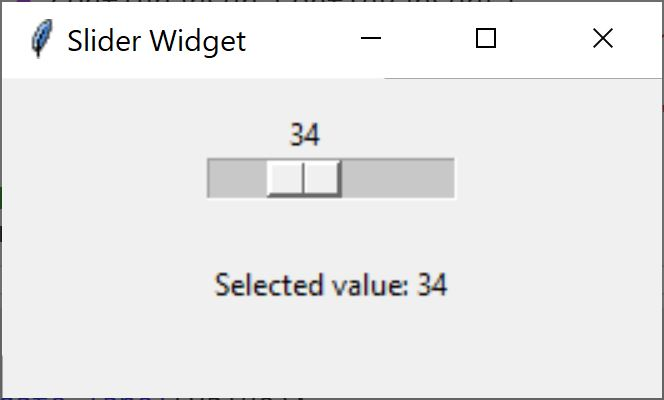
\includegraphics[width=0.4\textwidth]{images/scale_app.JPG}
    \caption{Tkinter Scale App}
    \label{fig:misc-1}
\end{figure}

\newpage
\subsubsection{Tkinter}
\begin{codebox}
\begin{minted}{python}
import tkinter as tk
 
def change_color(event):
    event.widget.configure(bg="red")

root = tk.Tk()
label = tk.Label(root, text="Click me!")
label.bind("<Button-1>", change_color)
label.pack()
 
root.mainloop()
\end{minted}
\end{codebox}
The labels background color will change to red.

\subsubsection{Tkinter - StringVar}
StringVar is a class that provides variable services for Tkinter entry widgets. StringVar is a class in Tkinter used to manipulate string values of Tkinter variables, especially for widgets like Entry and Label, where text can change dynamically.

\newpage
\subsubsection{What is the name of the most general of all Python exceptions?}

BaseException: Exceptions are represented as classes, and they are organized in an inheritance hierarchy. The \texttt{BaseException} class is the root of this hierarchy and serves as the base class for all built-in exceptions in Python.

\subsubsection{Exceptions}
\begin{codebox}
\begin{minted}{python}
def compute(a, b):
    try:
        a / b
    except Exception as exc:
        log(exc)
 
def log(exc):
    logfile = open('logfile.txt')  # Oops, we forgot the 'w' mode.
    print(exc, file=logfile)
    logfile.close()
 
 
compute(0, 0)
\end{minted}
\end{codebox}

\begin{itemize}
\item \textbf{It's an example of implicit exception chaining.} Implicit exception chaining occurs when an exception is caught and a new exception is raised, implicitly attaching the original exception as the cause of the new exception. In this code, the ZeroDivisionError exception is caught in the compute function, and a new exception is raised in the log function. The original exception, ZeroDivisionError, becomes the cause of the new exception.


\item \textbf{This code will raise the ZeroDivisionError exception followed by the FileNotFoundError exception.} In the compute function, the division a / b raises a ZeroDivisionError exception because it attempts to divide by zero. This exception is caught and passed to the log function. However, the log function tries to open the logfile.txt file without the write ('w') mode, leading to a FileNotFoundError exception.

\item The code snippet does \textbf{NOT} demonstrate explicit exception chaining. Explicit exception chaining occurs when one exception is explicitly set as the cause of another exception using the \texttt{raise ... from ...} syntax.
\end{itemize}

\subsubsection{Raising Errors}
In a Python application, you have the following code snippet:

\begin{codebox}
\begin{minted}{python}
try:
    value = int("Hello")
except ValueError as e:
    raise TypeError("Invalid type encountered") from e
\end{minted}
\end{codebox}

\textbf{During the execution, a ValueError is raised in the try block. What happens next?}

A TypeError is raised, and it includes a reference to the original ValueError. Correct as Python's exception chaining mechanism (raise from) attaches the original exception (ValueError) to the new one (TypeError), providing context.

\newpage
\subsubsection{Exceptions}

Implicitly and explicitly chained exceptions refer to how one exception is associated with another in Python:

\begin{itemize}
    \item \textbf{Implicitly Chained Exceptions}:
    \begin{itemize}
        \item When an exception is raised within the handling of another exception, Python automatically sets the \textbf{\texttt{\_\_context\_\_}} attribute of the new exception to the original exception. This creates an implicit chain of exceptions, where the new exception's context is the original exception. This behavior allows you to see the full context in which an exception occurred, helping with debugging and error handling.
    \end{itemize}

    \item \textbf{Explicitly Chained Exceptions}:
    \begin{itemize}
        \item Python also allows you to explicitly chain exceptions using the \textbf{\texttt{raise ... from ...}} syntax. This allows you to raise a new exception while explicitly stating that it was caused by another exception.
        \item This can be useful when you want to raise a higher-level exception that encapsulates the original exception.
    \end{itemize}
\end{itemize}


\begin{itemize}
    \item \textbf{\_\_cause\_\_}: This attribute is for explicitly chained exceptions. It represents the cause of the current exception and is set when one exception is explicitly raised from another using the \texttt{raise ... from ...} syntax.
    
    \item \textbf{\_\_context\_\_}: This attribute is for implicitly chained exceptions. It represents the context in which the current exception occurred. It is automatically set when an exception is raised within the handling of another exception.
    
    \item \textbf{\_\_traceback\_\_}: This attribute is for traceback. It represents the stack trace information associated with the exception. It contains information about the sequence of function calls leading up to the exception.
\end{itemize}

\subsubsection{Explicit exception chaining}
\begin{codebox}
\begin{minted}{python}
class MyCustomException(Exception):
    pass
 
 
def compute(val1, val2):
    try:
        result = val1 / val2
    except ZeroDivisionError as e:
        raise MyCustomException from e
    return result
 
 
compute(1, 0)
\end{minted}
\end{codebox}
In this case, the \texttt{raise MyCustomException from e} statement explicitly raises \texttt{MyCustomException} and links it to the \texttt{ZeroDivisionError (e)} as the cause. This is an example of explicit exception chaining, where the developer deliberately associates the new exception with the original one.

\newpage
\subsubsection{User-defined Exceptions}
In Python, when defining a user-defined exception, it is recommended to derive it from the built-in \texttt{Exception} class or one of its subclasses. The \texttt{Exception} class is the base class for all built-in exceptions in Python.

By deriving a user-defined exception from the \texttt{Exception} class, you inherit the behavior and characteristics of the \texttt{Exception} class. This includes features such as message handling, traceback information, and compatibility with exception handling mechanisms in Python.

\subsubsection{What is the expected output of the following code?}
\begin{codebox}
\begin{minted}{python}
class NewError(Exception):
    def __init__(self, name, color):
        self.data = (name, color)
 
 
try:
    raise NewError('New warning!', 'Red alert!')
except NewError as e:
    # print(e.args) # ('New warning!', 'Red alert!')
    print(' '.join(e.args)) # New warning! Red alert!
\end{minted}
\end{codebox}

The \texttt{args} attribute of the \texttt{NewError} exception is initialized with the tuple \texttt{('New warning!', 'Red alert!')} in the \texttt{\_\_init\_\_} method. In the \texttt{except} block, we print the joined elements of this tuple, resulting in the output "New warning! Red alert!".

\subsubsection{\texttt{json.dumps()}}
The \texttt{json.dumps()} function is used to convert Python objects to JSON-formatted strings. Not all Python objects are JSON serializable. When json.dumps() encounters an object that is not serializable, it raises a \textbf{TypeError} exception.

\begin{codebox}
\begin{minted}{python}
import json

# Example Python dictionary
data = {
    "name": "John",
    "age": 30,
    "city": "New York"
}

# Serialize the dictionary to a JSON formatted string
json_string = json.dumps(data)

# Output the JSON formatted string
print(json_string)
\end{minted}
\end{codebox}

\newpage
\subsubsection{Suppose you have the following \texttt{Vector} class and \texttt{ecnode\_vector()} function. What is the result of the following code?}
\begin{codebox}
\begin{minted}{python}
import json

class Vector:
    def __init__(self, *components):
        print(components)   # Output: (1, 2, 3)
        self.components = components
 
    def __repr__(self):
        return f'Vector{self.components}'
 
    def __str__(self):
        return f'{self.components}'
 
 
def encode_vector(v):
    if isinstance(v, Vector):
        print(v.__dict__)   # Output: {'components': (1, 2, 3)}
        return v.__dict__
    else:
        raise TypeError(
            f'Object of type {v.__class__.__name__} is not JSON serializable'
        )

v1 = Vector(1, 2, 3)
print(json.dumps(v1, default=encode_vector))   
# Output: {"components": [1, 2, 3]}
\end{minted}
\end{codebox}

The \texttt{json.dumps()} function is used to serialize Python objects to a JSON formatted string. It takes a Python object (such as a dictionary, list, tuple, etc.) as input and returns a string representing that object in JSON format. The \texttt{default} parameter is an optional parameter that allows you to specify a function that will be called for objects that are not serializable by default. This function should return a serializable version of the object, or raise a \texttt{TypeError} if it cannot do so.

\newpage
\subsubsection{Coding}

\begin{codebox}
\begin{minted}{python}
class IntegerList(list):
 
    @staticmethod
    def check_type(value):
        if type(value) is not int:
            raise ValueError('The value must be of type int.')
 
    def __setitem__(self, index, value):
        IntegerList.check_type(value)
        list.__setitem__(self, index, value)
 
    def append(self, value):
        IntegerList.check_type(value)
        list.append(self, value)        
 
    def extend(self, iterable):
        for element in iterable:
            IntegerList.check_type(element)
        list.extend(self, iterable)
\end{minted}
\end{codebox}

\textbf{Which of the following operations will run without errors?}

\begin{codebox}
\begin{minted}{python}
integers = IntegerList([1, 2, 3])
integers[1] = 0
\end{minted}
\end{codebox}

\begin{codebox}
\begin{minted}{python}
integers = IntegerList([1, 2, 3])
integers.extend([4, 5])
\end{minted}
\end{codebox}

\newpage
\subsubsection{Asterisks in function definition}
\textbf{What do the asterisks in the function definition mean?}\\
They denote parameters that should be unpacked before use. In Python function definitions, the asterisks (\texttt{*} and \texttt{**}) have special meanings when used in the parameter list. They are used to handle variable-length arguments and to unpack iterables or dictionaries.

\begin{itemize}
    \item \textbf{*args}: When an asterisk is prefixed before a parameter name in a function definition (e.g., *args), it allows the function to accept any number of positional arguments. These arguments are packed into a tuple within the function, allowing you to pass a variable number of arguments to the function.
    \item \textbf{**kwargs}: When two asterisks are prefixed before a parameter name in a function definition (e.g., **kwargs), it allows the function to accept any number of keyword arguments. These arguments are packed into a dictionary within the function, allowing you to pass a variable number of keyword arguments to the function.
\end{itemize}

\subsubsection{Function calls}
\begin{codebox}
\begin{minted}{python}
def process_data(*args, **kwargs):
    if "mode" in kwargs:
        mode = kwargs['mode']
        if mode == 'sum':
            result = sum(args)
        elif mode == 'product':
            result = 1
            for arg in args:
                result *= arg
        else:
            result = None
    else:
        result = None
 
    return result
\end{minted}
\end{codebox}
\textbf{Which of the following function calls will correctly compute the product of the given numbers?}

\texttt{process\_data(2, 4, 6, mode='product')}: This function call correctly passes the numbers 2, 4, 6 as non-keyword arguments and specifies the keyword argument 'mode' with the value 'product'. It will correctly compute the product of the numbers.

\newpage
\subsubsection{Dictionaries}
\begin{codebox}
\begin{minted}{python}
def merge_dicts(*dicts, **kwargs):
    merged_dict = {}
    for dictionary in dicts:
        print(dictionary)
        merged_dict.update(dictionary)
    merged_dict.update(kwargs)
    return merged_dict


dict1 = {"name": "John", "age": 30}
dict2 = {"city": "New York", "country": "USA"}
dict3 = {"occupation": "Engineer"}
 
merge_dicts(dict1, dict2, dict3, skill="Python", experience=5)
\end{minted}
\end{codebox}

\subsubsection{Context manager}
In Python, a context manager is an object that is used to manage resources and define setup and teardown actions that need to be performed around a block of code. It allows you to allocate and release resources precisely when they are needed, such as opening and closing files, acquiring and releasing locks, and connecting to and disconnecting from databases.

\begin{codebox}
\begin{minted}{python}
# Using a context manager to open and close a file
with open('example.txt', 'r') as file:
    data = file.read()
    # Perform operations with the file

# At this point, the file is automatically closed
\end{minted}
\end{codebox}
In this example, the \texttt{open()} function returns a file object, which acts as a context manager. When the \texttt{with} statement is executed, it calls the \texttt{\_\_enter\_\_()} method of the file object to open the file. After the code block executes, the \texttt{\_\_exit\_\_()} method is called to close the file, ensuring that the file is properly closed even if an exception occurs within the block.\\

It is not necessary to explicitly call the close() method when using a context manager since it automatically takes care of closing the file.

\end{document}